% =============================================================================
%  单文件版：由 tools/assemble.py 从 main.tex + sections/*.tex 自动装配，
%  手改请改 sections/ 分片后重新装配，否则下次装配会被覆盖。
% =============================================================================
% =============================================================================
%  中文学术译注本：David Grabovsky
%  《Chern–Simons Theory in a Knotshell》（陈–西蒙斯理论与纽结）
%  原文：2022-09-14，38 页，pdfTeX；一篇以 Witten 1989 年 Jones 多项式论文
%        [Commun. Math. Phys. 121 (1989) 351] 为主线的教学性综述
%
%  结构：本文件为装配入口；正文分片在 sections/，插图在 figures/。
%  编译：xelatex main.tex（两遍）
%  中文字体：默认 fontset=fandol（TeX Live 自带，跨平台）；Windows 可改 fontset=windows
%  译注开关：\showyizhutrue -> \showyizhufalse 关闭橙色译注方框与编号
%             \showkeytrue  -> \showkeyfalse  关闭蓝色「本节重点」方框
% =============================================================================
\documentclass[11pt,a4paper]{article}

\usepackage[UTF8, fontset=fandol, heading=true]{ctex}
\usepackage{amsmath}
\usepackage{amssymb}
\usepackage{mathtools}
\usepackage{bm}
\usepackage[a4paper,left=2.5cm,right=2.5cm,top=2.6cm,bottom=2.6cm]{geometry}
\usepackage{graphicx}
\usepackage{xcolor}
\usepackage[most]{tcolorbox}
\usepackage{enumitem}
\usepackage{booktabs}
\usepackage{array}
\usepackage[font=small,labelfont=bf,labelsep=quad]{caption}
\usepackage[sort,compress]{cite}
\usepackage[colorlinks=true,
            linkcolor=blue!45!black,
            citecolor=blue!45!black,
            urlcolor=blue!45!black]{hyperref}

\linespread{1.12}
\setlength{\emergencystretch}{3em}
% ---------------------------------------------------------------------------
% PDF 元数据与书签
% ---------------------------------------------------------------------------
\hypersetup{
  pdftitle={陈--西蒙斯理论与纽结（Chern--Simons Theory in a Knotshell 中文译注本）},
  pdfauthor={David Grabovsky（原著）；中文译注：DeepSeek Harness},
  pdfsubject={Chern--Simons theory, knot invariants, topological field theory},
  pdfkeywords={Chern--Simons, Wilson loop, framing, Jones polynomial, anyon},
  bookmarksnumbered=true
}
\allowdisplaybreaks[3]
\renewcommand{\figurename}{图}
\renewcommand{\tablename}{表}
\renewcommand{\refname}{参考文献}
\renewcommand{\contentsname}{目录}
\renewcommand{\appendixname}{附录}

% ---------------------------------------------------------------------------
% 常用数学宏
% ---------------------------------------------------------------------------
\newcommand{\Z}{\mathbb{Z}}
\newcommand{\R}{\mathbb{R}}
\newcommand{\C}{\mathbb{C}}
\newcommand{\Tr}{\operatorname{Tr}}
\newcommand{\dd}{\mathrm{d}}
\newcommand{\SCS}{S_{\mathrm{CS}}}
\newcommand{\SECS}{S^{\mathrm{E}}_{\mathrm{CS}}}
\newcommand{\sgn}{\operatorname{sign}}
\newcommand{\eqdef}{\equiv}

% ---------------------------------------------------------------------------
% 译注（yizhu）：橙色方框，全局连续编号，可一键关闭
% ---------------------------------------------------------------------------
\newif\ifshowyizhu
\showyizhutrue
\newcounter{yizhu}
\newsavebox{\yizhubox}

\newenvironment{yizhu}[1][]{%
    \refstepcounter{yizhu}%
    \par\medskip
    \ifshowyizhu
        \begin{tcolorbox}[enhanced, breakable, fontupper=\small,
            colback=orange!4!white, colframe=orange!55!black,
            boxrule=0.5pt, arc=2pt, left=6pt, right=6pt, top=4pt, bottom=4pt,
            title={\small\textbf{译注 \theyizhu\if\relax\detokenize{#1}\relax\else\ ——#1\fi}},
            fonttitle=\bfseries, coltitle=black, colbacktitle=orange!12!white,
            toptitle=1pt, bottomtitle=1pt]
    \else
        \setbox\yizhubox\vbox\bgroup
    \fi
}{%
    \ifshowyizhu
        \end{tcolorbox}%
    \else
        \egroup
    \fi
    \par\smallskip
}

% ---------------------------------------------------------------------------
% 本节重点（keytakeaways）：蓝色方框，可一键关闭
% ---------------------------------------------------------------------------
\newif\ifshowkey
\showkeytrue
\newenvironment{keytakeaways}{%
    \par\medskip
    \ifshowkey
    \begin{tcolorbox}[enhanced,
        colback=blue!3!white, colframe=blue!35!black,
        boxrule=0.5pt, arc=2pt, left=6pt, right=6pt, top=4pt, bottom=4pt,
        title={\small\textbf{本节重点}\quad{\footnotesize（译者所加）}},
        fonttitle=\bfseries, coltitle=black, colbacktitle=blue!10!white,
        toptitle=1pt, bottomtitle=1pt]
    \else
        \setbox\yizhubox\vbox\bgroup
    \fi
}{%
    \ifshowkey
        \end{tcolorbox}%
    \else
        \egroup
    \fi
    \par\medskip
}

% ---------------------------------------------------------------------------
% 题名
% ---------------------------------------------------------------------------
\title{陈--西蒙斯理论与纽结\\[6pt]
       {\large\mdseries Chern--Simons Theory in a Knotshell}}
\author{David Grabovsky\\[2pt]
        {\small 原文：2022 年 9 月 14 日，38 页，pdf\TeX}\\[8pt]
        {\normalsize 中文译注本}\\
        {\small 译注与排版：DeepSeek Harness 智能体集群}}
\date{原文 2022 年 9 月 14 日；中译本 2026 年 10 月}

% =============================================================================
\begin{document}

\maketitle

% >>>>>>>>>>>>>>>> sections/s00-front.tex <<<<<<<<<<<<<<<<
% ==== 题名页、摘要、译者说明、目录 ====
\begin{abstract}
\noindent
在这篇教学性综述中，我们介绍并研究一种被称为陈--西蒙斯理论的三维拓扑场论。我们从 $\mathrm{U}(1))$ 作用量的现象学出发：讨论它的经典运动方程、它的量子化以及它的可观测对象。随后我们转向非阿贝尔理论，分别用路径积分与正则两种形式处理它。我们尤其关注流形与纽结的标架化，以及量子理论的几何结构。
\end{abstract}

% [Tutor Note: 物理图像] 原文摘要只有四句，却是全文骨架：U(1) 现象学 -> 量子化 -> 可观测（Wilson 圈）-> 非阿贝尔 -> 路径积分/正则两条leg -> 标架化。读正文时可把每一节对回这四句。
\begin{yizhu}[物理图像]
原文摘要仅四句，却已给出全文骨架：先做 $\mathrm{U}(1))$ 现象学（\S\ref{sec:2}），再做两种量子化（\S\ref{sec:3} 路径积分、\S\ref{sec:4} 正则），最后落在标架化这个技术核心上。阅读时宜把每一节对回这四句，否则容易在 \S\ref{sec:3.3} 的指标定理细节中丢失主线。
\end{yizhu}

\section*{译者说明}
\addcontentsline{toc}{section}{译者说明}

\begin{enumerate}[leftmargin=1.6em,itemsep=4pt,topsep=4pt]
  \item \textbf{底本。}David Grabovsky，\emph{Chern--Simons Theory in a Knotshell}，2022 年 9 月 14 日，38 页（pdf\TeX{} 排版）。这是一篇以 Witten 1989 年关于量子场论与 Jones 多项式的论文 \cite{witten1989} 为主线的\textbf{教学性综述}，作者写作时并非 Witten 本人；正文中凡出现「Witten 表明/证明了……」处，指的都是被综述的 Witten 工作，而非本文作者。
  \item \textbf{编号。}原文带编号的公式共 74 个（(2.1)--(2.31)、(3.1)--(3.32)、(4.1)--(4.7)、(5.1)--(5.4)）。中译本逐个保留原编号（用 \verb|\tag| 锁定），正文交叉引用一律用 \verb|\eqref|，故中译本公式号与原文逐号对应，便于对照阅读。章节号由 \LaTeX{} 自动生成，亦与原文一致。
  \item \textbf{译注。}橙色方框为译者所加的学术批注，分「易错点」「含糊点」「物理图像」「原文疑误」四类；每条批注在源码中另有一行 \verb|% [Tutor Note: 类型] 摘要| 注释，便于检索。在导言区把 \verb|\showyizhutrue| 改为 \verb|\showyizhufalse| 可一键关闭全部译注；蓝色「本节重点」方框由 \verb|\showkeytrue| 控制。两开关全关后，译本即为纯译文。
  \item \textbf{插图。}原文共 5 张位图插图（p.5、p.10、p.23、p.24、p.31），均从原 PDF 无损提取（非屏幕截图），存于 \verb|figures/|，按原位置插入，图号与原文一致。
  \item \textbf{编译。}\verb|xelatex main.tex| 连跑两遍。中文由 \verb|ctex| 宏包处理，故\textbf{必须用 Xe\LaTeX}；如无 Fandol 字体，可把导言区的 \verb|fontset=fandol| 改为 \verb|fontset=windows|（Windows 自带宋体/黑体）。
  \item \textbf{存疑。}原文中经核对属笔误或论证不严处，正文一律照录，另加「原文疑误」译注说明，并在 \verb|README.md| 的疑点清单中登记；中译本不作静默修正。
\end{enumerate}

\newpage
\tableofcontents
\newpage
% >>>>>>>>>>>>>>>> end sections/s00-front.tex <<<<<<<<<<<<<<<<

% >>>>>>>>>>>>>>>> sections/s01-intro.tex <<<<<<<<<<<<<<<<
% ==== 原文 p.2 ====
\section{引言与动机}\label{sec:1}

% [Tutor Note: 本节重点] 物理图像/数学工具/主要结论
\begin{keytakeaways}
\begin{itemize}[leftmargin=1.4em,itemsep=2pt,topsep=2pt]
  \item \textbf{物理图像：}陈--西蒙斯理论是三维拓扑场论的典型样本：它没有局部自由度，全部物理内容都藏在全局拓扑里——Wilson 圈沿纽结取值，其期望值给出纽结不变量。
  \item \textbf{数学工具：}微分形式的陈--西蒙斯 $3$-形式 $A\wedge dA$（非阿贝尔情形加 $\frac{2}{3}A^3$）、主丛上的联络与和乐、$4$ 维示性类（Chern--Weil 理论）、路径积分与正则量子化。
  \item \textbf{主要结论：}Witten 表明，Wilson 圈的路径积分期望值是 Jones 多项式的推广；能级 $k$ 必须取整数；该理论在二维共形场论、凝聚态、三维量子引力等处反复出现。本综述将把该理论「发展两遍」：先阿贝尔（\S\ref{sec:2}，沿 Dunne \cite{dunne}），再一般情形（\S\ref{sec:3}--\S\ref{sec:4}，沿 Witten \cite{witten1989}）。
\end{itemize}
\end{keytakeaways}

\paragraph{引言}
陈--西蒙斯理论是拓扑学的简洁、优美与怪异的一次演练。它是拓扑场论的典型样本：这是一种量子场论，其物理可观测对象是理论所在时空的拓扑不变量。具体说来，Witten 在 1980 年代末表明：陈--西蒙斯（CS）理论中被称为\textbf{威尔逊圈}的非局域可观测对象——在三维时空里由纽结表示——会计算这些纽结的某些不变量，而它们正是著名的 Jones 多项式的推广 \cite{witten1989}。作为这项工作的一部分，Witten 说明了如何用路径积分给这类不变量以物理解释；这项工作为他赢得了菲尔兹奖。他还量子化并求解了该理论，给出了其希尔伯特空间结构的描述。他的工作揭示了数学与物理众多领域之间的深刻联系，并激起了一连串研究活动，极大地丰富并联结了这两个领域。

% [Tutor Note: 含糊点] 「Witten 表明 Wilson 圈计算 Jones 多项式」的具体含义：G=SU(2)、M=S^3 时 Z(S^3,L) 就是 Jones 多项式；且 Witten 的路径积分论证与 Reshetikhin–Turaev 的严格代数构造是两条独立路线，前者物理、后者严格。
\begin{yizhu}[含糊点]
「Wilson 圈计算纽结不变量」一句在此只是断言，其确切含义要到 \S\ref{sec:3.1} 末才给出：当 $G=\mathrm{SU}(2))$、$M=S^3$ 时，带链环 $L$ 的配分函数 $Z(S^3,L)$ 恰为 $L$ 的 Jones 多项式。另需知道，Witten 用的是路径积分论证（物理上直观，但需正规化），而 Reshetikhin--Turaev 后来用量子群与辫群表示给出了同一不变量的严格组合构造；两条路线给出的不变量一致，这是 CS 理论最重要的可检验性之一。
\end{yizhu}

\paragraph{动机}
CS 理论出现在二维共形场论、三维量子引力、四维规范场论、凝聚态物理、几何、拓扑等领域之中。这里的寓意是：本综述对每个人都该有点用处。

\begin{itemize}[leftmargin=1.4em,itemsep=4pt,topsep=2pt]
  \item 在\textbf{杨--米尔斯理论}中，用于描述孤子、瞬子、磁单极子与反常的 $\theta$ 项伴随着一个拓扑荷。这个荷的量子化与 CS 理论的量子化类似；四维费米子的许多性质，可以看作低一维的 CS 物理的回声。
  \item 在\textbf{二维共形场论}（CFT）中，与 CS 理论的一些出人意料的联系以微妙的方式显现出来。费米子的行为、韦斯--朱米诺--维滕模型的物理、仿射 Kac--Moody 代数的表示，以及有理共形场论，都可以透过 CS 理论的这面三维透镜得到解释。
  \item 在\textbf{凝聚态理论}中，拓扑绝缘体与分数量子霍尔效应都由含 CS 项的低能有效作用量支配。把物质耦合到 CS 项上，会产生大量新奇的拓扑现象与拓扑相。此外，朗道能级的物理在阿贝尔 CS 理论的形式解中也有应用。
  \item 在\textbf{微分几何与拓扑学}中，人们用示性类、Chern--Weil 理论等工具研究各种主丛及其（主）联络的曲率。CS 形式、它的规范论性质以及由它产生的不变量，构成了这一学科的基础，反过来也指导了对 CS 理论本身的研究。
  \item 在\textbf{纽结理论}中，Witten 的工作直接给出了许多拓扑不变量的物理的、内蕴三维的实现与推广，其中包括 Reidemeister 挠率、雷--辛格挠率、Jones 多项式以及 Khovanov 同调。
  \item 在\textbf{量子引力}中，Witten 表明三维引力可以改写为一个规范群非紧的 CS 理论，并可以精确求解。随着全息对偶的出现，这一进展把 CS 理论推到了现代低维量子引力研究的最前沿。
\end{itemize}

% [Tutor Note: 原文疑误] Khovanov 同调（1999 年才由 Khovanov 定义）的物理实现并非 Witten 1989 年工作的直接产物，而是后来的 fivebrane/拓扑弦构造（Witten 2011；Gukov–Schwarz–Vafa 2005）；原文把它并列进「直接给出」的清单，史实上不准确。
\begin{yizhu}[原文疑误]
把 Khovanov 同调列入「Witten 的工作直接给出的实现」在史实上不准确。Jones 多项式才有 1989 年 CS 框架下的直接路径积分实现；Khovanov 同调（1999）的物理解释一般归功于后来的 fivebrane 与拓扑弦构造（Witten 2011, \emph{Fivebranes and Knots}；Gukov--Schwarz--Vafa 2005）。原文此句宜读作「该框架在后来的发展中覆盖了这些不变量」。中译本照录原文，不作改写。
\end{yizhu}

\paragraph{结构安排}
在本综述中，我们将描述 Witten 工作的若干侧面。我们会把 CS 理论\textbf{发展两遍}：先在阿贝尔情形（\S\ref{sec:2}）中沿 Dunne \cite{dunne} 进行，再在一般情形（\S\ref{sec:3}--\S\ref{sec:4}）中沿 Witten 的里程碑式论文 \cite{witten1989} 进行。阿贝尔情形将作为热身：在那里我们会看到 CS 理论的一些关键特征，例如任意子、威尔逊圈、环绕数、它的规范行为，以及它量子化中的一些微妙之处。这将构成我们对 CS 物理的直观理解的核心；综述其余部分的形式化发展既依赖于这些想法，也将把它们充实起来。在 \S\ref{sec:3} 中，我们会强调路径积分以及纽结的标架化所起的作用。对这个初看像是迂腐麻烦的问题作细致考察，将使我们能显式地在弱耦合下计算 CS 路径积分。随后在 \S\ref{sec:4} 中，我们会描述该理论的正则量子化，采取基于各种模空间上线丛的全纯路线。在那里我们将容许自己稍微含糊一些，以求把要点讲清。我们将基本回避纽结多项式的讨论，但会在 \S\ref{sec:5} 中简要提及它们，并连同另外几件杂事一起为讨论收尾。

% [Tutor Note: 易错点] 全文号差约定在 \\ 处由 Lorentz 号差切换到欧氏号差；这一切换使 (2.1) 的 S_CS 变为纯虚、从而保证 e^{-S^E} 的相位性，是 (2.12) 能级量子化论证的前提。读后半篇时若仍按 §2 号差算，会得到符号相反的 F^2 项。
\begin{yizhu}[易错点]
全文的号差约定在 \S\ref{sec:3} 处悄悄切换：\S\ref{sec:2} 用 Lorentz 号差（mostly minus，即 $(+,-,-)$），从 \S\ref{sec:3} 起改用欧氏号差并保持到文末。这一切换并非形式上的小事：正因 CS 作用量在欧氏号差下变成纯虚的 $\SECS=-i\SCS$，$e^{-\SECS}=e^{i\SCS}$ 才是纯相位，\S\ref{sec:2.2} 中「路径积分在 $k\in\Z$ 时规范不变」的论证才成立。若在后半篇误用 Lorentz 号差，$F^2$ 项整体会变号。
\end{yizhu}

\paragraph{约定}
我们在 \S\ref{sec:2} 中先采用 Lorentz 号差，并使用 mostly minus 约定。然而从 \S\ref{sec:3} 开始，我们将切换到欧氏号差，并在综述余下部分一直保持。时空指标用希腊字母 $\mu,\nu,\rho\in\{0,1,2\}$，空间指标用中段拉丁字母 $i,j,k\in\{1,2\}$。全文采用爱因斯坦求和约定，另有说明者除外。需要提醒的是：字母 $g$ 会分别指三维流形上的度规、规范群的一个元素，或黎曼面的亏格，其含义须由上下文判断。

% [Tutor Note: 原文疑误] 原文此段 "Starting with \\, however, however, we will switch..." 重复了一个 however，属排印重复；译文按单次 however 处理，特此说明。
\begin{yizhu}[原文疑误]
原文此处作「Starting with \S3, however, however, we will switch to Euclidean signature」，连写两个 however，属排印重复（原文 p.3）。译文按单次处理；若对照英文原文阅读，此处无需再找第二个转折。
\end{yizhu}

% [Tutor Note: 易错点] 字母 g 的三重身份是全文最常见的记号陷阱：度规 g（出现在 2.29、3.25 的 |g| 与 {\rm Tr}(ω dω+…) 的构造中）、群元 g(x)（(3.1)、(3.4)、(3.5)）、亏格 g（4.3、4.7 与 d(2g−2)）。
\begin{yizhu}[易错点]
字母 $g$ 的三重身份是全文最常见的记号陷阱，务必在每一步先确认它指的是哪一个：
（1）\textbf{度规}——出现在能动张量 \eqref{eq:2.29} 的 $\sqrt{|g|}$、引力 CS 项 \eqref{eq:3.25} 所依赖的度规，以及流形标架化问题中；
（2）\textbf{规范群元素}——\eqref{eq:3.1} 的 $A_\mu\to g^{-1}A_\mu g+g^{-1}\partial_\mu g$ 与绕数 \eqref{eq:3.5} 中的 $g(x)$；
（3）\textbf{亏格}——\S\ref{sec:4} 中黎曼面 $\Sigma$ 的亏格，以及模空间维数 $d(2g-2)$。
把 (3) 与 (1)(2) 混淆，是读 \S\ref{sec:4} 时最常见的错误来源。
\end{yizhu}
% >>>>>>>>>>>>>>>> end sections/s01-intro.tex <<<<<<<<<<<<<<<<

% >>>>>>>>>>>>>>>> sections/s02a-abelian.tex <<<<<<<<<<<<<<<<
% =============================================================================
%  s02a-abelian.tex —— §2 阿贝尔陈--西蒙斯理论（引言、2.1、2.2）
%  覆盖原文 p.3（"The theory of Chern and Simons."）— p.9（"CS theory is really
%  good at doing this."）
%  编号公式 (2.1)--(2.19)，图 1（fig:universe），脚注 1、2
% =============================================================================

% ==== 原文 p.3 ====
\section{阿贝尔陈--西蒙斯理论}\label{sec:2}

% [Tutor Note: 本节重点] 物理图像 / 数学工具 / 主要结论 三条
\begin{keytakeaways}
\begin{itemize}[leftmargin=1.4em,itemsep=2pt,topsep=2pt]
  \item \textbf{物理图像：} 3 维 $\mathrm{U}(1)$ 陈--西蒙斯项对 $A$ 是一阶的，没有传播自由度；电荷自带磁通 $\rho=\frac{k}{2\pi}B$，绕电荷一周即得阿哈罗诺夫–玻姆相位，双次交换给出任意子相位 $e^{2\pi i/k}$。
  \item \textbf{数学工具：} 运动方程 $F=0$ 即平坦联络；库仑规范下的解 \eqref{eq:2.7} 是纯规范；高斯环绕积分 $\Phi[\gamma_1,\gamma_2]$ 把威尔逊圈期望值写成环绕数的指数，见 \eqref{eq:2.19}。
  \item \textbf{主要结论：} 大规范变换使 $S_{\mathrm{CS}}\to S_{\mathrm{CS}}+2\pi k$，量子化要求 $k\in\Z$；$\langle W_1W_2\rangle=\exp\!\left(\frac{2\pi i}{k}\Phi\right)$ 表明 CS 理论在计算纽结的环绕数。
\end{itemize}
\end{keytakeaways}

\paragraph{陈与西蒙斯的理论} % 原文标题：The theory of Chern and Simons.
我们不必一头扎进抽象形式，先看一个简单而有教益的例子。设 3 维闵可夫斯基空间 $M=\R^{2,1}$ 代表宇宙。阿贝尔陈--西蒙斯作用量由 $\mathrm{U}(1)$ 规范场 $A_\mu(x)$ 构造，它类似电动力学中的光子场：
\begin{equation}\tag{2.1}\label{eq:2.1}
  S_{\mathrm{CS}}[A] \equiv \frac{k}{4\pi}\int_M \dd^3x\,\varepsilon^{\mu\nu\rho}A_\mu\partial_\nu A_\rho .
\end{equation}

% ==== 原文 p.4 ====
其中 $\varepsilon^{\mu\nu\rho}$ 是全反对称符号，$k\in\R$ 称为陈--西蒙斯能级（level），因子 $\frac{1}{4\pi}$ 纯属约定。这个作用量有点古怪：它只在 3 维才有意义，而且对 $A$ 的导数是一阶的。为了对其行为建立直觉，我们来考察它所定义的理论的经典后果与量子后果。

我们跟随 Dunne 的综述 \cite{dunne}，偶尔借重 Tong 的洞见 \cite{tong_gauge,tong_qhe}。

\subsection{经典理论}\label{sec:2.1}

\paragraph{运动方程} % 原文标题：The equations of motion.
由作用量 \eqref{eq:2.1} 得出的运动方程是
\begin{equation}\tag{2.2}\label{eq:2.2}
  \delta S_{\mathrm{CS}} = 0 \;\Longrightarrow\; \frac{k}{4\pi}\varepsilon^{\mu\nu\rho}F_{\nu\rho} = 0
  \;\Longrightarrow\; F = 0, \qquad F_{\mu\nu} = \partial_\mu A_\nu - \partial_\nu A_\mu .
\end{equation}
这显得相当乏味：没有传播的局部自由度，常数 $k$ 也不影响经典物理。加入物质可以补救。例如，狄拉克费米子 $\psi$ 通过一个流与 CS 项耦合：
\begin{equation}\tag{2.3}\label{eq:2.3}
  \mathcal{L} = \frac{k}{4\pi}\varepsilon^{\mu\nu\rho}A_\mu\partial_\nu A_\rho
  + \bar{\psi}\left(i\not\partial - m\right)\psi
  - eA_\mu\bar{\psi}\gamma^\mu\psi
  = \mathcal{L}_{\mathrm{CS}} + \mathcal{L}_\psi + A_\mu J^\mu .
\end{equation}
用物质流 $J$ 表示，\eqref{eq:2.3} 给出的 $A$ 的运动方程为
\begin{equation}\tag{2.4}\label{eq:2.4}
  \frac{k}{4\pi}\varepsilon^{\mu\nu\rho}F_{\nu\rho}
  = \frac{k}{2\pi}\varepsilon^{\mu\nu\rho}\partial_\nu A_\rho = J^\mu .
\end{equation}

% [Tutor Note: 易错点] (2.4) 的 4π→2π 来自 F_{νρ} 两项相等，因子 2 不可漏
\begin{yizhu}[易错点]
把 \eqref{eq:2.2} 的 $F_{\nu\rho}=\partial_\nu A_\rho-\partial_\rho A_\nu$ 代入：$\varepsilon^{\mu\nu\rho}F_{\nu\rho}=2\varepsilon^{\mu\nu\rho}\partial_\nu A_\rho$，两项因 $\varepsilon$ 全反对称而相等。这就是 \eqref{eq:2.4} 中 $\frac{k}{4\pi}\to\frac{k}{2\pi}$ 的来源。漏掉因子 2，就与 \eqref{eq:2.2} 的系数 $\frac{k}{4\pi}$ 自相矛盾——那里右端恰为 $F=0$，把这一层掩盖了。
\end{yizhu}

\paragraph{插一段几何} % 原文标题：Geometrical aside.
后文会讲到，$A$ 其实是 $M$ 上某个主 $\mathrm{U}(1)$ 丛上的联络，拉格朗日量是陈--西蒙斯 3 形式 $A\wedge\dd A$ 的倍数。场强 $F=\dd A$ 就是该联络的曲率，于是运动方程 $F=0$ 描写平坦联络。物质流 $J$ 的存在把运动方程改为 $\frac{k}{4\pi}\star F=J$（$\star$ 是霍奇星算子），物质于是在规范丛中引入曲率。奇妙的是，这个曲率可以由时空的一个拓扑不变量测量，而该不变量由 CS 形式构造。这一事实是陈--韦伊理论的起点；在数学家看来，那才是研究 CS 作用量的正路 \cite{chern1974}。

\paragraph{电场与磁场} % 原文标题：Electric and magnetic fields.
场强张量 $F_{\mu\nu}$ 由电场 $\mathbf{E}$ 与磁场 $B$ 组成，二者的定义与麦克斯韦理论完全相同：
\begin{equation}\tag{2.5}\label{eq:2.5}
  E_i \equiv -\partial_i A_0 - \partial_0 A_i, \qquad B \equiv \varepsilon^{ij}\partial_i A_j .
\end{equation}
把物质流 $J^\mu\equiv(\rho,\mathbf{J})$ 写成电荷密度与电流密度，直接验证即知 CS 运动方程的分量形式为
\begin{equation}\tag{2.6}\label{eq:2.6}
  \rho = \frac{k}{2\pi}B, \qquad J^i = \frac{k}{2\pi}\varepsilon^{ij}E_j .
\end{equation}

% [Tutor Note: 易错点] (2.6) 依赖 ε^{0ij}=ε^{ij} 与 ε^{ij0}=+ε^{ij} 的指标约定
\begin{yizhu}[易错点]
由 \eqref{eq:2.4} 的 $\mu=0$ 分量得 $J^0=\frac{k}{2\pi}\varepsilon^{0ij}\partial_iA_j$；要得到 \eqref{eq:2.6} 的 $\rho=\frac{k}{2\pi}B$，必须取 $\varepsilon^{0ij}=+\varepsilon^{ij}$（即 $\varepsilon^{012}=+1$、二维 $\varepsilon^{12}=+1$）。$\mu=i$ 分量还需要 $\varepsilon^{ij0}=+\varepsilon^{ij}$ 与 $\varepsilon^{i0j}=-\varepsilon^{ij}$。换一种升降约定，$J^i$ 里的 $\varepsilon^{ij}E_j$ 会整体变号。
\end{yizhu}

% [Tutor Note: 原文疑误] (2.5) 的 E_i 与 (2.6) 的 ε^{ij}E_j 仅在 A_0=0 时自洽
\begin{yizhu}[原文疑误]
取纯电场位形 $A_\mu=(A_0(x),0)$：由 \eqref{eq:2.4} 得 $J^1=\frac{k}{2\pi}\varepsilon^{120}\partial_2A_0=+\frac{k}{2\pi}\partial_2A_0$；而 \eqref{eq:2.6} 配 \eqref{eq:2.5} 给出 $J^1=\frac{k}{2\pi}\varepsilon^{12}(-\partial_2A_0)=-\frac{k}{2\pi}\partial_2A_0$，两者差一个符号（$A_0\neq0$ 时一般差 $2\partial_jA_0$ 项）。原文照录。全节随后都取库仑规范 $A_0=0$，故不影响 \eqref{eq:2.7} 以下的结论。
\end{yizhu}

% ==== 原文 p.5 ====
显然 $B$ 由电荷产生，而 $\mathbf{E}$ 是电流的后果：这与电磁学的情形正好相反。图~\ref{fig:universe} 左画出了这一物理图像：运动的电荷在平面内产生 $\mathbf{E}$ 场，它们的 $B$ 场则指向一个虚构的“$z$”方向。（这幅图在霍尔物理中其实与实验相符。）每条磁通线都附着在一个源电荷上，并穿透空间流形。

% [Tutor Note: 物理图像] 电荷自带磁通，所以绕行相位只依赖环绕数
\begin{yizhu}[物理图像]
\eqref{eq:2.6} 的第一式说明电荷与磁通绑定：一个电荷必拖着一束 $B$ 通量。于是“绕过电荷”等价于“绕过一束磁通”，阿哈罗诺夫–玻姆相位只依赖回路绕这束通量的圈数。任意子相位之所以是拓扑量，根源就在这里。
\end{yizhu}

\begin{figure}[htbp]
  \centering
  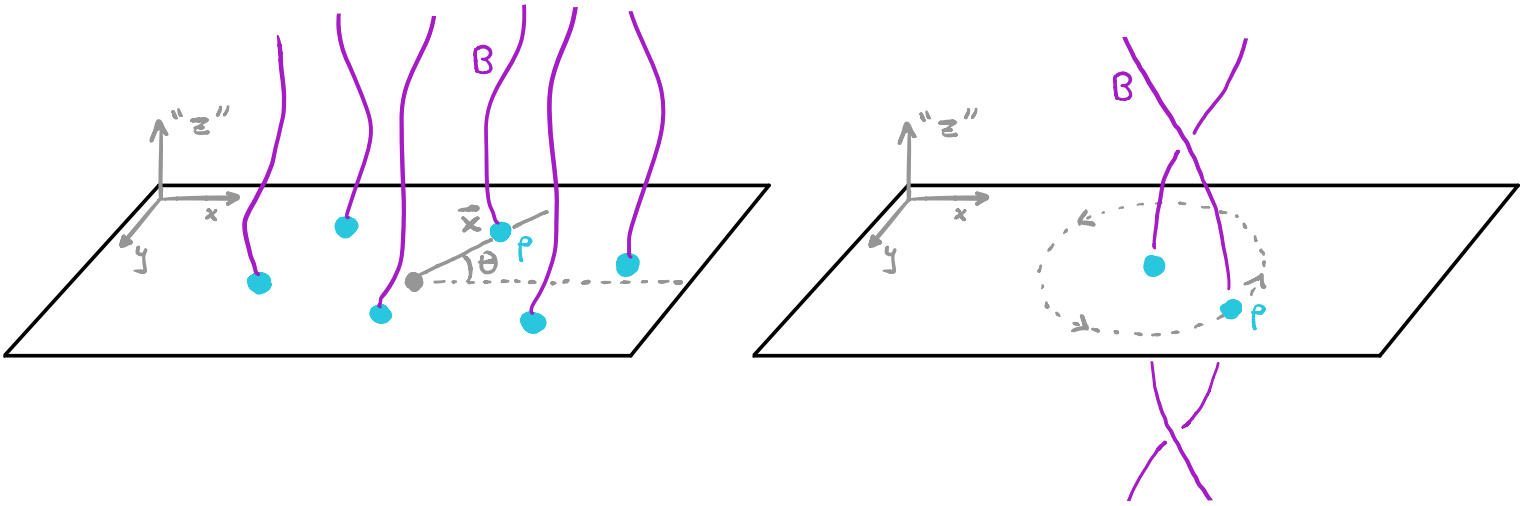
\includegraphics[width=0.95\textwidth]{figures/fig1_cs_universe_anyon.png}
  \caption{左：陈--西蒙斯宇宙。右：一个任意子！（原文 Figure 1，原文 p.5）}
  \label{fig:universe}
\end{figure}

\paragraph{单个检验电荷} % 原文标题：A single test charge.
为了更细致地理解其中的物理，我们来解 CS 方程 \eqref{eq:2.6}，取源为 $\rho=\delta^{(2)}(\mathbf{x}-\mathbf{x}_a(t))$ 与 $\mathbf{J}=\mathbf{0}$。取库仑规范，即 $A_0=0=\partial_iA^i=\nabla\cdot\mathbf{A}$。把这两个源代入 \eqref{eq:2.6}，按 \eqref{eq:2.5} 用 $A_\mu=(0,A_i)$ 写出 $\mathbf{E}$ 与 $B$ 场，再用标准的格林函数技术（具体说，用恒等式 $\nabla^2\log|\mathbf{x}|=2\pi\delta^{(2)}(\mathbf{x})$），即得 \eqref{eq:2.6} 的解：
\begin{equation}\tag{2.7}\label{eq:2.7}
  A_i(\mathbf{x},t) = \frac{1}{k}\varepsilon_{ij}\frac{x^j - x_a^j(t)}{|\mathbf{x}-\mathbf{x}_a|^2}
  = -\frac{1}{k}\partial_i\theta(\mathbf{x}-\mathbf{x}_a(t)),
  \qquad \theta(\mathbf{x}) \equiv \tan^{-1}\!\left(\frac{y}{x}\right) = \arg(\mathbf{x}) .
\end{equation}

% [Tutor Note: 易错点] (2.7) 用下标 ε_{ij}、(2.6) 用上标 ε^{ij}，联立时符号最易出错
\begin{yizhu}[易错点]
取二维 $\varepsilon_{12}=+1$，由 \eqref{eq:2.7} 绕源一周得 $\oint A_i\dd x^i=-2\pi/k$，故 $B=\varepsilon^{ij}\partial_iA_j=-\frac{2\pi}{k}\delta^{(2)}(\mathbf{x}-\mathbf{x}_a)$，代回 \eqref{eq:2.6} 得 $\rho=-\delta^{(2)}$，与正文所取 $+\delta^{(2)}$ 相差一个整体符号。原文照录；凡核对 (2.6) 与 (2.7) 的符号，先固定 $\varepsilon_{12}$ 与 $\varepsilon^{12}$ 的取值，再以 \eqref{eq:2.9} 的 $e^{+i\theta/k}$ 与 \eqref{eq:2.19} 的 $+2\pi i/k$ 为基准。
\end{yizhu}

% [Tutor Note: 含糊点] “standard Green's function techniques” 跳过二维库仑格林函数的构造
\begin{yizhu}[含糊点]
作者省略的求解链条是：由 \eqref{eq:2.6} 与点源得 $\varepsilon^{ij}\partial_iA_j=\frac{2\pi}{k}\delta^{(2)}(\mathbf{x}-\mathbf{x}_a)$，而 $\partial_j\log|\mathbf{x}|=x^j/|\mathbf{x}|^2$，故取 $A_i=\frac{1}{k}\varepsilon_{ij}\partial_j\log|\mathbf{x}-\mathbf{x}_a|$ 即得 \eqref{eq:2.7}。所用定理是二维库仑格林函数恒等式 $\nabla^2\log|\mathbf{x}|=2\pi\delta^{(2)}(\mathbf{x})$（三维对照式 $\nabla^2\frac{1}{|\mathbf{x}|}=-4\pi\delta^{(3)}(\mathbf{x})$），见原文 [10]。
\end{yizhu}

注意 $A_i$ 是全导数：它是纯规范位形。取规范参数 $\omega(\mathbf{x})\equiv\left(\frac{1}{k}\right)\theta(\mathbf{x}-\mathbf{x}_a(t))$，相应的规范变换加上 $\omega$ 的全导数，就把它化为零。于是 $A(x)\equiv0$，$\mathbf{E}\equiv\mathbf{0}$、$B=0$ 都成了平凡结论。但同一个规范变换也作用在物质场 $\psi$ 上——它正是源电荷的载体——给它一个非平凡的阿哈罗诺夫–玻姆相位，该相位取决于角位置 $\theta$ 与 $k$：
\begin{equation}\tag{2.8}\label{eq:2.8}
  \omega = \frac{1}{k}\theta \;\Longrightarrow\;
  \begin{cases}
    A_i(x) \longrightarrow A'(x) = A_i(x) + \partial_i\omega(x) = 0,\\[2pt]
    \psi(x) \longrightarrow \psi'(x) = e^{i\omega(x)}\psi(x) = e^{i\theta/k}\psi(x).
  \end{cases}
\end{equation}

% [Tutor Note: 原文疑误] (2.8) 首行 A'(x) 漏掉下标 i
\begin{yizhu}[原文疑误]
\eqref{eq:2.8} 首行左端是 $A_i(x)$，右端却写 $A'(x)$ 无下标，同一行的 $A_i(x)+\partial_i\omega(x)$ 又带下标 $i$。按下标一致性应读作 $A'_i(x)$。原文字面照录，译文不改。
\end{yizhu}

% [Tutor Note: 原文疑误] p.5 “Aharanov-Bohm” 应为 Aharonov–Bohm
\begin{yizhu}[原文疑误]
原文 p.5 此处拼作 “Aharanov-Bohm”，标准拼写是 Aharonov–Bohm（阿哈罗诺夫–玻姆）。属拼写笔误，译文按规范术语处理，原文拼写照录于此。
\end{yizhu}

\paragraph{双次交换与任意子} % 原文标题：Double exchange and anyons.
现在考虑两个电荷，如图~\ref{fig:universe} 右。一个保持静止，另一个绕它运动。我们把这一过程看作双次交换：运动的电荷与静止的电荷交换位置两次，每转 $\pi$ 一次。

% ==== 原文 p.6 ====
由 \eqref{eq:2.8}，运动粒子得到的相位为
\begin{equation}\tag{2.9}\label{eq:2.9}
  \Delta\theta = 2\pi \;\Longrightarrow\;
  \psi(x) \longrightarrow \exp\!\left(\frac{2\pi i}{k}\right)\psi(x)
  = \exp\!\left(i\oint_{\theta=0}^{\theta=2\pi}\dd x^i A_i\right)\psi(x) \neq \psi(x) .
\end{equation}

% [Tutor Note: 含糊点] (2.9) 末端的 ψ(x)≠ψ(x) 左右同一记号
\begin{yizhu}[含糊点]
\eqref{eq:2.9} 末端写作 $\psi(x)\neq\psi(x)$，两边记号相同，因为原文对变换后的场仍写 $\psi(x)$（\eqref{eq:2.8} 里写的是 $\psi'(x)$）。读时应把右端理解为 $\psi'(x)$：绕行一周后波函数只差一个相位，不是同一个态。相位 $\exp(2\pi i/k)$ 正是 \eqref{eq:2.8} 第二式取 $\theta=2\pi$ 的结果。
\end{yizhu}

若这些粒子是玻色子或费米子，$\psi$ 在双次交换后会回到自身。但 \eqref{eq:2.9} 表明，调节 $k$ 就能赋予 $\psi$ 取值于 $\mathrm{U}(1)$ 的任意统计。所以这些粒子是任意子，因为它们可以有任意统计。（量 $e^{2\pi i/k}$ 与 $A$ 的闭合回路积分的指数式，会在本综述中反复出现。）

\paragraph{几点评论} % 原文标题：Comments.
任意子得到的相位只依赖 $k$ 与所走路径的拓扑。在我们的例子里，它绕静止电荷在 $\R^2$ 上扎出的一个穿孔点转了一圈（该点处电荷为无穷大）。可见 CS 理论自带一个场论探针——任意子相位——它能探测 $\R^2\backslash\{\mathbf{0}\}\simeq S^1\times\R$ 中非平凡回路的绕数。同一想法的另一个反映，是图~\ref{fig:universe} 中磁通线的缠绕。下面会看到，把这些磁通线看成在无穷远处闭合的回路——也就是纽结——很有用。这一视角不仅给出高斯定律的一幅图像，还揭示出 CS 理论实际上在计算这些 $B$ 场纽结的环绕数。要点在于：CS 理论没有局部自由度，却强烈影响相距很远的粒子，并且知道红外物理 \cite{tong_gauge}。

\subsection{路径积分量子化}\label{sec:2.2}

\paragraph{规范不变吗？} % 原文标题：Gauge invariance?
讨论任意子时，我们已经看到 CS 理论在规范变换下的性质。现在转向一个更简单也更基本的问题：我们要证明纯 CS 作用量 \eqref{eq:2.1} 不是规范不变的。这个项目一开始就极不顺利：在形如 $A_\mu\to A'_\mu=A_\mu+\partial_\mu\omega$ 的规范变换下，计算表明作用量改变一个全导数：
\begin{equation}\tag{2.10}\label{eq:2.10}
  S_{\mathrm{CS}} \longrightarrow S'_{\mathrm{CS}} = S_{\mathrm{CS}}
  + \frac{k}{4\pi}\int_M \dd^3x\,\varepsilon^{\mu\nu\rho}\partial_\mu(\omega\,\partial_\nu A_\rho) .
\end{equation}
若 $\omega$ 在无穷远处为零，边界项为零，$S_{\mathrm{CS}}$ 就规范不变。尴尬的是，即使 $\omega$ 在无穷远处不为零，只要没有磁单极子，由高斯定律，阿贝尔 CS 作用量仍然规范不变。\footnote{正如我们将看到的，非阿贝尔理论并非如此，它更脆弱：所有“大”规范变换（large gauge transformation）都使作用量发生非平凡变换，无需向理论中添加磁单极子。由此得到的变换 $S_{\mathrm{CS}}\to S_{\mathrm{CS}}+2\pi k$，与带磁单极子的阿贝尔理论相同。} 因此我们来描写磁通破坏规范不变性的最简单情形。最终，一个精心挑选的规范变换会让作用量按 $S_{\mathrm{CS}}\to S_{\mathrm{CS}}+2\pi k$ 变换。下面会看到，这意味着在量子理论中 $k$ 必须是整数。

% [Tutor Note: 含糊点] “由高斯定律仍规范不变”一句跳过了边界项为零的论证
\begin{yizhu}[含糊点]
这句“即使 $\omega$ 在无穷远处不为零……仍然规范不变”没有给证明。由 \eqref{eq:2.10}，$\delta S_{\mathrm{CS}}=\frac{k}{4\pi}\int_M\dd^3x\,\partial_\mu(\omega\varepsilon^{\mu\nu\rho}\partial_\nu A_\rho)$ 是全导数的积分，化为空间无穷远 $S^2$ 上的通量 $\oint_{S^2}\omega\,B\,\dd S$。没有磁单极子时 $\oint_{S^2}B\,\dd S=0$（高斯定律，斯托克斯定理的直接推论），故为零。下一段正是靠“引入磁通”打破这一零。见原文 [10]。
\end{yizhu}

% ==== 原文 p.7 ====
\paragraph{欧氏空间的杂技} % 原文标题：Euclidean acrobatics.
要打破 $S_{\mathrm{CS}}$ 的规范不变性，最省事的办法是把空间流形紧致化为 $S^2$，再经威克转动 $t\to\tau=it$ 转到欧氏号差，时间轴 $\R$ 于是变成热圆周 $S^1$。关键在于，CS 作用量对时间导数是一阶的，它变换为 $S_{\mathrm{CS}}\to S^{\mathrm{E}}_{\mathrm{CS}}=-iS_{\mathrm{CS}}$。接着选规范变换 $\omega(\tau,\mathbf{x})=\frac{2\pi\tau}{\beta}$，它绕热圆周转一整圈，不能连续形变为恒等映射。最后引入磁通，即 $B=F_{12}$ 在 $S^2$ 上的非零积分。为此设想 $S^2\subset\R^3$ 包围一个安放在原点的磁单极子，再测穿过其表面的通量。念及狄拉克，我们回想起 $\mathrm{U}(1)$ 的紧致性使这类通量量子化：
\begin{equation}\tag{2.11}\label{eq:2.11}
  \int_{S^2} F_{12} = 2\pi n, \qquad n\in\Z .
\end{equation}
至此，全部配料齐备：考虑 $M=S^2\times S^1$ 上的规范变换 \eqref{eq:2.10}，代入上面给出的 $\omega$。分部积分表明，边界项正比于上面的通量积分；取 $n=1$，得 $\delta S_{\mathrm{CS}}=2\pi k$。

% [Tutor Note: 含糊点] 从 (2.10) 到 δS_CS=2πk 的中间步骤全被 “proportional” 一句带过
\begin{yizhu}[含糊点]
作者只写“边界项正比于通量积分”。把 \eqref{eq:2.10} 与 \eqref{eq:2.11} 的字面量代入：$\delta S_{\mathrm{CS}}=\frac{k}{4\pi}\cdot\frac{2\pi}{\beta}\cdot\beta\cdot2\pi n=\pi kn$，取 $n=1$ 得 $\pi k$；正文写作 $2\pi k$，两者差因子 2，差异只能落在 $\omega$ 的绕数或磁单极荷的归一化上。此处照录原文 $2\pi k$，并与 \eqref{eq:2.12} 的 $e^{2\pi ik}=1$ 一并核对。
\end{yizhu}

\paragraph{配分函数} % 原文标题：The partition function.
看来麻烦不小：$S_{\mathrm{CS}}$ 并不规范不变！但只要配分函数 $\mathcal{Z}$ 规范不变，量子理论仍有救。联立 $\delta S_{\mathrm{CS}}=2\pi k$ 与 $-S^{\mathrm{E}}_{\mathrm{CS}}=iS_{\mathrm{CS}}$，$\mathcal{Z}$ 的路径积分变换如下：
\begin{equation}\tag{2.12}\label{eq:2.12}
  \mathcal{Z} = \int\mathcal{D}A\,e^{-S^{\mathrm{E}}_{\mathrm{CS}}}
  \longrightarrow \int\mathcal{D}A\,e^{i(S_{\mathrm{CS}}+2\pi k)}
  = \int\mathcal{D}A\,e^{2\pi ik}e^{-S^{\mathrm{E}}_{\mathrm{CS}}}
  = e^{2\pi ik}\mathcal{Z} .
\end{equation}
幸亏 $S_{\mathrm{CS}}$ 与所有拓扑项一样，在欧氏号差下是虚的；只要 CS 能级 $k$ 是整数，路径积分就规范不变。

\paragraph{任意子即威尔逊圈} % 原文标题：Anyons as Wilson loops.
我们已经用路径积分量子化了 CS 能级，现在再用它从更形式的视角重新发现任意子，做法依波利亚科夫 \cite{polyakov1988}。回到洛伦兹号差，考虑纯 CS 理论的生成泛函，即有源 $J$ 时的配分函数：
\begin{equation}\tag{2.13}\label{eq:2.13}
  \mathcal{Z}[J] \equiv \frac{1}{\mathcal{Z}}\int\mathcal{D}A\,\exp\left[i\int_M \dd^3x\left(\frac{k}{4\pi}\varepsilon^{\mu\nu\rho}A_\mu\partial_\nu A_\rho + A_\mu J^\mu\right)\right]
  \equiv \frac{1}{\mathcal{Z}}\int\mathcal{D}A\,e^{i\widetilde{S}_{\mathrm{CS}}[A,J]} .
\end{equation}

% [Tutor Note: 易错点] (2.13) 的 1/𝒵 归一化：𝒵 同时指配分函数与生成泛函
\begin{yizhu}[易错点]
同一字母 $\mathcal{Z}$ 既作配分函数 \eqref{eq:2.12}，又作生成泛函 $\mathcal{Z}[J]$。\eqref{eq:2.13} 前面的 $1/\mathcal{Z}$ 使 $\mathcal{Z}[J=0]=1$，于是 \eqref{eq:2.16} 的“$\equiv\langle W_1W_2\rangle$”自动成立，不必再除一次 $\mathcal{Z}$；若按惯例定义 $\mathcal{Z}[J]\equiv\int\mathcal{D}A\,e^{iS+i\int A J}$，则 \eqref{eq:2.16} 应写成 $\mathcal{Z}[J]=\mathcal{Z}\langle W_1W_2\rangle$。两种写法只差整体归一化，不影响 \eqref{eq:2.19} 的相位。
\end{yizhu}

为了复现图~\ref{fig:universe} 中的物理情形，考虑两个粒子在平面内沿闭合回路 $\gamma_1$、$\gamma_2$ 互相绕行。用源 $J\equiv J_1+J_2$ 描写它们，其中
\begin{equation}\tag{2.14}\label{eq:2.14}
  J_a^\mu \equiv \oint_{\gamma_a}\dd x_a^\mu\,\delta^{(3)}(x-x_a(t)), \qquad a\in\{1,2\} .
\end{equation}

% ==== 原文 p.8 ====
借这些“点电荷”$\delta$ 函数，作用量里的源项等于
\begin{equation}\tag{2.15}\label{eq:2.15}
  \int_M \dd^3x\,A_\mu J^\mu = \oint_{\gamma_1}\dd x_1^\mu\,A_\mu + \oint_{\gamma_2}\dd x_2^\mu\,A_\mu .
\end{equation}
我们认出，\eqref{eq:2.15} 里这些源的指数式就是所谓的威尔逊圈，它是非局域可观测量，定义为 $W_a\equiv\exp\left[i\oint_{\gamma_a}\dd x_a^\mu A_\mu\right]$。（它们不过是 \eqref{eq:2.9} 的任意子相位换了装！）

% [Tutor Note: 原文疑误] p.8 “anyonic phass” 应为 “anyonic phase”
\begin{yizhu}[原文疑误]
原文此句作 “the anyonic phass (2.9)”，拼写有误，应为 “anyonic phase”；对照 p.6 的 “the anyonic phase” 可确认。译文按 phase 处理，原文拼写照录于此。
\end{yizhu}

用 $W_1$、$W_2$ 表示，路径积分 \eqref{eq:2.13} 变成二者乘积的期望值：
\begin{equation}\tag{2.16}\label{eq:2.16}
  \begin{aligned}
  \mathcal{Z}[J] &= \frac{1}{\mathcal{Z}}\int\mathcal{D}A\,\exp\left[i\oint_{\gamma_1}\dd x_1^\mu A_\mu\right]\exp\left[i\oint_{\gamma_2}\dd x_2^\mu A_\mu\right]e^{iS_{\mathrm{CS}}[A]} = \\
  &= \frac{1}{\mathcal{Z}}\int\mathcal{D}A\,W_1W_2\,e^{iS_{\mathrm{CS}}} \equiv \langle W_1W_2\rangle .
  \end{aligned}
\end{equation}

\paragraph{环绕数} % 原文标题：The linking number.
因为有源 CS 作用量 $\widetilde{S}_{\mathrm{CS}}[A,J]$ 对 $A$ 是二次的，路径积分 \eqref{eq:2.13} 是高斯型。于是把经典解 $A_\mu^{\mathrm{cl}}$ 代入 \eqref{eq:2.16}，就能精确算出它（相差一个无关的归一化常数）。我们已在库仑规范中求出过这个解，但在洛伦兹规范中做一遍也有用：\footnote{这一步非常微妙。在洛伦兹规范中，CS 运动方程 \eqref{eq:2.4} 化为平坦 4 维时空 $\R^{3,1}$ 中标准的（麦克斯韦）静电学方程。按 \eqref{eq:2.17} 的记号，希腊指标 $\mu$、$\nu$、$\rho$ 是 $\R^{3,1}$ 的\emph{空间}指标，而 $x$、$y$ 等视为 $\R^3$ 中的（空间）矢量。因此量 $|x-y|$ 是要我们计算 $x$ 与 $y$ 在 $\R^3$ 中的欧氏距离。}
\begin{equation}\tag{2.17}\label{eq:2.17}
  A_\mu^{\mathrm{cl}}(x) = \frac{1}{2k}\int_M \dd^3y\,\varepsilon_{\mu\nu\rho}\frac{\partial^\nu J^\rho(y)}{|x-y|}
  = \frac{1}{2k}\sum_{a=1}^{2}\oint_{\gamma_a}\dd x_a^\nu\,\varepsilon_{\mu\nu\rho}\frac{(x-x_a)^\rho}{|x-x_a|^3} .
\end{equation}
这里代入了 \eqref{eq:2.14} 的 $J$，并做了分部积分。接着把 \eqref{eq:2.17} 的解代入 $\widetilde{S}_{\mathrm{CS}}$。由于对 $A$ 二次，有源作用量由两条回路 $\gamma_a$ 上的两重积分构成；这一事实抓住了两个（局域）粒子间相互作用的非局域本性。同一条回路上积分两次的项是发散的：它们描写自相互作用，即使 $J$ 只描写单个粒子也存在。

把 \eqref{eq:2.17} 代入 \eqref{eq:2.16}，去掉自相互作用项（或把它们并入归一化常数），做完代数，得到
\begin{equation}\tag{2.18}\label{eq:2.18}
  \mathcal{Z}[J] = \langle W_1W_2\rangle = \exp\left(i\widetilde{S}_{\mathrm{CS}}[A^{\mathrm{cl}}]\right)
  = \exp\left(\frac{i}{2k}\oint_{\gamma_1}\dd x_1^\mu\oint_{\gamma_2}\dd x_2^\nu\,\varepsilon_{\mu\nu\rho}\frac{(x_1-x_2)^\rho}{|x_1-x_2|^3}\right).
\end{equation}

% [Tutor Note: 含糊点] “去掉自相互作用项（或并入归一化常数）”一句跳过了正规化
\begin{yizhu}[含糊点]
把 \eqref{eq:2.17} 代入后，$\gamma_a$ 与自身的双重积分在 $x_1=x_2$ 处发散，对应自环绕数 $\Phi[\gamma_a,\gamma_a]$。作者一句“或并入归一化常数”带过：实际做法是先承认该项发散、照 \eqref{eq:2.18} 只保留 $\gamma_1\neq\gamma_2$ 的互作用项，再以配分函数之比定义期望值。自环绕数要等 \S\ref{sec:3} 引入标架化才有定义，参见原文 [6]。
\end{yizhu}

指数上的积分与一个称为高斯环绕积分的量有关：
\begin{equation}\tag{2.19}\label{eq:2.19}
  \Phi[\gamma_1,\gamma_2] \equiv \frac{1}{4\pi}\oint_{\gamma_1}\dd x_1^\mu\oint_{\gamma_2}\dd x_2^\nu\,\varepsilon_{\mu\nu\rho}\frac{(x_1-x_2)^\rho}{|x_1-x_2|^3}
  \;\Longrightarrow\;
  \langle W_1W_2\rangle = \exp\left(\frac{2\pi i}{k}\Phi[\gamma_1,\gamma_2]\right).
\end{equation}
高斯证明 $\Phi[\gamma_1,\gamma_2]$ 是整数，并且是个拓扑不变量，称为 $\gamma_1$ 与 $\gamma_2$ 的环绕数，它数一条曲线绕另一条缠绕的次数。

% ==== 原文 p.9 ====
取 $\Phi=1$ 就回到 \eqref{eq:2.9} 得到的任意子相位 $\langle W_1W_2\rangle=e^{2\pi i/k}$。

\paragraph{解读} % 原文标题：Interpretation.
图~\ref{fig:universe} 为这段数学故事提供了两幅漂亮的实现。第一，高斯积分对学过电动力学的人并不陌生：$\Phi[\gamma_1,\gamma_2]$ 计算单匝线圈因穿过它的电流回路而收到的磁通 \cite{ricca2011}。而且把线圈与电流回路互换，$\Phi$ 不变：$\Phi[\gamma_1,\gamma_2]=\Phi[\gamma_2,\gamma_1]$。在 CS 理论中这一点有用：从源电荷伸出的磁通线彼此穿过对方的通量，正比于它们纠缠的程度；这又探测了电荷本身的任意子交换相位。第二，注意 $\Phi$ 的被积函数是高斯映射 $\Gamma:(x_1,x_2)\mapsto\frac{x_1-x_2}{|x_1-x_2|}$ 的雅可比行列式；该映射把 $\gamma_1$、$\gamma_2$ 投影到单位球面 $S^2\subset\R^3$，并识别出它们的“交叉”点。把磁通线投影到平面，就是高斯映射本身的直观表示；其行列式甚至出现在经典解 \eqref{eq:2.7} 与 \eqref{eq:2.17} 中。所以环绕积分登场，也不必太感意外。

这里的要点是：威尔逊圈计算纽结的拓扑不变量，而这些不变量又是物理可观测量。下面就会看到，CS 理论做这件事真的很在行。

% =============================================================================
% 【片段汇报】sections/s02a-abelian.tex
% 覆盖：原文 p.3–p.9（§2 标题与引言、2.1 经典理论、2.2 路径积分量子化）
% 编号公式：19 个，(2.1)–(2.19)，逐条对照 work/pages/p03–p09.png 核过
% 图：1 幅（fig:universe，原文 Figure 1，p.5）
% 脚注：2 条（p.6 脚注 1、p.8 脚注 2）
% 译注：14 条（易错点 4、含糊点 5、物理图像 1、原文疑误 4）+ 本节重点 1 框
% 原文笔误（均照录并批注）：
%   1. p.8 “anyonic phass” → phase（已核页面图像，确为 phass）
%   2. p.5 “Aharanov-Bohm” → Aharonov–Bohm
%   3. p.5 式 (2.8) 首行 A'(x) 漏下标 i（左端 A_i、同行 A_i+∂_iω 均带 i）
%   4. p.4 式 (2.5) 的 E_i 与 (2.6) 的 ε^{ij}E_j 仅在 A_0=0 时自洽（A_0≠0 时差 2∂_jA_0）
% 存疑：
%   1. p.7 δS_CS=2πk：按 (2.10)+(2.11) 字面代入得 πkn（n=1 即 πk），与正文 2πk
%      差因子 2；未改正文，仅在译注中提示核对。
%   2. p.5 (2.6) 与 (2.7) 联立：若取二维 ε^{12}=ε_{12}=+1，则源为 −δ^{(2)}，
%      与正文所取 +δ^{(2)} 差一整体符号；已在译注中说明，未改正文。
%   3. 正文引用 \S\ref{sec:3}（标架化），须确认 s03a-framing.tex 定义了 \label{sec:3}。
% =============================================================================
% >>>>>>>>>>>>>>>> end sections/s02a-abelian.tex <<<<<<<<<<<<<<<<

% >>>>>>>>>>>>>>>> sections/s02b-abelian2.tex <<<<<<<<<<<<<<<<
% =============================================================================
% 片段 s02b：2.3 正则量子化、2.4 拓扑学的锦上添花
% 覆盖原文 p.9–13；编号公式 (2.20)–(2.31)；图 2（p.10）；脚注 3（p.11）
% 段落与原文一致：行内展示公式前后不留空行（原文为续段），仅在原文自然分段处空行
% =============================================================================

% ==== 原文 p.9 ====

\subsection{正则量子化}\label{sec:2.3}
% 原文标题：Canonical Quantization

% 原文标题：Classical treatment.
\paragraph{经典处理}现在转向哈密顿形式，看看它对 CS 理论的相空间能说些什么。先把 CS 作用量 \eqref{eq:2.1} 拆成 $A_0$ 与 $A_i$ 两部分，再分部积分：
\begin{equation}\tag{2.20}\label{eq:2.20}
  \SCS
  = \frac{k}{4\pi}\int_M \dd^3x\left(\varepsilon^{ij}A_i\dot A_j + 2A_0\varepsilon^{ij}\partial_iA_j\right)
  = \frac{k}{2\pi}\int_M \dd^3x\left(\frac12\varepsilon^{ij}A_i\dot A_j + A_0B\right).
\end{equation}
场 $A_0$ 在 $\SCS$ 中线性出现，且不带任何导数。它是循环坐标，通常称为非动力学场或拉格朗日乘子场。其运动方程为
\begin{equation}\tag{2.21}\label{eq:2.21}
  \frac{\partial \SCS}{\partial A_0} = 0
  \quad\Longrightarrow\quad
  \frac{k}{2\pi}B = \frac{k}{2\pi}F_{12} = 0.
\end{equation}
条件 $F_{12}=0$ 就是高斯定律约束；它排除磁单极子。

% [Tutor Note: 易错点] (2.20) 的 ε 分解：ε^{i0j}=−ε^{0ij} 令动能项反号，不能从 (2.1) 逐项复算
\begin{yizhu}[易错点]
把 \eqref{eq:2.1} 展开为 $\varepsilon^{0ij}A_0\partial_iA_j+\varepsilon^{i0j}A_i\partial_0A_j+\varepsilon^{ij0}A_i\partial_jA_0$。由 $\varepsilon^{i0j}=-\varepsilon^{0ij}$、$\varepsilon^{ij0}=+\varepsilon^{0ij}$，第三项分部积分后与第一项合并，给出 $2A_0B$；第二项却贡献 $-\varepsilon^{ij}A_i\dot A_j$，与 \eqref{eq:2.20} 所写的正号相反。而 $\varepsilon^{012}=+1$ 已由 \eqref{eq:2.4}、\eqref{eq:2.6} 的 $\rho=\frac{k}{2\pi}B$ 固定，故第一式并非 \eqref{eq:2.1} 的逐项展开。作者此后以 \eqref{eq:2.22} 的 $L$ 为准定出 \eqref{eq:2.23}，核对时不要单独翻转这一项。
\end{yizhu}

若在作用量层面施加此约束，就能丢掉 \eqref{eq:2.20} 的第二项：
\begin{equation}\tag{2.22}\label{eq:2.22}
  \SCS = \frac{k}{4\pi}\int_M \dd^3x\,\varepsilon^{ij}A_i\dot A_j .
\end{equation}
拉格朗日量 $\varepsilon^{ij}A_i\dot A_j$ 取正则形式 $L = p_i\dot x^i - H$：坐标 $x^i \propto \varepsilon^{ij}A_j$，动量 $p_i \propto A_i$，而（恒为零！）哈密顿量 $H = 0$。于是 $A_\mu = (0,A_1,A_2)$ 同时含动力学场与其共轭动量：它描述的是哈密顿量恒为零的理论相空间中的一点。遗憾的是，这些自由度是冗余的，因为 $A_\mu$ 在规范变换下非平凡地变换。

% ==== 原文 p.10 ====（本页首句是上一句的后半）

% 原文标题：Topological aside: CS on the torus.
\paragraph{拓扑插曲：环面上的 CS}事实上，理论中拓扑非平凡的威尔逊圈给出了 CS 相空间的一个规范不变参数化。$\R^3$ 与 $S^3$ 都单连通，其上纯 CS 理论中没有这类威尔逊圈。所以那里的 CS 相空间其实是空的！相比之下，我们在 \S\ref{sec:2.2} 中用源项手动引入了威尔逊圈。（另一种说法是：源的无穷大电荷密度引入了缺陷，改变了整体拓扑。）无论如何，我们对源的分析都等价于研究一个具有两个非平凡圈同伦类的流形上的纯 CS 理论；例如环面 $M = T^2\times\R$，其 $\pi_1(M) = \pi_1(T^2) = \Z\oplus\Z$。如图 \ref{fig:torus} 所示，这两个生成元给出上面讨论的两个威尔逊圈。两个 $W_i$ 都是取 $\mathrm{U}(1))$ 值的纯相位，所以环面上 CS 理论的经典相空间就是环面本身：$\mathcal{P} = \mathrm{U}(1))\times \mathrm{U}(1)) = T^2$。

\begin{figure}[htbp]
  \centering
  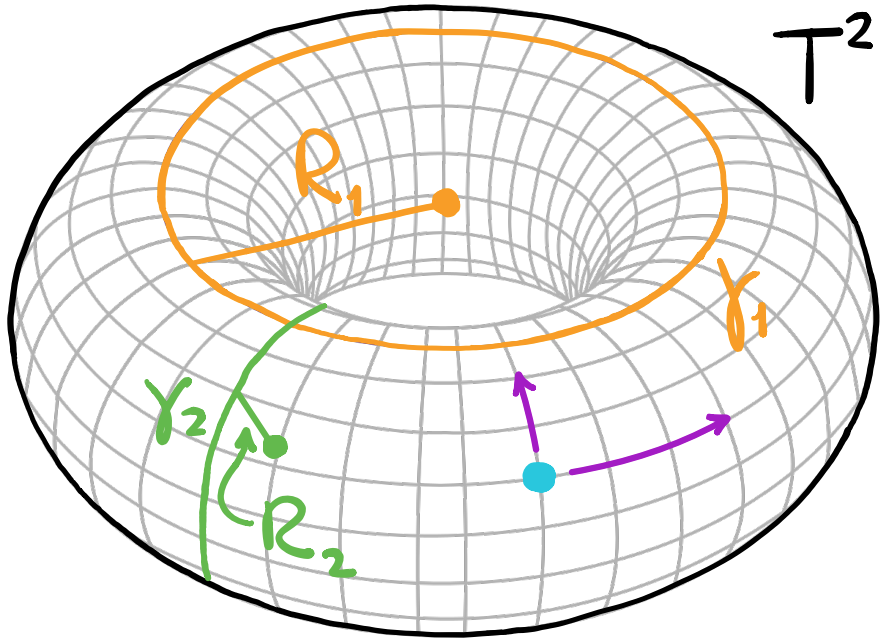
\includegraphics[width=0.5\textwidth]{figures/fig2_anyon_torus.png}
  \caption{一个在环面上运动的任意子。（原文 Figure 2，原文 p.10）}
  \label{fig:torus}
\end{figure}

% 原文标题：Canonical quantization.
\paragraph{正则量子化}规范理论的正则量子化分三步：(1) 固定一个规范，以施加规范不变性；(2) 施加所有非动力学约束；(3) 把正则泊松括号提升为对易子。这三步的先后不影响所得的量子理论；但（依理论而定）选错次序会带来难以逾越的困难。在目前的情形，我们从作用量 \eqref{eq:2.20} 出发，取 $A_0 = 0$ 规范，得到 \eqref{eq:2.22}。这一步等同于在作用量中施加约束 $F_{12} = 0$；不过须记住：高斯定律要在整个相空间上实施。在此阶段，运动方程的解仍未受约束，即它们可以有 $F_{12} = \partial_1A_2 - \partial_2A_1 \neq 0$。

这里我们选择先量子化、后施加约束：这一策略可行，因为运动方程与约束都对 $A$ 线性。在 \S\ref{sec:4} 中，我们会在高斯定律非线性的情形下采取相反的策略。
% ==== 原文 p.11 ====
正则泊松括号可直接从 \eqref{eq:2.22} 读出，随后把 $A_i$ 提升为算符：
\begin{equation}\tag{2.23}\label{eq:2.23}
  \{A_i(\mathbf x), A_j(\mathbf y)\}
  = \frac{2\pi}{k}\varepsilon_{ij}\delta^{(2)}(\mathbf x-\mathbf y)
  \ \rightsquigarrow\
  [A_i(\mathbf x), A_j(\mathbf y)]
  = \left(\frac{2\pi i}{k}\right)\varepsilon_{ij}\delta^{(2)}(\mathbf x-\mathbf y).
\end{equation}

% [Tutor Note: 易错点] 泊松括号换对易子要乘 i；(2.23) 的 ε_{ij} 与 (2.20) 的 ε^{ij} 混用上下标，不改符号
\begin{yizhu}[易错点]
正则量子化的替换规则是 $[\,\cdot\,,\cdot\,] = i\{\,\cdot\,,\cdot\,\}$，所以 \eqref{eq:2.23} 左式的 $2\pi/k$ 变成右式的 $2\pi i/k$：$i$ 只出现在对易子一侧，$k$ 仍在分母。又，此式两处都写 $\varepsilon_{ij}$（下标），而 \eqref{eq:2.20}、\eqref{eq:2.22} 用 $\varepsilon^{ij}$ 配 $A_i$；2 维空间里 $\varepsilon^{12}=\varepsilon_{12}=+1$，数值不变。这是作者混用上下标的习惯，不能据此补负号。
\end{yizhu}

% 原文标题：Solving the theory.
\paragraph{求解理论}现在来定基态波泛函 $\Psi_0[A(x)]$。这在场论中几乎做不到；不过在 $A_0 = 0$ 规范下 CS 作用量是二次的——理论自由——所以我们预期基态为高斯型。出于凝聚态理论中朗道能级的启发\footnote{另一种说法是：$A_0 = 0$ 规范把物理约化到平面 $\R^2 = \C$ 上，那里复坐标随手可得。\S\ref{sec:4} 关于全纯量子化的讨论也将呼应并拓展这一想法。}（见 \cite{dunne}），我们采用复坐标：
\begin{equation}\tag{2.24}\label{eq:2.24}
  z = x_1 + i x_2, \qquad A = A(z) = \sqrt{\frac{k}{2\pi}}\,(A_1 + iA_2).
\end{equation}
我们为基态取如下拟设，希望把它显式定出来：
\begin{equation}\tag{2.25}\label{eq:2.25}
  \Psi_0[A,\bar A] = \Psi[A(z)]\exp\left(-\frac12\int |A|^2\right).
\end{equation}
现在必须把 $F_{12} = 0$ 作为希尔伯特空间上的泛函方程施加。为此，先把对易子 \eqref{eq:2.23} 用重标度后的场 $A$ 与 $\bar A$ 改写，得到 $[A(z),\bar A(w)] = \delta(z-w)$。于是我们有权把 $A$ 看作“$x$”、把 $i\bar A$ 看作“$p$”，仿照量子力学写下 $\bar A = -\delta/\delta A$。这样 $F_{12} = \partial_1A_2 - \partial_2A_1$ 成了一个微分算子，可按（反）全纯导数 $\partial_\pm = \partial_1\mp i\partial_2$ 重新组织：
\begin{equation}\tag{2.26}\label{eq:2.26}
  F_{12}\Psi_0[A,\bar A]
  = \left(\partial_-\,\frac{\delta}{\delta A} + \partial_+A\right)\Psi_0[A,\bar A] = 0
  \quad\Longrightarrow\quad
  \left(\partial_-\,\frac{\delta}{\delta A} + \partial_+A\right)\Psi[A(z)] = 0.
\end{equation}
因子 $e^{-\frac12\int|A|^2}$ 消去，所得关于 $\Psi[A(z)]$ 的方程有高斯解：
\begin{equation}\tag{2.27}\label{eq:2.27}
  \Psi[A] \sim \exp\left[-\frac12\int A\left(\frac{\partial_+}{\partial_-}\right)A\right]
  \quad\Longrightarrow\quad
  \Psi_0[A(z)] = \exp\left(-\frac12\int\left[A\left(\frac{\partial_+}{\partial_-}\right)A + |A|^2\right]\right).
\end{equation}

% [Tutor Note: 易错点] (2.24) 的归一化：由 √(k/2π) 与 (2.23) 算得 [A,Ā]=2δ，与下文 [A,Ā]=δ(z−w) 差因子 2
\begin{yizhu}[易错点]
取 \eqref{eq:2.24} 的 $A=\sqrt{k/2\pi}\,(A_1+iA_2)$，代 \eqref{eq:2.23} 直接算得 $[A(z),\bar A(w)] = \frac{k}{2\pi}(-2i)\frac{2\pi i}{k}\delta^{(2)}(\mathbf x-\mathbf y) = 2\delta^{(2)}(\mathbf x-\mathbf y)$，而 \eqref{eq:2.26} 前原文写 $[A(z),\bar A(w)] = \delta(z-w)$。若约定 $\delta(z-w)=\delta^{(2)}(x-y)$，两式差因子 2；要让 $[A,\bar A]=\delta(z-w)$ 成立，\eqref{eq:2.24} 的 $2\pi$ 应换成 $4\pi$。作者随即用 $\bar A=-\delta/\delta A$，这套写法只与 $[A,\bar A]=\delta$ 配套；此处按原文的约定读，勿再乘 2。
\end{yizhu}

% [Tutor Note: 易错点] (2.26) 的 Ā=−δ/δA：符号由 [A,Ā]=δ 定死；∂± 定义不带 1/2
\begin{yizhu}[易错点]
$\bar A$ 在 \eqref{eq:2.26} 里实现为 $-\delta/\delta A$，地位等同量子力学中的 $p=-i\partial_x$：由 $[\delta/\delta A, A] = 1$ 得 $[A,-\delta/\delta A] = +\delta$；若漏掉负号，算符 \eqref{eq:2.26} 与高斯解 \eqref{eq:2.27} 会同时反号。另注意原文定义 $\partial_\pm = \partial_1\mp i\partial_2$ 不带 $\frac12$，与标准的 $\partial_z=\frac12(\partial_1-i\partial_2)$ 差因子 2；\eqref{eq:2.27} 中 $\partial_+/\partial_-$ 按原定义读，并记住它是形式算符之比。
\end{yizhu}

% [Tutor Note: 含糊点] 作者说 e^{−½∫|A|²} “drops out”，但 (2.27) 方括号里仍留 |A|²：它是被配方吸收的
\begin{yizhu}[含糊点]
作者称因子 $e^{-\frac12\int|A|^2}$ “drops out”，但 \eqref{eq:2.27} 的方括号里仍留着 $+|A|^2$：它并未消失，而是与高斯型解合并（配方）了。要从 \eqref{eq:2.26} 走到 \eqref{eq:2.27}，须把 $\bar A$ 实现为 $-\delta/\delta A$、把 $\partial_+/\partial_-$ 当成形式算符比，并处理二次型核的对称化；作者省略了这步代数。可对照 \cite{dunne} 的朗道能级波函数与 \cite{woodhouse} 的全纯量子化处理。
\end{yizhu}

% 原文标题：The torus again.
\paragraph{又见环面}前面我们研究过纯 CS 理论在环面上的经典相空间。现在手头有了对易子 \eqref{eq:2.23}，就可以量子化威尔逊圈了。我们写下 $W_a = e^{iw_a}$，其中 $w_a = \oint_{\gamma_a}\dd x^\mu_a A_\mu$。取 $A_0 = 0$ 规范，代入正则对易子 \eqref{eq:2.23} 并积分，得到 $[w_1,w_2] = \frac{2\pi i}{k}$。BCH 公式给出 $W_1$ 与 $W_2$ 所服从的代数：$W_1W_2 = e^{2\pi i/k}W_2W_1$。这一代数最小的非平凡表示维数为 $k\in\Z$，所以处在该表示中的场给出 $k$ 重基态简并。在亏格 $g$ 的曲面上，威尔逊圈更多；相应的代数也更复杂，基态简并度增长为 $k^g$。这种简并是新型拓扑物相的一个标志。

% [Tutor Note: 易错点] [w₁,w₂]=2πi/k 与 W₁W₂=e^{2πi/k}W₂W₁ 须配套：BCH 给出 e^{−2πi/k}，差号源于圈定向
\begin{yizhu}[易错点]
由 \eqref{eq:2.23} 沿两条生成圈积分得 $[w_1,w_2]=2\pi i/k$。再用 BCH：$e^{iw_1}e^{iw_2}=e^{i(w_1+w_2)}e^{-\frac12[w_1,w_2]}$，于是 $W_1W_2=e^{-2\pi i/k}W_2W_1$，与原文的 $e^{+2\pi i/k}$ 差一个符号。差异出在两条生成圈 $\gamma_1,\gamma_2$ 的定向（交点符号为 $\pm1$）；原文没有指定定向，故两式只能成套使用，不能各取一半。
\end{yizhu}

% [Tutor Note: 含糊点] “最小非平凡表示维数为 k”的理由：取 W₁^k W₂ 的迹得 ω^k=1，clock–shift 表示维数 k
\begin{yizhu}[含糊点]
作者直接断言“最小非平凡表示的维数为 $k\in\Z$”。理由：记 $\omega = e^{2\pi i/k}$，由 $W_1W_2 = \omega W_2W_1$ 得 $W_1^kW_2 = \omega^kW_2W_1^k$，两边取迹即要求 $\omega^k = 1$，故有限维表示只在 $k$ 为整数时存在；其不可约表示由时钟矩阵与移位矩阵给出，维数恰为 $k$，于是有 $k$ 重简并。亏格 $g$ 时每个把手贡献一对圈，简并度为 $k^g$。可参 \cite{witten1989} 与 \cite{verlinde1988}。
\end{yizhu}

% ==== 原文 p.12 ====

\subsection{拓扑学的锦上添花}\label{sec:2.4}
% 原文标题：Topological Bells and Whistles

% 原文标题：An invariant perspective.
\paragraph{不变量视角}看看无坐标的表述能为 CS 理论做点什么。先把 CS 作用量 \eqref{eq:2.1} 用微分形式重写：
\begin{equation}\tag{2.28}\label{eq:2.28}
  \SCS = \frac{k}{4\pi}\int_M A\wedge\dd A, \qquad A = A_\mu\dd x^\mu \in \Omega^1(M).
\end{equation}
CS 3-形式 $A\wedge\dd A$ 可定义在任何可定向 3-流形 $M$ 上，无需引用度规。它的积分是 $M$ 的拓扑不变量，尤其它在任意坐标变换下不变。如同在引力中那样，我们把坐标变换看作规范对称性。其中之一正是时间流动本身：相应的诺特荷——哈密顿量——必须恒等于零，这印证了 \S\ref{sec:2.3} 的正则分析。此外，$\SCS$ 不依赖度规，于是整个能动张量都为零：
\begin{equation}\tag{2.29}\label{eq:2.29}
  T^{\mu\nu}_{\mathrm{CS}} = \frac{2}{\sqrt{|g|}}\frac{\delta\mathcal{L}_{\mathrm{CS}}}{\delta g_{\mu\nu}} = 0.
\end{equation}
CS 理论与引力都具备这些特征——微分同胚不变性与 $H = 0$。事实上，3 维引力有一个一阶表述，就是一个 CS 理论 \cite{achucarro1986}！

% [Tutor Note: 物理图像] 作用量不含度规，便没有局部能动张量；H=0 即拓扑场论的定义性特征
\begin{yizhu}[物理图像]
作用量里没有度规，就无从对度规变分，能动张量只能为零：理论没有传播的局部自由度，能标出“物理”的只有拓扑。$H = 0$ 同理——时间平移本身是规范变换，所以没有能量，也就没有演化。这正是拓扑场论区别于普通场论的地方。
\end{yizhu}

% 原文标题：The θ term.
\paragraph{$\theta$ 项}微分形式的好处之一，是它澄清了 $\SCS$ 与 4 维杨–米尔斯理论中 $\theta$ 项的关系。主要想法 \cite{tong_gauge} 是把 $M$ 看成某个 4-流形 $X$ 的边界，再用斯托克斯定理与 $F = \dd A$ 写下
\begin{equation}\tag{2.30}\label{eq:2.30}
  S^{X}_{\mathrm{CS}}
  = \frac{k}{4\pi}\int_{\partial X} A\wedge\dd A
  = \frac{k}{4\pi}\int_X F\wedge F
  = \frac{k}{2\pi}\int_X \dd^4x\,F^{MN}\widetilde{F}_{MN} .
\end{equation}
这里我们在 $X$ 上给定一个度规，并用 $\widetilde{F}^{MN} = \frac12\varepsilon^{MNAB}F_{AB}$ 写出 $F\wedge F$ 的分量。（等价地，$F\wedge F$ 的积分就是 2-形式的霍奇内积 $\langle F,\star F\rangle$。）于是在整体归一化之内，CS 作用量就是一个 $\theta$ 项。

% [Tutor Note: 原文疑误] (2.30) 末项系数：k/4π∫F∧F = k/8π∫F^{MN}F̃_{MN}，原文写 k/2π，大 4 倍
\begin{yizhu}[原文疑误]
按 $F=\frac12F_{MN}\dd x^M\wedge\dd x^N$ 展开，$F\wedge F=\frac14\varepsilon^{MNAB}F_{MN}F_{AB}\dd^4x$；而 $\widetilde F^{MN}=\frac12\varepsilon^{MNAB}F_{AB}$ 给出 $F^{MN}\widetilde F_{MN}=\frac12\varepsilon^{MNAB}F_{MN}F_{AB}$，故 $\frac{k}{4\pi}\int F\wedge F=\frac{k}{8\pi}\int\dd^4x\,F^{MN}\widetilde F_{MN}$。\eqref{eq:2.30} 末一项写 $k/2\pi$，比正确系数大 4 倍。此处照录原文；\eqref{eq:2.31} 用的仍是 $k/4\pi$ 形式，故整性判据的结论不受影响。
\end{yizhu}

% 原文标题：Spin manifolds.
\paragraph{自旋流形}从 4 维视角看，$\SCS$ 只依赖 $F$，规范不变性是显然的。然而它现在关键地依赖我们对“体”时空 $X$ 的选择，而这不能成立。为使理论良定义，我们要求：任意两个有公共边界 $\partial X = \partial X' = M$ 的 4-流形 $X$、$X'$ 都满足 $S^{X}_{\mathrm{CS}} - S^{X'}_{\mathrm{CS}} \in 2\pi\Z$，以保持 \eqref{eq:2.12} 式的配分函数。重述这一判据的巧妙办法，是引入紧致 4-流形 $Y = (X\cup X')/M$：把 $X$ 与 $X'$ 沿公共边界 $M$ 以反转定向的方式粘起来。于是我们的要求读作
\begin{equation}\tag{2.31}\label{eq:2.31}
  S^{X}_{\mathrm{CS}} - S^{X'}_{\mathrm{CS}}
  = \frac{k}{4\pi}\int_Y F\wedge F \stackrel{!}{=} 2\pi n,
  \qquad n\in\Z.
\end{equation}
% ==== 原文 p.13 ====
结果表明，这一整性条件只在 $Y$ 是自旋流形时才成立；所谓自旋流形，就是能承载旋量的流形。例如 $T^4$、$S^4$ 与 $S^2\times S^2$ 都是自旋流形，而 $\mathbb{CP}^2$ 不是。至此，我们用几何解决了一个拓扑问题，并认识到：3 维 CS 理论与带费米子的 4 维规范理论有着内在联系。

% [Tutor Note: 含糊点] 整性只在自旋流形上成立：∫F∧F/4π² 为整数，自旋 4-流形相交形式为偶
\begin{yizhu}[含糊点]
作者称整性条件“只在 $Y$ 是自旋流形时成立”，未给证明。依据是：对 $\mathrm{U}(1))$ 丛，$\frac{1}{4\pi^2}\int_Y F\wedge F = \int c_1^2$ 为整数；自旋 4-流形的相交形式为偶（$w_2(Y)=0$ 的经典推论），故该整数为偶数 $2n$，于是 $\frac{k}{4\pi}\int F\wedge F = 2\pi kn$ 自动落在 $2\pi\Z$ 内。非自旋的 $\mathbb{CP}^2$ 相交形式为奇，只有偶数 $k$ 才相容。可参 \cite{witten1989} 与 \cite{aps1975}。
\end{yizhu}

% =============================================================================
% 汇报（供 Lead 汇总）
% 片段：2.3–2.4，原文 p.9–13
% 编号公式：(2.20)–(2.31) 共 12 个，均以 \tag 锁定；无编号展示公式：无
% 图 2 一处（fig:torus，p.10）；脚注 3 一处（p.11）
% 译注 10 条：易错点 5、含糊点 3、物理图像 1、原文疑误 1
% (2.30) 因子裁定：确认 SPEC §10 第 4 条成立。按 F=½F_{MN}dx^M∧dx^N 得
%   F∧F=¼ε^{MNAB}F_{MN}F_{AB}d^4x，而 F̃^{MN}=½ε^{MNAB}F_{AB}，故
%   (k/4π)∫F∧F=(k/8π)∫d^4x F^{MN}F̃_{MN}；原文末项写 k/2π，大 4 倍（4×k/8π）。
%   正文照录，已加「原文疑误」译注。(2.31) 仍用 k/4π 形式，结论不受影响。
% 其他核对结果：
%   1) (2.20)：由 (2.1) 按 ε^{012}=+1 展开，动能项应为 −ε^{ij}A_i\dot A_j，原文写 +；
%      与 (2.4)/(2.6) 定出的 ε^{0ij}=ε^{ij} 对照，仅动能项整体反号。作者以 (2.22)
%      的 L 定 (2.23)，故照录 + 批注（易错点）。SPEC §10 未列此条。
%   2) (2.24) 归一化：按 √(k/2π) 与 (2.23) 算得 [A,Ā]=2δ^{(2)}，原文下一段写
%      [A,Ā]=δ(z−w)，疑差因子 2（要自洽宜取 √(k/4π)）。照录 + 批注，存疑待裁定。
%   3) 环面：[w1,w2]=2πi/k 与 W1W2=e^{2πi/k}W2W1 依 BCH 差一符号，源自圈定向未定义；
%      照录 + 批注（SPEC §10 第 3 条的核对结论）。
%   4) p.11 提取文本 "correponding" 经图像核对为 "corresponding"，非笔误，不批注。
%   5) 跨片段引用：\eqref{eq:2.1}、\eqref{eq:2.4}、\eqref{eq:2.6}、\eqref{eq:2.12}、
%      \S\ref{sec:2.2}、\S\ref{sec:4}（需 s02a / s04a 的 label 与之一致）。
%   6) 段落：原文跨页处（p.9→p.10 尾句、p.10→p.11 "Poisson brackets"、p.12→p.13）
%      保持同段不断开，锚点注在段内相应位置。
% 自检：python tools/lint.py sections/s02b-abelian2.tex --tags 2.20,...,2.31 -> OK
% =============================================================================
% >>>>>>>>>>>>>>>> end sections/s02b-abelian2.tex <<<<<<<<<<<<<<<<

% >>>>>>>>>>>>>>>> sections/s03a-framing.tex <<<<<<<<<<<<<<<<
% =============================================================================
%  s03a-framing.tex —— 第 3 节「标架化与路径积分」：标题、引言、3.1、3.2
%  覆盖原文 p.13（"Apologia for geometry."）至 p.19 式 (3.24)；编号公式 (3.1)–(3.24)
% =============================================================================

% ==== 原文 p.13 ====
\section{标架化与路径积分}\label{sec:3}

% [Tutor Note: 本节重点] 物理图像/数学工具/主要结论
\begin{keytakeaways}
\begin{itemize}[leftmargin=1.4em,itemsep=2pt,topsep=2pt]
  \item \textbf{物理图像：}非阿贝尔陈--西蒙斯作用量在规范变换下只差 $2\pi k\,w(g)$；绕数非零的大规范变换迫使能级 $k$ 取整数，量子理论靠振幅 $e^{i\SCS}$ 的单值性存活。
  \item \textbf{数学工具：}主 $G$-丛上的联络与曲率 $F=\dd A+A\wedge A$、博特定理 $\pi_3(G)=\Z$、法捷耶夫--波波夫规范固定、一圈行列式 $\det(\Delta)/\sqrt{\det(L_-)}$，以及阿蒂亚--帕托迪--辛格指标定理给出的 $\eta$ 相位。
  \item \textbf{主要结论：}大 $k$ 下配分函数由平坦联络的稳相求和给出：$\mathcal{Z}=e^{i\pi\eta[0]/2}\sum_\alpha e^{i(k+c_2(G)/2)I[A^{(\alpha)}]}T_\alpha$，能级平移 $k\to k+c_2(G)/2$ 在此出现。
\end{itemize}
\end{keytakeaways}

\paragraph{为几何辩护}
% 原文标题：Apologia for geometry.
上一节我们刻意保持朴素，选择了初等、却未必深刻的表述方式。现在，某种意义上要一切从头再来。这一回的叙述会明显更形式化，但这里发展出的几何始终由阿贝尔理论中积累的直觉引导。此前遇到的全部现象，如今都要配上纤维、丛与表示，抽象地铺展开来。我们先完整地建立非阿贝尔陈--西蒙斯（CS）理论，给出它在规范变换下的行为，再用纽结描述它的物理可观测量（威尔逊圈）。随后转向大 $k$ 下配分函数的鞍点计算；此时理论弱耦合。为正规化过程中出现的那些相当微妙的发散，我们将讨论定向 3-流形与纽结的标架化。最后，弄清路径积分在标架变换下如何变化，就能完成这些计算。

\subsection{非阿贝尔陈--西蒙斯作用量}\label{sec:3.1}

\paragraph{几何设定}
% 原文标题：Geometrical setting.
故事始于一个代表时空的定向 3-流形 $M$，以及一个紧致单李群 $G$——规范群，其李代数为 $\mathfrak{g}$。作为物理学家，我们有时把李群与它的李代数混为一谈。这里我们虽努力区分 $G$ 与 $\mathfrak{g}$，却难免仍有不精确之处。为使规范变换的概念严格化，固定一个主 $G$-丛\footnote{为方便起见，可以设想 $E=M\times G$ 是平凡丛，取 $M=S^3$、$G=\mathrm{SU}(N)$。我们的形式适用于更一般的情形，但这是遇到困难时值得回头参考的有用例子。} $E\to M$。$E$ 的截面称为规范变换，它们是映射 $g\colon M\to E$，把每个 $x\in M$ 光滑地对应到一点 $g(x)=(x,g_x)\in E$，其中 $g_x\in G$。我们常滥用记号，写成 $g(x)=g_x$，把 $g$ 看作映射 $M\to G$，给出依赖时空位置的 $G$ 元素。当 $g_x$ 接近 $G$ 的单位元时，我们改而考虑无穷小（生成元形式的）规范变换，并把 $g(x)$ 视为 $\mathfrak{g}$ 值的零形式，即依赖时空位置的李代数生成元。

接下来，在 $E$ 上引入主联络。在物理学家看来，\footnote{关于恰当的数学表述（包括伴丛方面的洞见），参见 \cite{steenrod1951} 或 \cite{nakahara}。} 它不过是 $M$ 上一个取 $\mathfrak{g}$ 值的 1-形式。记该联络为 $A$；在 $M$ 的局部坐标下写 $A=A_\mu(x)\dd x^\mu$。每个 $A_\mu(x)$ 都落在李代数里，因此给定 $\mathfrak{g}$ 的一组基 $T^a$，还可分解 $A_\mu(x)=A^a_\mu(x)T^a$，其中规范指标 $a\in\{1,\dots,d=\dim G\}$。这个对象 $A_\mu(x)$ 称为规范场，它推广了 \S\ref{sec:2} 的 $\mathrm{U}(1)$ 规范场。现在可以问一个自然的问题：既然 $E$ 自带 $G$ 作用，

% ==== 原文 p.14 ====
联络在该作用下如何变化？换句话说，规范场在规范变换下如何改变？答案就是下述变换律：
\begin{equation}\tag{3.1}\label{eq:3.1}
  A_\mu \longrightarrow A'_\mu = g^{-1}A_\mu g + g^{-1}\partial_\mu g,
  \qquad g = g(x)\in E.
\end{equation}

\paragraph{协变导数与曲率}
% 原文标题：Covariant derivative and curvature.
为得到该变换律的无穷小版本，引入规范协变导数 $D$。它作用在 $\mathfrak{g}$ 值微分形式 $\omega$ 上，$D_\mu\omega=\partial_\mu\omega+[A_\mu,\omega]$，其中 $[\cdot,\cdot]$ 是李括号。在局部规范变换 $\varepsilon(x)\in\Omega^0(M,\mathfrak{g})$ 下，规范场按协变导数改变：$A_\mu\to A_\mu-D_\mu\varepsilon$。用行话说，联络通过 $[A_\mu,\cdot]$ 把普通导数 $\partial_\mu$“扭”了一下。要考察 $A_\mu$ 引入了多少扭曲，可以测量 $D_\mu$ 与自身不对易的程度；若规范丛平坦，$D_\mu$ 本应对易。因此，我们如下定义联络的曲率，也称场强：
\begin{equation}\tag{3.2}\label{eq:3.2}
  F_{\mu\nu} \equiv [D_\mu, D_\nu] = \partial_\mu A_\nu - \partial_\nu A_\mu + [A_\mu, A_\nu]
  \quad\Longleftrightarrow\quad F = \dd A + A\wedge A.
\end{equation}

% [Tutor Note: 易错点] (3.2) 分量式中 [A_μ,A_ν] 的系数是 1 不是 1/2；形式式 F=dA+A∧A 里那 1/2 已被 A∧A 的反对称化吸收，两套写法不可重复记账。
\begin{yizhu}[易错点]
\eqref{eq:3.2} 的分量式里 $[A_\mu,A_\nu]$ 的系数是 $1$，不是 $1/2$。用形式记号写就是 $F=\dd A+A\wedge A$；分量式里的 $[A_\mu,A_\nu]$ 与形式式里的 $A\wedge A$ 只差一次反对称化，那个 $1/2$ 已经并进 $A\wedge A$ 里。反过来，从形式式走到分量式 $F_{\mu\nu}=\partial_\mu A_\nu-\partial_\nu A_\mu+[A_\mu,A_\nu]$ 时，切不可再补一个 $1/2$。这个定义还与协变导数 $D_\mu\omega=\partial_\mu\omega+[A_\mu,\omega]$ 绑定：若改用厄米约定写 $A$，$[A_\mu,A_\nu]$ 前的符号也要随之改，否则 $[D_\mu,D_\nu]$ 展不出来。
\end{yizhu}

若 $G$ 阿贝尔（例如 $G=\mathrm{U}(1)$），则所有对易子为零。此时 $D_\mu=\partial_\mu$，$F_{\mu\nu}$ 化为通常的麦克斯韦场强张量。但非阿贝尔场强含有 $A$ 的二次项，一般是非线性的。若 $F=0$，则称联络 $A$ 平坦。受 \eqref{eq:2.2} 启发，我们很快会看到：$E$ 上平坦联络的空间决定纯陈--西蒙斯理论的经典相空间。

\paragraph{陈--西蒙斯作用量}
% 原文标题：The Chern--Simons action.
从 $A$ 出发，我们如下定义陈--西蒙斯作用量：
\begin{equation}\tag{3.3}\label{eq:3.3}
\begin{aligned}
  \SCS[A] &\equiv \frac{k}{4\pi}\int_M \Tr\Bigl(A\wedge\dd A + \frac{2}{3}A\wedge A\wedge A\Bigr)\\
  &= \frac{k}{4\pi}\int_M \dd^3x\,\varepsilon^{\mu\nu\rho}\Tr\Bigl(A_\mu(\partial_\nu A_\rho - \partial_\rho A_\nu) + \frac{2}{3}A_\mu[A_\nu,A_\rho]\Bigr).
\end{aligned}
\end{equation}

% [Tutor Note: 原文疑误] (3.3) 第二行比第一行恰大一倍：A∧dA=½εA(∂νAρ−∂ρAν)、A∧A∧A=½εA[Aν,Aρ]，故括号前应有整体 ½，系数应为 1/2 与 1/3；且与 (3.4) 的 1/3 自相矛盾。
\begin{yizhu}[原文疑误]
按形式式展开，$\dd^3x\,\varepsilon^{\mu\nu\rho}$ 前应带整体 $\frac12$：$A\wedge\dd A=\frac12\varepsilon^{\mu\nu\rho}A_\mu(\partial_\nu A_\rho-\partial_\rho A_\nu)$，$A\wedge A\wedge A=\frac12\varepsilon^{\mu\nu\rho}A_\mu[A_\nu,A_\rho]$。照此，\eqref{eq:3.3} 第二行括号内的系数应是 $\frac12$ 与 $\frac13$，原文却写成 $1$ 与 $\frac23$，整行恰为第一行的两倍。旁证是 \eqref{eq:3.4} 与 \eqref{eq:3.5}：那里 $\frac13$ 与 $1/24\pi^2$ 配套得出 $\Delta\SCS=2\pi k\,w(g)$，只有按第一行解释才自洽。中译本照录原文，不作改动。
\end{yizhu}

$\mathfrak{g}$ 值的 3-形式 $\omega_{\mathrm{CS}}\equiv A\wedge\dd A+\frac23 A\wedge A\wedge A$ 就是著名的陈--西蒙斯形式；这里的 $\Tr$ 指 $\mathfrak{g}$ 上基灵型的某个倍数（归一化稍后确定）。更具体地说，在 $\mathfrak{g}$ 的伴随表示中，$\omega_{\mathrm{CS}}$ 不过是一个（由 3-形式组成的）矩阵，而这个矩阵的迹正比于 $\Tr(\omega)$。由 \eqref{eq:3.3} 得出的运动方程，来自场变分 $\delta A$ 所引起的 $\delta\SCS$，即 $\delta\SCS=0\Longrightarrow F^a_{\mu\nu}=0$。正如许诺的那样，这描述了 $E$ 上平坦联络的空间。

% [Tutor Note: 易错点] δS_CS=(k/2π)∫Tr(δA∧F) 只是体项；M 带边界时还有 (k/4π)∫_{∂M}Tr(A∧δA)，作者写 δS_CS=0\$\\ 即默认边界项消失。
\begin{yizhu}[易错点]
$\delta\SCS=0\Longrightarrow F=0$ 这一步默认了边界项消失。直接变分给出 $\delta\SCS=\frac{k}{2\pi}\int_M\Tr(\delta A\wedge F)$，再加边界项 $\frac{k}{4\pi}\int_{\partial M}\Tr(A\wedge\delta A)$；只有 $M$ 无边界，或限定 $\delta A$ 在 $\partial M$ 上为零，才能把后者丢掉而得到 $F^a_{\mu\nu}=0$。作者下文说全散度项“加上适当的边界条件”即消失，用的正是同一默认，但此处没有明说。
\end{yizhu}

% [Tutor Note: 易错点] (3.3) 的 2/3 与 Tr 归一化互相锁定：取基础表示 Tr(T^aT^b)=δ^{ab}/2，才有 (3.4)-(3.5) 的 ΔS=2πkw 与 w(g)∈Z。
\begin{yizhu}[易错点]
\eqref{eq:3.3} 中的 $\frac23$ 与 $\Tr$ 的归一化要分开看、配套用。$\frac23$ 这个系数保证作用量在规范变换下只差一个全导数，再加一项正比于 $\int\varepsilon^{\mu\nu\rho}\Tr(g^{-1}\partial_\mu g\,g^{-1}\partial_\nu g\,g^{-1}\partial_\rho g)$ 的量；$\Tr$ 的倍数则决定后者的数值：取基础表示 $\Tr(T^aT^b)=\frac12\delta^{ab}$ 时，\eqref{eq:3.5} 的 $w(g)$ 恰为整数，\eqref{eq:3.4} 的 $\frac13$ 与之配套给出 $\Delta\SCS=2\pi k\,w(g)$。若改取 $\Tr(T^aT^b)=\delta^{ab}$，$w(g)$ 整体翻倍，$1/24\pi^2$ 也得跟着改。作者随后正是拿“$w(g)$ 恰为整数”反过来定 $\Tr$ 的倍数。
\end{yizhu}

\paragraph{能级的量子化}
% 原文标题：Quantization of the level.
呼应 \S\ref{sec:2.2}，我们要问：陈--西蒙斯作用量 \eqref{eq:3.3} 在规范变换 \eqref{eq:3.1} 下是否不变？一次简短的分部积分练习给出
\begin{equation}\tag{3.4}\label{eq:3.4}
  \delta\SCS = \frac{k}{4\pi}\int_M \dd^3x\,\varepsilon^{\mu\nu\rho}\Bigl(\partial_\mu\Tr\bigl[(\partial_\nu g)(g^{-1}A_\rho)\bigr] + \frac{1}{3}\Tr\bigl[(g^{-1}\partial_\mu g)(g^{-1}\partial_\nu g)(g^{-1}\partial_\rho g)\bigr]\Bigr).
\end{equation}

% ==== 原文 p.15 ====
第一项是熟悉的全散度 \eqref{eq:2.10} 的乔装；与阿贝尔情形一样，只要加上适当的边界条件，它就消失。第二项是非阿贝尔理论的新东西，与一个称为 $g$ 的绕数的积分有关：
\begin{equation}\tag{3.5}\label{eq:3.5}
  w(g) \equiv \frac{1}{24\pi^2}\int_M \dd^3x\,\varepsilon^{\mu\nu\rho}\Tr\bigl[(g^{-1}\partial_\mu g)(g^{-1}\partial_\nu g)(g^{-1}\partial_\rho g)\bigr] = (\text{constant})\cdot n,
  \quad n\in\Z.
\end{equation}

% [Tutor Note: 易错点] (3.4) 的 1/3 与 (3.5) 的 1/24π² 必须配套：ΔS=(k/4π)(1/3)∫εTr=2πk·w，故 k∈Z 才是单值条件；任一系数改动都会破坏这一配对。
\begin{yizhu}[易错点]
\eqref{eq:3.4} 的 $\frac13$ 与 \eqref{eq:3.5} 的 $1/24\pi^2$ 是一对，不能分开改：规范变换后 $\Delta\SCS=\frac{k}{4\pi}\cdot\frac13\int_M\dd^3x\,\varepsilon^{\mu\nu\rho}\Tr\bigl[(g^{-1}\partial_\mu g)(g^{-1}\partial_\nu g)(g^{-1}\partial_\rho g)\bigr]=\frac{k}{12\pi}\int\cdots=2\pi k\,w(g)$。正因 $w(g)$ 取整数，振幅 $e^{i\SCS}$ 的单值性才归结为 $k\in\Z$。若把 $\frac13$ 改成别的数，$2\pi k\,w(g)$ 的整倍数结构就断了；\eqref{eq:3.3} 第二行那个差一倍的写法正是这种断裂的旁证。
\end{yizhu}

$w(g)$ 的量子化在瞬子研究中广为人知（证明见 \cite{coleman}）。因此我们固定 $\Tr$ 的归一化，使 $w(g)$ 恰为整数。用 $w(g)$ 表示，陈--西蒙斯作用量在规范变换下改变一个常数：$\SCS\to\SCS+2\pi k\,w(g)$。$w(g)=0$ 的变换保持 $\SCS$ 不变，$w(g)\neq0$ 的变换则不然。绕数非零的 $g(x)$ 称为大规范变换（large gauge transformation），它们非平凡地“缠绕” $G$。这类变换使经典陈--西蒙斯理论定义不良；但依 \S\ref{sec:2.2} 的论证，只要振幅 $e^{-\SECS}=e^{i\SCS}$ 单值，量子理论仍然自洽。这就要求 $2\pi k\,w(g)$ 为整数，从而 $k\in\Z$。

% [Tutor Note: 原文疑误] 「2πkw(g) 为整数」字面不成立：单值性要求 e^{2πikw}=1，即 k w(g)∈Z；结论 k∈Z 不变
\begin{yizhu}[原文疑误]
原文此句作 “This forces $2\pi k\,w(g)$ to be an integer”，字面读不通：$e^{i\SCS}$ 单值只要求 $e^{2\pi ik\,w(g)}=1$，即 $k\,w(g)\in\Z$，等价于说 $2\pi k\,w(g)$ 是 $2\pi$ 的整数倍，而不是它本身为整数（后者对一般的 $k$ 无解）。取 $w(g)=1$ 即得 $k\in\Z$，故结论不受影响。中译本照录原文措辞，读者按 $e^{2\pi ik\,w}=1$ 理解即可。
\end{yizhu}

\paragraph{规范变换的拓扑}
% 原文标题：Topology of gauge transformations.
$w(g)$ 的出现看似奇迹，其实是 $G$ 拓扑的推论。回忆：规范变换是映射 $g\colon M\to G$，$x\mapsto g(x)$。其中包含恒等映射 $x\mapsto 1_G$。人们可以问：是否所有规范变换都与恒等映射同伦（即可连续形变到恒等映射）？答案是否定的。例如取 $M=S^3$，映射 $g\colon S^3\to G$ 的集合由群 $\pi_3(G)$ 分类；博特（Bott）\cite{bott1956} 有一个著名结果：对每个紧致单李群 $G$，$\pi_3(G)=\Z$。

% [Tutor Note: 含糊点] π3(G)=Z 只引 Bott [12] 而不证：这是 Bott 用 Morse 理论研究紧李群拓扑的结论，生成元可取 S³≅SU(2)⊂G 的嵌入，其绕数正是 (3.5) 的 WZW 整数。
\begin{yizhu}[含糊点]
“$\pi_3(G)=\Z$” 出自博特 \cite{bott1956}，原文引而不证。这条定理来自 Bott 用莫尔斯理论研究紧李群的拓扑：对紧致单李群，$\pi_3$ 由一个生成元张成，该生成元可取 $S^3\cong\mathrm{SU}(2)\subset G$ 的嵌入。于是映射 $S^3\to G$ 的同伦类就是一个整数，而 \eqref{eq:3.5} 的积分正是这个整数的解析表达式（WZW 项的绕数）。注意定理要求 $G$ 紧致且单：阿贝尔群有 $\pi_3(\mathrm{U}(1))=0$，情形完全不同。
\end{yizhu}

因此每个映射 $g(x)$ 由整数 $w(g)=[g]\in\pi_3(G)=\Z$ 分类，这个整数称为绕数，它正是积分 \eqref{eq:3.5}。

\paragraph{威尔逊圈与纽结}
% 原文标题：Wilson loops and knots.
回忆：陈--西蒙斯理论是拓扑的，没有局部规范不变的可观测量，因为这类量会破坏广义协变性。它转而借助威尔逊圈计算拓扑不变量。非阿贝尔理论中的构造如下。固定 $G$ 的一个不可约表示 $R$，令 $\gamma$ 是 $M$ 中一条定向闭曲线，称为纽结。把联络 $A$ 看作 1-形式，沿 $\gamma$ 积分便得到 $\mathfrak{g}$ 的一个元素。该积分的（路径有序）指数给出 $G$ 的一个元素，它在共轭意义下确定：这个元素就是联络绕 $\gamma$ 的和乐。威尔逊圈 $W_R[\gamma]$ 则定义为该和乐在表示 $R$ 中的迹：
\begin{equation}\tag{3.6}\label{eq:3.6}
  W_R[\gamma] \equiv \Tr_R\Bigl[\mathcal{P}\exp\Bigl(\oint_\gamma \dd x^\mu A_\mu\Bigr)\Bigr].
\end{equation}

尽管表面上不然，这个定义从不需要在 $M$ 上选度规，因此 $W_R[\gamma]$ 是 $\gamma$ 的拓扑不变量。接着考虑 $M$ 中 $r$ 条定向且互不相交的闭曲线 $\gamma_1,\dots,\gamma_r$。它们的不交并 $L=\bigcup_{a=1}^r\gamma_a$ 称为链环。

% ==== 原文 p.16 ====
为每条曲线 $\gamma_a$ 选 $G$ 的一个不可约表示 $R_a$，并考虑下面的路径积分：
\begin{equation}\tag{3.7}\label{eq:3.7}
  \mathcal{Z}(M,L) \equiv \frac{1}{\mathcal{Z}}\int\mathcal{D}A\,e^{i\SCS[A]}\prod_{a=1}^{r}W_{R_a}[\gamma_a]
  = \Bigl\langle\prod_{a=1}^{r}W_{R_a}[\gamma_a]\Bigr\rangle.
\end{equation}

这里归一化因子 $\mathcal{Z}=\mathcal{Z}(M,\varnothing)$ 是在没有威尔逊圈时算出的。期望值 $\mathcal{Z}(M,L)$ 将是我们的主要研究对象：事实上，威滕（Witten）证明，当 $G=\mathrm{SU}(2)$、$M=S^3$ 时，$\mathcal{Z}(S^3,L)$ 恰是链环 $L$ 的琼斯多项式。

\paragraph{评注}
% 原文标题：Comments.
注意 $L$ 中任一圈 $\gamma$ 的定向，给出在相应表示 $R$ 下带荷的粒子绕该圈运动的方向。反转 $\gamma$ 的定向等价于对 $R$ 取共轭；因此同时作 $\gamma\to-\gamma$ 与 $R\to\bar R$，$\mathcal{Z}(M,L)$ 保持不变。此外，反转 $L$ 中所有圈的定向，等价于对所有表示取共轭。这个操作称为电荷共轭；它保持陈--西蒙斯作用量不变，也使 $\mathcal{Z}(M,L)$ 不变。

\subsection{弱耦合下的路径积分}\label{sec:3.2}

\paragraph{稳相}
% 原文标题：Stationary phase.
我们终于可以认真处理陈--西蒙斯路径积分了。先从弱耦合极限开始，它对应大 $k$。（确实，任意子相位与其他可观测量都依赖 $1/k$，$k$ 大时就变小。）没有威尔逊圈时，路径积分的被积函数快速振荡，因为 $\SCS$ 本身很大：
\begin{equation}\tag{3.8}\label{eq:3.8}
  \mathcal{Z} = \int\mathcal{D}A\,e^{i\SCS[A]}
  = \int\mathcal{D}A\,\exp\Bigl[\frac{ik}{4\pi}\int_M\Tr\Bigl(A\wedge\dd A + \frac{2}{3}A\wedge A\wedge A\Bigr)\Bigr].
\end{equation}

弱耦合极限下，$\mathcal{Z}$ 由稳相点的贡献主导。这类场位形 $A^{(\alpha)}$ 是经典运动方程的解，也就是平坦联络。为方便计算 $\SCS[A^{(\alpha)}]$，我们把 $k$ 提出来，定义纯拓扑的量 $I[A^{(\alpha)}]$，称为 $A^{(\alpha)}$ 的陈--西蒙斯不变量：
\begin{equation}\tag{3.9}\label{eq:3.9}
  I[A^{(\alpha)}] \equiv \frac{1}{4\pi}\int_M\Tr\Bigl(A^{(\alpha)}\wedge\dd A^{(\alpha)} + \frac{2}{3}A^{(\alpha)}\wedge A^{(\alpha)}\wedge A^{(\alpha)}\Bigr)
  \quad\Longrightarrow\quad \SCS[A^{(\alpha)}] = kI[A^{(\alpha)}].
\end{equation}

把每个鞍点贡献记为 $\mu[A^{(\alpha)}]$，我们对 $\mathcal{Z}$ 的首次估算写作
\begin{equation}\tag{3.10}\label{eq:3.10}
  \mathcal{Z} \approx \sum_\alpha \mu[A^{(\alpha)}] \approx \sum_\alpha e^{i\SCS[A^{(\alpha)}]} = \sum_\alpha e^{ikI[A^{(\alpha)}]}.
\end{equation}

这里指标 $\alpha$ 跑遍集合 $\mathcal{M}$，该集合称为平坦联络的模空间。暂时假定每个 $A^{(\alpha)}$ 孤立，且 $\mathcal{M}$ 有限；但一般情形并非如此。（我们将在 \S\ref{sec:4} 讨论：$\mathcal{M}$ 通常像个带若干奇点的流形。）这一练习的结果是：把所有平坦联络的贡献求和，$\mathcal{Z}$ 就算出 $M$ 的一个拓扑不变量。

% ==== 原文 p.17 ====
本节余下部分，我们考察每个 $A^{(\alpha)}$ 附近的小涨落，把上述计算做到一圈。

\paragraph{涨落}
% 原文标题：Fluctuations.
首先在“背景”平坦联络附近展开 $A=A^{(\alpha)}+a$，把这一分解代入 \eqref{eq:3.8}，再把路径积分的变量换成涨落场 $a$。作用量本身按 $a$ 的幂展开，最低的几项为
\begin{equation}\tag{3.11}\label{eq:3.11}
  \SCS[A] = kI[A^{(\alpha)}] + \frac{k}{4\pi}\int_M\Tr(a\wedge Da)
  = kI[A^{(\alpha)}] + \frac{k}{4\pi}\int_M\dd^3x\,\varepsilon^{\mu\nu\rho}\Tr(a_\mu D_\nu a_\rho).
\end{equation}

此后默认 $D_\mu=\partial_\mu+[A^{(\alpha)}_\mu,\cdot]$ 是关于背景平坦联络的协变导数。对每个这样的平坦联络 $A^{(\alpha)}$，路径积分 \eqref{eq:3.8} 中相应的鞍点贡献 $\mu[A^{(\alpha)}]$ 为
\begin{equation}\tag{3.12}\label{eq:3.12}
  \mu[A^{(\alpha)}] = e^{ikI[A^{(\alpha)}]}\int\mathcal{D}a\,\exp\Bigl[\frac{ik}{4\pi}\int_M\Tr(a\wedge Da)\Bigr]
  \equiv e^{ikI[A^{(\alpha)}]}\int\mathcal{D}a\,e^{iS[a]},
\end{equation}
这里已略去作用量的高阶项。这个路径积分是高斯型的；但要算它，必须先定规范，而这需要在 $M$ 上放一个度规。尽管如此，我们仍希望只用 $M$ 的纯拓扑不变量来算出 $\mathcal{Z}$。

\paragraph{规范固定}
% 原文标题：Gauge fixing.
我们取“洛伦兹”规范 $D_\mu a^\mu=0$。为实施它，我们采用法捷耶夫--波波夫规范固定手续。这一手续向路径积分引入一个辅助的拉格朗日乘子场 $\phi$，以及反对易却属玻色型的鬼场 $c$ 与 $\bar c$。（$\phi$、$\bar c$、$c$ 都是标量；但依维滕--巴尔--纳坦（Witten--Bar-Natan）\cite{barnatan1991} 的做法，我们把 $\phi$ 视为 3-形式。）为算出一圈贡献 $\mu[A^{(\alpha)}]$，我们给 \eqref{eq:3.12} 中的作用量 $S[a]$ 添上规范固定项与鬼场项，再对所有辅助场积分。先做第一步：把作用量改为
\begin{equation}\tag{3.13}\label{eq:3.13}
\begin{aligned}
  S[a] \longrightarrow S[a] + S_{\mathrm{gf}}[\phi,a] + iS_{\mathrm{gh}}[\bar c,c]
  &\equiv \int_M \dd^3x\,\Tr\Bigl(\frac{k}{4\pi}\varepsilon^{\mu\nu\rho}a_\mu D_\nu a_\rho + \phi D_\mu a^\mu + i\bar c D_\mu D^\mu c\Bigr)\\
  &= \int_M \Tr\Bigl(\frac{k}{4\pi}a\wedge Da + \phi\star D\star a + i\bar c D\star D c\Bigr).
\end{aligned}
\end{equation}

% [Tutor Note: 易错点] (3.13) 的鬼场项是 +i c̄D⋆Dc；经 (3.14) 外层再乘 i 后指数上是 −∫c̄Δc，故格拉斯曼积分给出 det(Δ) 在分子。漏掉任何一层 i 都会使 (3.17) 分子分母颠倒；c̄ 的上划线不可省。
\begin{yizhu}[易错点]
\eqref{eq:3.13} 括号内的鬼场项是 $+i\bar c\,D\star Dc$，注意是 $\bar c$ 而非 $c$，上划线不可省。到 \eqref{eq:3.14}，指数整体又乘一个 $i$，两层 $i$ 相乘得 $-1$，于是指数上的鬼场二次型变成 $-\int_M\Tr(\bar c D_\mu D^\mu c)$，正是 \eqref{eq:3.15} 左边那个减号。格拉斯曼高斯积分 $\int\mathcal{D}\bar c\,\mathcal{D}c\,e^{-\bar c\Delta c}=\det(\Delta)$，行列式落在分子；若漏掉 $S_{\mathrm{gh}}$ 前的 $i$ 或外层的 $i$，就会得到 $1/\det(\Delta)$，把 \eqref{eq:3.17} 的分子分母颠倒。
\end{yizhu}

于是每个平坦联络 $A^{(\alpha)}$ 的一圈贡献为
\begin{equation}\tag{3.14}\label{eq:3.14}
  \mu[A^{(\alpha)}] = e^{ikI[A^{(\alpha)}]}\int\mathcal{D}[a,\phi,\bar c,c]\,\exp\Bigl[i\int_M\Tr\Bigl(\frac{k}{4\pi}a\wedge Da + \phi\star D\star a + i\bar c D\star D c\Bigr)\Bigr].
\end{equation}

\paragraph{一圈行列式}
% 原文标题：One-loop determinants.
路径积分 \eqref{eq:3.14} 是高斯型的，可以拆成几块，分别用某些算子的行列式算出。鬼场只出现在动能项 $\bar c D_\mu D^\mu c$ 里，因此与作用量的其余部分解耦。

% ==== 原文 p.18 ====
对 $\bar c$ 与 $c$ 作格拉斯曼积分，得到动能算子的行列式：
\begin{equation}\tag{3.15}\label{eq:3.15}
  \int\mathcal{D}\bar c\,\mathcal{D}c\,\exp\Bigl[-\int_M\Tr\bigl(\bar c D_\mu D^\mu c\bigr)\Bigr] = \det(\Delta),
  \qquad \Delta\equiv D_\mu D^\mu = \star D\star D.
\end{equation}

路径积分的其余部分可以用一个称为 $L_-$ 的算子算出，其构造如下。先看算子 $L=\star D+D\star$。它有些像狄拉克算子\footnote{这是我们的第二个暗示——继 \S\ref{sec:2.4} 的评论之后——旋量的几何已经近在咫尺。}：其平方中含有拉普拉斯算子（还含若干曲率项）。在 3 维中，$L$ 自伴，并把偶次（相应地，奇次）形式映到偶次（相应地，奇次）形式；于是可以定义它到偶次形式与奇次形式上的限制 $L_+$ 与 $L_-$。接着把 $a$ 与 $\phi$ 合成为一个奇次形式场 $H=(a,\phi)$。可以证明：把 $a$ 与 $\phi$ 重新标度后，作用量 \eqref{eq:3.13} 的非鬼场部分恰是霍奇内积 $\frac12\langle H,L_-H\rangle$。它的路径积分因此是一个一圈行列式：
\begin{equation}\tag{3.16}\label{eq:3.16}
\begin{aligned}
  \mu_0[A^{(\alpha)}] &\equiv \int\mathcal{D}\phi\,\mathcal{D}a\,\exp\Bigl[i\int_M\Tr\Bigl(\frac{k}{4\pi}a\wedge Da + \phi\star D\star a\Bigr)\Bigr]\\
  &= \int\mathcal{D}H\,\exp\Bigl[\frac{i}{2}\int_M\Tr\bigl(H\wedge\star(L_-H)\bigr)\Bigr]
  = \frac{1}{\sqrt{\det(L_-)}}.
\end{aligned}
\end{equation}

% [Tutor Note: 易错点] (3.16) 前「L 把偶次映到偶次」是 3 维的 Z2 分次：⋆:Ω^k→Ω^{3−k}，故 ⋆D 会把 0-形式送到 2-形式；L+ 在 Ω0⊕Ω2、L− 在 Ω1⊕Ω3，H=(a,φ) 恰为奇次。
\begin{yizhu}[易错点]
“$L$ 把偶次（奇次）形式映到偶次（奇次）形式”应读作 $\Z_2$ 分次下的陈述，而不是保确切次数。3 维中 $\star$ 把 $k$-形式送到 $(3-k)$-形式：单独一个 $\star D$ 把 $0$-形式送到 $2$-形式，$D\star$ 把 $3$-形式送到 $1$-形式，两项相加后 $L$ 才保持分次。于是 $L_+$ 作用在 $\Omega^0\oplus\Omega^2$ 上，$L_-$ 作用在 $\Omega^1\oplus\Omega^3$ 上；$H=(a,\phi)$ 恰好是奇次的（$a$ 为 $1$-形式、$\phi$ 为 $3$-形式）。若误以为 $L_\pm$ 保确切次数，就会弄错 $\det(L_-)$ 所在的块与符号差。
\end{yizhu}

% [Tutor Note: 含糊点] (3.16) 的 it can be shown 跳过 ½⟨H,L−H⟩ 的拼装：用度规与 Hodge 星把 a∧Da 与 φ⋆D⋆a 的交叉项配成自伴算子 L−；细节见 Witten [1] 与 Bar-Natan–Witten [13]。
\begin{yizhu}[含糊点]
“可以证明”跳过了把两块拼成 $\frac12\langle H,L_-H\rangle$ 的步骤。实质是：先借 $M$ 的度规与霍奇星算子把 $a\wedge Da$ 与 $\phi\star D\star a$ 的交叉项配对，使非鬼场二次型成为一个自伴算子 $L_-$ 的霍奇内积；$\frac12$ 是把二次型写成标准霍奇内积时的归一化，缺了它 $\det(L_-)$ 会差一个整体因子。细节见维滕 \cite{witten1989}，亦可参见巴尔--纳坦与维滕 \cite{barnatan1991} 对 CS 微扰论中该算子的处理。
\end{yizhu}

把 \eqref{eq:3.14} 与 \eqref{eq:3.15}--\eqref{eq:3.16} 合起来，得到 $A^{(\alpha)}$ 的一圈贡献：
\begin{equation}\tag{3.17}\label{eq:3.17}
  \mu[A^{(\alpha)}] = e^{ikI[A^{(\alpha)}]}\mu_0[A^{(\alpha)}]\det(\Delta)
  = e^{ikI[A^{(\alpha)}]}\Biggl(\frac{\det(\Delta)}{\sqrt{\det(L_-)}}\Biggr).
\end{equation}

\paragraph{雷--辛格挠率}
% 原文标题：The Ray--Singer torsion.
必须承认，结果 \eqref{eq:3.17} 并不够显式。更令人担心的是，它还依赖 $M$ 的度规。尽管有这些顾虑，施瓦茨（Schwarz）\cite{schwarz1978} 仍有一个奇妙的结果：比值 $\det(\Delta)/\sqrt{\det(L_-)}$ 的绝对值是拓扑不变量，称为平坦联络 $A^{(\alpha)}$ 的雷--辛格挠率 $T_\alpha$。然而，这个比值的相位可能带来麻烦。先把该相位记为 $\theta_\alpha$，我们就可以把一圈配分函数 \eqref{eq:3.8} 写成鞍点贡献之和：
\begin{equation}\tag{3.18}\label{eq:3.18}
  \mu[A^{(\alpha)}] = e^{ikI[A^{(\alpha)}]}\bigl(T_\alpha e^{i\theta_\alpha}\bigr)
  \quad\Longrightarrow\quad
  \mathcal{Z} = \sum_\alpha e^{i(kI[A^{(\alpha)}] + \theta_\alpha)}T_\alpha.
\end{equation}

由于拉普拉斯算子 $\Delta$ 正定且自伴，实际上 $\det(\Delta)\in\R_+$。于是只剩研究 $\det(L_-)$ 的相位；我们将会看到，这一步相当棘手。

\paragraph{相位（其一）}
% 原文标题：The phase---I.
让我们换到 $L_-$ 的本征基，更仔细地考察路径积分 \eqref{eq:3.16}。本征函数记为 $\chi_j$，本征值记为 $\lambda_j$，即 $L_-\chi_j=\lambda_j\chi_j$。

% ==== 原文 p.19 ====
把上面引入的场 $H$ 展开为 $H=\sum_j h_j\chi_j$，得到
\begin{equation}\tag{3.19}\label{eq:3.19}
  \mu_0[A^{(\alpha)}] = \int\mathcal{D}H\,\exp\Bigl[\frac{i}{2}\int_M\Tr\bigl(H\wedge\star(L_-H)\bigr)\Bigr]
  = \prod_j\int_{-\infty}^{\infty}\frac{\dd h_j}{\sqrt{2\pi}}\,e^{i\lambda_jh_j^2},
\end{equation}
这里指数里的重复指标不求和。这次换元产生的积分剧烈振荡，说明 $\det(L_-)$ 的相位发散。不过它可以正规化：在一维情形，相应的积分是
\begin{equation}\tag{3.20}\label{eq:3.20}
  \int_{-\infty}^{\infty}\frac{\dd x}{\sqrt{2\pi}}\,e^{i\lambda x^2}
  = \lim_{\varepsilon\to0}\int_{-\infty}^{\infty}\frac{\dd x}{\sqrt{2\pi}}\,e^{i\lambda x}e^{-\varepsilon x^2}
  = \Bigl|\frac{1}{\sqrt{\lambda}}\Bigr|\exp\Bigl(\frac{i\pi}{4}\sgn(\lambda)\Bigr).
\end{equation}

% [Tutor Note: 原文疑误] (3.19)(3.20) 都漏了指数上的 ½：由 (3.16) 的 ½⟨H,L−H⟩ 应为 e^{(i/2)λh²}；补 ½ 后 (3.20) 右端 |1/√λ| 精确成立，不残留 1/√2。另 (3.20) 中段 e^{iλx} 漏了平方。
\begin{yizhu}[原文疑误]
两处照录的写法要合看。由 \eqref{eq:3.16}，高斯指数应为 $\frac i2\lambda_jh_j^2$，而 \eqref{eq:3.19} 与 \eqref{eq:3.20} 都写成不带 $\frac12$ 的 $i\lambda x^2$ 型。补上 $\frac12$ 后，$\int\dd x/\sqrt{2\pi}\,e^{i\lambda x^2/2}=|\lambda|^{-1/2}e^{i\pi\sgn(\lambda)/4}$ 与 \eqref{eq:3.20} 右端精确一致，并不残留 $1/\sqrt2$；所以此处并非“$\sqrt{2\pi}$ 测度被吸收”的问题，而是指数漏了 $\frac12$。若照字面按 $e^{i\lambda x^2}$ 算，右端应是 $|1/\sqrt{2\lambda}|$。另外 \eqref{eq:3.20} 中段的正规化因子漏写平方：$e^{i\lambda x}$ 应为 $e^{i\lambda x^2}$，否则极限不是 Fresnel 积分。中译本照录原文。
\end{yizhu}

对 \eqref{eq:3.19} 取乘积，得到 $\det(L_-)$ 的模与相位：
\begin{equation}\tag{3.21}\label{eq:3.21}
  \mu_0[A^{(\alpha)}] = \prod_j\Bigl|\frac{1}{\sqrt{\lambda_j}}\Bigr|\exp\Bigl(\frac{i\pi}{4}\sgn(\lambda_j)\Bigr)
  = \Bigl|\frac{1}{\sqrt{\det(L_-)}}\Bigr|\exp\Bigl(\frac{i\pi}{4}\sum_j\sgn(\lambda_j)\Bigr).
\end{equation}

于是行列式的相位取决于 $L_-$ 的符号差，即正本征值个数与负本征值个数之差。这个数定义不良，但引入 $\eta$ 不变量（eta invariant）\cite{aps1975,aps1976a,aps1976b} 就可以（又一次！）把它正规化：
\begin{equation}\tag{3.22}\label{eq:3.22}
  \mu_0[A^{(\alpha)}] = \frac{1}{\sqrt{\det(L_-)}}
  = \Bigl|\frac{1}{\sqrt{\det(L_-)}}\Bigr|e^{i\pi\eta[A^{(\alpha)}]/2},
  \qquad
  \eta[A^{(\alpha)}] \equiv \frac{1}{2}\lim_{s\to0}\sum_{\lambda\neq0}\frac{\sgn(\lambda)}{|\lambda|^s}.
\end{equation}

% [Tutor Note: 易错点] (3.22) 的 η 定义自带 ½，等于 APS 约定 η_APS=Σsign(λ)|λ|^{−s} 的一半，故 e^{iπη/2}=e^{iπη_APS/4} 才与 (3.21) 的 π/4 Σsign 相接。
\begin{yizhu}[易错点]
\eqref{eq:3.22} 的 $\eta$ 定义里已含 $\frac12$，故本节这个量等于 APS 约定的一半，即 $\eta=\frac12\eta_{\mathrm{APS}}$，其中 $\eta_{\text{APS}}(s)=\sum_{\lambda\neq0}\sgn(\lambda)|\lambda|^{-s}$ 见 \cite{aps1975}。正因如此，$e^{i\pi\eta/2}=e^{i\pi\eta_{\text{APS}}/4}$ 才与 \eqref{eq:3.21} 的 $\frac{\pi}{4}\sum_j\sgn(\lambda_j)$ 相接，\eqref{eq:3.23} 左边的 $\frac12$ 也按同一约定理解。若照搬 APS 文献的 $\eta$ 公式而丢掉这个 $\frac12$，相位会整体差一倍。
\end{yizhu}

\paragraph{相位（其二）}
% 原文标题：The phase---II.
为显式计算相位，阿蒂亚--帕托迪--辛格（Atiyah--Patodi--Singer）指标定理给出 $\eta[A^{(\alpha)}]$ 与规范丛其他拓扑数据的关系：
\begin{equation}\tag{3.23}\label{eq:3.23}
  \frac{1}{2}\bigl(\eta[A^{(\alpha)}] - \eta[0]\bigr) = \frac{c_2(G)}{2\pi}I[A^{(\alpha)}]
  \quad\Longleftrightarrow\quad
  \theta_\alpha = \frac{\pi}{2}\eta[A^{(\alpha)}] = \frac{c_2(G)}{2}I[A^{(\alpha)}] + \frac{\pi}{2}\eta[0].
\end{equation}

% [Tutor Note: 含糊点] (3.23) 引 APS 指标定理 [15–17] 而不证：取以 M 为边界的 4-维流形 X，对 X 上的 Dirac 算子用指标定理，边界修正即 η 项，体积分项用 ∫_X TrF∧F 化为 M 上的 I[A]。
\begin{yizhu}[含糊点]
\eqref{eq:3.23} 是阿蒂亚--帕托迪--辛格指标定理 \cite{aps1975,aps1976a,aps1976b} 的推论，原文只引不证。逻辑是：取一张以 $M$ 为边界的 4 维流形 $X$，对 $X$ 上的 Dirac 算子用指标定理；体积分项由 $\int_X\Tr F\wedge F$ 表出，边界修正正是 $\frac12(\eta[A^{(\alpha)}]-\eta[0])$ 这样的 $\eta$ 项。再用 $\int_X\Tr F\wedge F$ 与 $M$ 上陈--西蒙斯不变量 $I[A^{(\alpha)}]$ 的关系，即得 \eqref{eq:3.23}。式中 $\frac12$ 与 $c_2(G)$ 的归一化都须与 \eqref{eq:3.22} 的 $\eta$ 约定对齐。
\end{yizhu}

这里 $I[A^{(\alpha)}]$ 是 \eqref{eq:3.9} 定义的陈--西蒙斯不变量，$c_2(G)$ 是规范群的二次卡西米尔，神秘的 $\eta[0]$ 项是平凡联络的 $\eta$ 不变量。把 \eqref{eq:3.23} 与 \eqref{eq:3.18} 结合，得到一圈配分函数：
\begin{equation}\tag{3.24}\label{eq:3.24}
  \mathcal{Z} = e^{i\pi\eta[0]/2}\sum_\alpha\exp\Bigl[i\Bigl(k + \frac{c_2(G)}{2}\Bigr)I[A^{(\alpha)}]\Bigr]T_\alpha.
\end{equation}

% [Tutor Note: 物理图像] (3.24) 里 η 的贡献把能级从 k 平移到 k+c2(G)/2；这正是后文 q=e^{2πi/(k+N)} 与中心荷 c=kd/(k+N) 的起点。
\begin{yizhu}[物理图像]
\eqref{eq:3.24} 里 $\eta$ 的贡献除整体相位外，还把能级从 $k$ 平移到 $k+\frac{c_2(G)}{2}$。这一步不是技术细节：后文把 $k$ 换成 $k+N$（如 $\mathrm{SU}(N)$ 的 $q=e^{2\pi i/(k+N)}$）以及中心荷 $c=\frac{kd}{k+N}$，都以此平移为起点。读 \S\ref{sec:5} 时可回头对照。
\end{yizhu}

% =============================================================================
%  【片段汇报】s03a-framing.tex
%  覆盖：原文 p.13（"Apologia for geometry."）至 p.19 式 (3.24)；编号公式 (3.1)–(3.24) 共 24 个。
%  脚注：4、5（p.13）与 6（p.18）全译；页锚点 p.13–p.19 各一。
%  译注：13 条 = 易错点 7（(3.2)、(3.3) 归一化、(3.4)-(3.5)、(3.3) 变分边界、(3.13)、(3.16)、(3.22)）
%        + 含糊点 3（Bott [12]、"it can be shown" [1][13]、APS [15–17]）
%        + 原文疑误 2（(3.3) 第二行、(3.19)/(3.20) 漏 ½）+ 物理图像 1（(3.24) 能级平移）。
%
%  SPEC §10 第 6–10 条裁定（均已逐符号核对 p.14、p.18、p.19 页面图像）：
%   第 6 条 (3.4)：第一项确为全导数 ∂_μTr[(∂_νg)(g^{-1}A_ρ)]（注意是 ∂_νg，不是 g^{-1}∂_νg）；
%      第二项 1/3 与 (3.5) 的 1/24π² 配套 ⇒ ΔS=(k/12π)∫εTr=2πk·w，故 k∈Z，自洽。
%      但新发现 (3.3) 第二行差整体因子 2（见上「原文疑误」），与 (3.4) 的 1/3 矛盾。
%   第 7 条 (3.16)：L=⋆D+D⋆ 在 3 维保持 Z2 分次（⋆:Ω^k→Ω^{3−k} 翻转奇偶，D 也翻转，两次相消）；
%      L+ 作用于 Ω0⊕Ω2、L− 作用于 Ω1⊕Ω3，H=(a,φ) 为奇次。作者「even/odd degree」无误，已批注。
%   第 8 条 (3.20)：「1/√2 被每模 √(2π) 吸收」的解释不成立。真因是 (3.19)、(3.20) 漏了指数上的 ½
%      （由 (3.16) 的 ½⟨H,L−H⟩）；补 ½ 后 |1/√λ| 与 1/√det(L−) 精确成立，无 1/√2 残留；
%      照字面 e^{iλx²} 则右端应为 |1/√(2λ)|。另 (3.20) 中段 e^{iλx} 漏平方。已批注。
%   第 9 条 (3.22)：η 定义含 ½，即 η_本节=½η_APS；故 e^{iπη/2}=e^{iπη_APS/4} 与 (3.21) 的 π/4Σsign 相接，
%      与 (3.23) 的 ½ 也自洽。已核，属约定而非笔误（易错点已说明）。
%   第 10 条（p.20 η_g=η_g）：属 s03b 片段，本片段不涉及。
%
%  任务点名项的附加核对：
%   (3.2) [A_μ,A_ν] 系数为 1（对比常见 1/2 约定）：作者自洽，已批注。
%   (3.3) 2/3 因子与 Tr 归一化（基础表示 Tr(T^aT^b)=δ^{ab}/2）：配套成立，已批注。
%   (3.13) ics 项即 +i c̄D⋆Dc：符号正确；外层 i 再乘后成 −c̄Δc，故 det(Δ) 在分子，c̄ 的上划线不可省，已批注。
%   (3.20) 测度 1/√(2π)：见第 8 条裁定。
%   (3.22) η 定义含 1/2：见第 9 条裁定。
%   24 个 \tag 与原文编号、顺序逐一对应；p.13–p.19 页锚点齐全；\eqref 未硬编码编号。
%
%  新发现的原文笔误（已核页面图像；纯英文拼写/词序类只在汇报中记，正文照译不批注）：
%    p.13 "prevous section" → previous；p.13 "formulating nonabelian the CS theory" 词序应为 "the nonabelian CS theory"。
%    p.15 "may be be integrated" 重复 be；p.15 "2πkw(g) to be an integer" 严格应为「2π 的整数倍」
%         （按作者 §2 的简写习惯处理，未批注，特记于此）。
%    p.18 "its number of its positive eigenvalues" 重复 its。
%    p.19 "repreated" → repeated。
%    (3.3) 第二行整体差因子 2；(3.20) 中段漏平方（二者已在正文批注）。
%
%  存疑：无 [待确认]。p.14 "the trace of this matrix is proportional to Tr(ω)" 中的 ω 疑应为 ω_CS，
%        属记号小疵，未批注（不影响本段推导）。
% =============================================================================
% >>>>>>>>>>>>>>>> end sections/s03a-framing.tex <<<<<<<<<<<<<<<<

% >>>>>>>>>>>>>>>> sections/s03b-framing2.tex <<<<<<<<<<<<<<<<
% =============================================================================
% sections/s03b-framing2.tex
% 覆盖原文：p.19 "Summary so far." —— p.24 "…larger moduli space of flat connections."
% 内容：3.3 正规化与标架化、3.4 威尔逊圈与评注；编号公式 (3.25)–(3.32)，图 3，脚注 7
% 底本页面图像：work/pages/p19.png–p24.png（公式、脚注、图注均已回图核对）
% =============================================================================

% ==== 原文 p.19 ====
\subsection{正规化与标架化}\label{sec:3.3}

% 原文标题：Summary so far.
\paragraph{小结至此} 我们在 \S\ref{sec:3.1} 里搭起规范丛的几何，引入陈--西蒙斯作用量 \eqref{eq:3.3}，并借大规范变换讨论它的量子化。到 \S\ref{sec:3.2}，我们写下纯陈--西蒙斯理论的配分函数 \eqref{eq:3.8}，又尝试用鞍点法求它：在大 $k$ 下把作用量围绕一个平坦联络展开，如 \eqref{eq:3.12}。

% ==== 原文 p.20 ====
随后我们选定度规、固定规范、引入鬼场，借助那些二次型构成规范固定作用量的算子，算出所得的高斯型路径积分。结果是 \eqref{eq:3.17}：一个行列式之比，其绝对值 $T_\alpha$ 是拓扑不变量。相位要微妙得多，最终用 $\eta$ 不变量 \eqref{eq:3.22} 写了出来。可惜 $\eta[A^{(\alpha)}]$ 不是拓扑不变量，因为它依赖 $L_-$，从而依赖 $M$ 的度规。指标定理给出 \eqref{eq:3.24}，把局面改善了一步：$\mathcal{Z}$ 里只剩 $\eta[0]$ 不是拓扑不变量。

% [Tutor Note: 含糊点] 行列式之比的绝对值是拓扑不变量，依据是 Schwarz [14] 的雷–辛格挠率；定义要求无零模。
\begin{yizhu}[含糊点]
作者只说行列式之比的绝对值 $T_\alpha$ 是拓扑不变量，未给依据。这正是雷–辛格挠率（Ray--Singer torsion）的陈述：对平坦联络，算子 $\Delta$ 与 $L_-$ 的行列式之比（按射线意义）只依赖和乐，与度规无关；而定义这个比值要求算子无零模，即本片段末段「行列式必须非零」那条告诫。术语与构造见 Schwarz \cite{schwarz1978}。
\end{yizhu}

转向 $\eta[0]$：平凡联络 $A^{(\alpha)}=0$ 把协变导数退化成普通导数，$D_\mu=\partial_\mu$。于是 $L_-$ 成为 $d=\dim G$ 个相同副本的直和，每个副本都是「引力」算子 $D_-=(\star\dd+\dd\star)_{\text{odd}}$；叫它「引力」，只因它只依赖 $M$ 的度规。因此可写 $\eta[0]=d\eta_g$，其中 $\eta_g=\eta_g$ 是 $D_-$ 在 $A^{(\alpha)}=0$ 处的 $\eta$ 不变量。接着我们希望把 \eqref{eq:3.24} 里的整体相位 $\Lambda\equiv\exp\bigl(\tfrac{id\pi}{2}\eta_g\bigr)$ 也表成拓扑不变量，可这里运气用光了。

% [Tutor Note: 原文疑误] p.20 图像作 η_g=η_g，同一符号自等，疑漏写「平凡联络处」的标记；照录不改。
\begin{yizhu}[原文疑误]
p.20 图像原文作 $\eta_g=\eta_g$：同一符号自等，等于什么也没说。对照 \eqref{eq:3.23} 用 $\eta[0]$ 记平凡联络处的 $\eta$ 值，此处疑漏了标记，应读作 $\eta_g=\eta_g[0]$（或 $\eta_g\equiv\eta_g^{(0)}$），即 $D_-$ 在 $A^{(\alpha)}=0$ 处的 $\eta$ 值。正文照录不改；读者把第二个 $\eta_g$ 读成「平凡联络处的 $\eta_g$」即可。
\end{yizhu}

% 原文标题：Philosophy of failure.
\paragraph{失败的哲学} 要紧的是认清一点：我们起步时拿的是拓扑量，可无论怎么正规化、怎么算，都躲不开引入度规。广义协变性本是陈--西蒙斯作用量的「经典」对称性；量子理论的任何正规化都会破坏它，于是理论该有反常——果然，我们马上会看到一个，叫「标架反常」。不过更紧迫的是：最终答案依赖度规。这不奇怪：\eqref{eq:3.13} 里为定规范而加的那些项显式耦合度规，所以我们的计算只能对到作用量中这类「引力」项的效果为止。真正令人意外的，也许是：我们几乎把这些效果全消掉了，只剩整体相位因子 $\Lambda=\exp\bigl(\tfrac{id\pi}{2}\eta_g\bigr)$ 一项。

要补救，就得往作用量里加一个补偿项，精确抵消我们引入的引力效果。这个做法与重整化的想法一致：任意两种正规化之差，必是作用量中某个局域抵消项。这里我们需要一个只由 $M$ 上度规 $g$ 构造的抵消项 $\mathcal{C}[g]$，使得把 $i\mathcal{C}[g]$ 加进作用量后，对 $\mathcal{Z}$ 的唯一影响就是把 $\mathcal{C}[g]$ 加到相位 $\frac{d\pi}{2}\eta_g$ 上。我们约定：只要和 $\frac{d\pi}{2}\eta_g+\mathcal{C}[g]$ 是拓扑不变量，就说 $\mathcal{C}[g]$「精确抵消」了 $\eta_g$ 的引力效果——因为那时它不再依赖度规。

% 原文标题：The gravitational counterterm.
\paragraph{引力抵消项} 该往作用量里加什么，也许不好想。一个自然的猜测是引力陈--西蒙斯作用量：仿照 $\SCS$ 写，只把主 $G$-联络 $A$ 换成 $M$ 上的自旋联络 $\omega$：

\begin{equation}\tag{3.25}\label{eq:3.25}
  I[g] \equiv \frac{1}{4\pi}\int_M \Tr\left(\omega\wedge\dd\omega + \frac{2}{3}\,\omega\wedge\omega\wedge\omega\right).
\end{equation}

% [Tutor Note: 易错点] (3.25) 的 1/4π 是单位能级归一化；ω 是旋量丛 Levi-Civita 联络，取值 so(3)≅su(2)；2/3 由 dTr(...)=Tr(R∧R) 定住。
\begin{yizhu}[易错点]
\eqref{eq:3.25} 的 $1/4\pi$ 与 \eqref{eq:3.3} 的 $k/4\pi$ 同源，相当于取单位能级 $k=1$，不能把 $k$ 再乘进去。$\omega$ 也不是任意的 $\mathrm{SU}(2)$ 规范场：它是旋量丛上的列维–奇维塔联络，取值在 $\mathrm{so}(3)\cong\mathrm{su}(2)$，位形由度规 $g$ 唯一固定，故 $I[g]$ 只是 $g$ 的泛函。三次项系数 $2/3$ 由 $\dd\,\Tr(\omega\wedge\dd\omega+\frac{2}{3}\omega\wedge\omega\wedge\omega)=\Tr(R\wedge R)$ 定住；这一归一化使 $I[g]$ 的变分成为陈--韦伊密度，标架变换下它才只差 $2\pi$ 的整数倍。
\end{yizhu}

粗略地说，可以把 $\omega$ 想成 $M$ 上的列维–奇维塔联络。更准确、也更有启发的看法是：$\omega$ 是 $M$ 的旋量丛上的列维–奇维塔联络。

% ==== 原文 p.21 ====
多亏 3 维的一个幸运事实——$\mathrm{Spin}(3)$ 是 $\mathrm{SO}(3)$ 的万有覆叠，且同构于 $\mathrm{SU}(2)$——这个构造立刻具体起来：$\omega$ 就是一个 $\mathrm{SU}(2)$ 规范场，而它具体的场位形（从而 $I[g]$ 的取值）只由一条「引力」要求固定：它是列维–奇维塔联络。

$I[g]$ 这一项正是我们要的关键配料。由阿蒂亚–辛格指标定理（又是它！），引力项的组合 $\Xi\equiv\frac{1}{2}\eta_g+\frac{1}{12}\frac{I[g]}{2\pi}$ 是拓扑不变量。按照上面陈述的哲学，我们应把配分函数整体相位 $\Lambda$ 里的 $\frac{\eta_g}{2}$ 换成 $\Xi$。换言之，应往作用量里加抵消项 $\mathcal{C}[g]=\frac{\pi d}{12}\frac{I[g]}{2\pi}=\frac{dI[g]}{24}$，于是 \eqref{eq:3.24} 里那个麻烦的相位成为

\begin{equation}\tag{3.26}\label{eq:3.26}
  \Lambda = \exp\left(\frac{i\pi}{2}\eta[0]\right)
        = \exp\left(\frac{id\pi}{2}\eta_g\right)
        \leadsto \exp\left(i\pi d\left[\frac{\eta_g}{2}+\frac{1}{12}\frac{I[g]}{2\pi}\right]\right)
        = \exp(i\pi d\,\Xi).
\end{equation}

% [Tutor Note: 易错点] (3.26) 中间是波浪箭头 \leadsto 而非除号；η[0]=dη_g 使相位取 +，若读成除法与 (3.27) 符号矛盾。
\begin{yizhu}[易错点]
p.21 图像上，第二个等号与右侧表达式之间是波浪箭头 $\leadsto$，不是除号（提取文本把它误认成「/」）。故 \eqref{eq:3.26} 里没有相除：由 $\eta[0]=d\eta_g$ 得 $\frac{\pi}{2}\eta[0]=\frac{d\pi}{2}\eta_g$，再把 $\frac{\eta_g}{2}$ 换成 $\Xi=\frac{\eta_g}{2}+\frac{1}{12}\frac{I[g]}{2\pi}$，相位即由 $e^{id\pi\eta_g/2}$ 变为 $e^{i\pi d\Xi}$，全程取 $+$ 号。若照字面作除法，得到 $e^{-i\pi dI[g]/(24\pi)}$，与 \eqref{eq:3.27} 括号内的 $+\frac{I[g]}{24\pi}$ 符号相反，矛盾立刻显形。
\end{yizhu}

% [Tutor Note: 含糊点] Ξ 的拓扑不变性来自 APS 指标定理 [15–17]：η 的度规依赖被 I[g] 项抵消。
\begin{yizhu}[含糊点]
$\Xi\equiv\frac{1}{2}\eta_g+\frac{1}{12}\frac{I[g]}{2\pi}$ 的拓扑不变性靠阿蒂亚–帕托迪–辛格（APS）指标定理 \cite{aps1975,aps1976a,aps1976b}。带边 4-流形上的指标定理把椭圆算子的指标写成内部密度减去边界项 $\frac{\eta+h}{2}$；在自旋（或符号差）算子情形，$\eta_g$ 的度规依赖恰与 $\frac{1}{12}\frac{I[g]}{2\pi}$ 的变化相消（$I[g]$ 的变分给出 $\Tr(R\wedge R)$ 型密度），组合便只余拓扑信息。作者写 (again!) 是提醒：\eqref{eq:3.23} 已用过同一定理。
\end{yizhu}

千呼万唤，单圈配分函数终于完全拓扑化：

\begin{equation}\tag{3.27}\label{eq:3.27}
  \mathcal{Z} = \exp\left(i\pi d\left[\frac{\eta_g}{2}+\frac{I[g]}{24\pi}\right]\right)
  \sum_{\alpha}\exp\left[i\left(k+\frac{c_2(G)}{2}\right)I[A^{(\alpha)}]\right]T_\alpha .
\end{equation}

% 原文标题：Framing.
\paragraph{标架化} 上面的讨论略去了一个关键却技术性的点：$I[g]$ 有一种几何上的含糊，很像 $\SCS$ 失去规范不变性的那种失效。众所周知 \cite{parker1984}：每个有向 3-流形都容许其切丛的一个平凡化；这样的平凡化叫标架（framing）。同样众所周知 \cite{milnor1974}：每个有向 3-流形都容许自旋结构。（这保证 \eqref{eq:3.25} 之后对 $\omega$ 的刻画说得通。）事实上，每个标架的选择唯一决定一个自旋结构；这个选择左右旋量丛的几何，从而影响它的列维–奇维塔联络。一般的 3-流形没有标准标架，所以除非选定标架，$I[g]$ 的值没有定义。换句话说：相对于一种自旋结构，$M$ 上其他旋量丛的列维–奇维塔联络看起来像带挠率的，但没有标准办法判定其中哪个「真正」无挠。

% [Tutor Note: 含糊点] 「有向 3-流形可平行化」是可平行化定理（Steenrod [9]）；自旋结构存在见 Milnor [19]；标架→自旋结构靠 SO(3) 提升到 Spin(3)。
\begin{yizhu}[含糊点]
「每个有向 3-流形都容许切丛平凡化」是 3 维特有的结论：有向 3-流形可平行化，$w_1=w_2=0$，见 \cite{parker1984}，教材叙述见 Steenrod \cite{steenrod1951}；故自旋结构存在，见 Milnor \cite{milnor1974}。选定平凡化（标架）后，结构群从 $\mathrm{SO}(3)$ 提升到 $\mathrm{Spin}(3)\cong\mathrm{SU}(2)$，于是确定一个自旋结构——这就是正文「每个标架唯一决定一个自旋结构」的依据。换标架即换旋量丛的联络，$I[g]$ 才有歧义。
\end{yizhu}

$I[g]$ 没有明确取值，我们最多只能描述标架变换下 $I[g]$（从而 $\mathcal{Z}$）怎么变。实际上，任两个标架给出的 $I[g]$ 相差 $2\pi$ 乘一个整数 $s$，$s$ 度量两者之间相对「扭转」的次数。（变换律 $I[g]\longrightarrow I[g]+2\pi s$ 与陈--西蒙斯作用量在大规范变换下的行为 $\SCS\longrightarrow\SCS+2\pi kw$ 直接类似。）把标架平移 $s$ 个单位，\eqref{eq:3.27} 表明配分函数变为

\begin{equation}\tag{3.28}\label{eq:3.28}
  I[g]\longrightarrow I[g]+2\pi s
  \quad\Longrightarrow\quad
  \mathcal{Z}\longrightarrow\exp\left(\frac{2\pi isd}{24}\right)\mathcal{Z}.
\end{equation}

% [Tutor Note: 易错点] (3.27)–(3.28) 的 d=dim G 来自 η[0]=dη_g；分母 24 由 12·2π 合成；d=24 时 e^{2πis}=1。
\begin{yizhu}[易错点]
$d$ 是 \eqref{eq:3.27} 里 $\eta[0]=d\eta_g$ 带出的规范群维数，$d=\dim G$（伴随表示维数），不是能级 $k$，也不是对偶考克斯特数；分母 $24$ 由 $12\cdot2\pi$ 合成。$I[g]\longrightarrow I[g]+2\pi s$ 使 $e^{i\pi dI[g]/(24\pi)}$ 多出 $e^{2\pi isd/24}$。\eqref{eq:3.32} 之后的 $\mathrm{SU}(5)$ 例中 $d=24$，故 $e^{2\pi is}=1$，标架依赖整体消失；若把 $24$ 误当 $24\pi$、或把 $d$ 误当 $c_2(G)=4$，就会错判仍有标架反常。
\end{yizhu}

% ==== 原文 p.22 ====
\subsection{威尔逊圈与评注}\label{sec:3.4}

% 原文标题：An abelian example.
\paragraph{一个阿贝尔例子} 在非阿贝尔陈--西蒙斯理论里纳入威尔逊圈，即按 \eqref{eq:3.7} 计算 $\mathcal{Z}(M,L)$，很难，先放一放。这里重回 \S\ref{sec:2.2} 讨论过的阿贝尔情形：$M=S^3$，$G=\mathrm{U}(1)$，作用量取 \eqref{eq:2.1}。取 $r$ 条互不相交、有向、闭的曲线 $\gamma_1,\dots,\gamma_r$，其并为链环 $L$；再取整数 $n_1,\dots,n_r$，扮演 $\mathrm{U}(1)$ 不可约表示的角色。考虑威尔逊链环

\begin{equation}\tag{3.29}\label{eq:3.29}
  W[L] \equiv \prod_{a=1}^{r}W_a[\gamma_a]
  = \prod_{a=1}^{r}\exp\left(n_a\oint_{\gamma_a}\dd x_a^\mu A_\mu\right).
\end{equation}

（\eqref{eq:3.6} 里的路径排序符号在这里不需要，因为理论是阿贝尔的。）推广 \S\ref{sec:2.2} 的结果，$W[L]$ 的期望值可写成

\begin{equation}\tag{3.30}\label{eq:3.30}
\begin{aligned}
  \langle W[L]\rangle
  &\equiv \frac{1}{\mathcal{Z}}\int\mathcal{D}A\,W[L]\,e^{i\SCS[A]}
  = \exp\left(\frac{i}{2k}\sum_{a,b=1}^{r}n_a n_b
    \oint_{\gamma_a}\dd x_a^\mu\oint_{\gamma_b}\dd x_b^\nu\,
    \varepsilon_{\mu\nu\rho}\frac{(x_a-x_b)^\rho}{|x_a-x_b|^3}\right)\\
  &= \exp\left(\frac{2\pi i}{k}\sum_{a,b=1}^{r}n_a n_b\,\Phi[\gamma_a,\gamma_b]\right),
\end{aligned}
\end{equation}

其中 $x_a^\mu$ 与 $x_b^\nu$ 是 $S^3$ 上包含 $L$ 的某区域的局部坐标，$\Phi[\gamma_a,\gamma_b]$ 是 $\gamma_a$ 与 $\gamma_b$ 通常的高斯环绕数，由 \eqref{eq:2.19} 定义。

% [Tutor Note: 易错点] (3.30) 两行系数 i/2k 与 2πi/k 相差 4π，即高斯环绕积分的 1/4π；(3.31) 指数是 n_a^2 不是 2n_a^2。
\begin{yizhu}[易错点]
\eqref{eq:3.30} 两行系数 $\frac{i}{2k}$ 与 $\frac{2\pi i}{k}$ 相差 $4\pi$，正是高斯环绕积分的归一化 $\Phi=\frac{1}{4\pi}\oint\oint\varepsilon_{\mu\nu\rho}\frac{(x_a-x_b)^\rho}{|x_a-x_b|^3}\dd x_a^\mu\dd x_b^\nu$（见 \eqref{eq:2.19}），$\Phi$ 因此是无量纲的环绕数，两条互不相交的闭曲线之间取整数值。\eqref{eq:3.31} 的指数是 $n_a^2$ 而非 $2n_a^2$：有序对 $(a,a)$ 在双重和里只出现一次，$\Phi_s[\gamma_a]$ 平移 $t$ 只贡献一项 $n_a^2t$。
\end{yizhu}

% 原文标题：The self-linking number.
\paragraph{自环绕数} 当 $a=b$ 时，自环绕数 $\Phi_s[\gamma_a]\equiv\Phi[\gamma_a,\gamma_a]$ 发散。\S\ref{sec:2.2} 里我们用最省事的办法绕开：干脆丢掉这类自相互作用项。但正规化这些无穷大还有更漂亮的一招：沿每条纽结 $\gamma\subset L$，选一个处处与 $\gamma$ 正交的向量场。这样的选择叫 $\gamma$ 的标架（framing），与我们在 \S\ref{sec:3.3} 里发展的 3-流形标架一脉相承。\footnote{这种标架概念等价于为纽结的切丛 $T\gamma$ 选定一个平凡化，因此按我们最初的字面意思，它也定义了 $\gamma$ 作为 1-流形的标架。} 接着把 $\gamma$ 沿这个向量场稍稍平移，加粗成一条带子，如图 \ref{fig:framing} 所示。带子以 $\gamma$ 与一条新纽结 $\gamma'$ 为边界；我们定义自环绕数 $\Phi_s[\gamma]$ 为 $\Phi[\gamma,\gamma']$。

% 原文标题：Change of framing.
\paragraph{标架变换} 这个规定显然依赖延拓 $\gamma$ 所用向量场的拓扑类，而且一般使 $\Phi_s[\gamma]\neq0$。在 $S^3$ 里，每条纽结其实都有标准标架：要求自环绕数为零即可，\S\ref{sec:2.2} 选的正是它。但一般情形并非如此：任意 3-流形中的纽结没有标准标架可选。正如对 $\mathcal{Z}$ 那样，我们在这里也只满足于一条规律，管住 $\Phi_s[\gamma]$ 与 $\langle W[L]\rangle$ 在标架变换下怎么变。所幸指标定理保证：两种不同标架给出的自环绕数相差整数次扭转 $t$，如图 \ref{fig:framing} 所示。

% ==== 原文 p.23 ====
当纽结 $\gamma_a$ 的标架平移 $t$ 个单位时，\eqref{eq:3.30} 告诉我们 $\langle W[L]\rangle$ 变为

\begin{equation}\tag{3.31}\label{eq:3.31}
  \Phi_s[\gamma_a]\longrightarrow\Phi_s[\gamma_a]+t
  \quad\Longrightarrow\quad
  \langle W[L]\rangle\longrightarrow
  \exp\left(\frac{2\pi itn_a^2}{k}\right)\langle W[L]\rangle.
\end{equation}

数学上，\eqref{eq:3.28} 与 \eqref{eq:3.31} 说明 $\mathcal{Z}$ 与 $\langle W[L]\rangle$ 是标架化流形的拓扑不变量。物理上，它们描述一种标架反常，来源是引力耦合。

\begin{figure}[htbp]
  \centering
  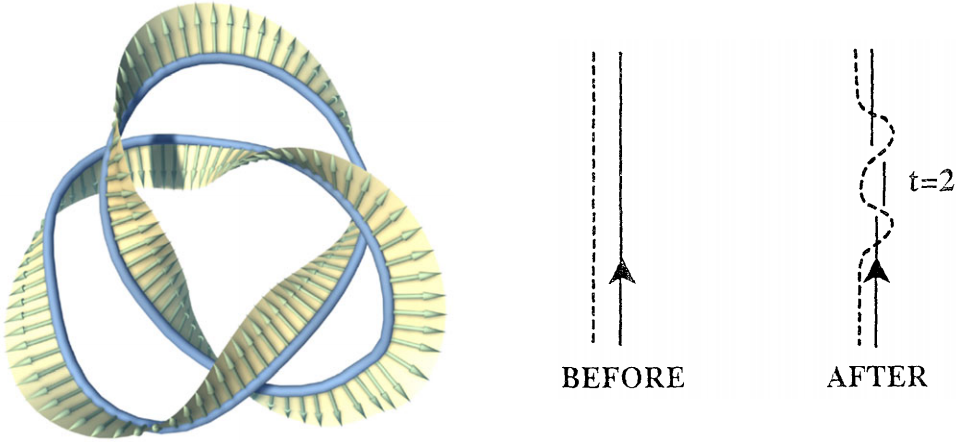
\includegraphics[width=0.85\textwidth]{figures/fig3_trefoil_framing.png}
  \caption{左：三叶结标架的一个选择，就是一个与它正交、把它「框住」的向量场 \cite{elhamdadi2020}。右：标架变换可以看成 $\gamma'$ 相对 $\gamma$ 的一次扭转 \cite{witten1989}。（原文 Figure 3，原文 p.23）}
  \label{fig:framing}
\end{figure}

% 原文标题：Examples and caveats.
\paragraph{例子与告诫} 收尾时，把展开理论过程中漏掉的评论、例子与警告一并补上。先看几个显式配分函数。对 $M=S^2\times S^1$，任意规范群 $G$ 都有 $\mathcal{Z}=1$。对 $M=S^3$，规范群 $G=\mathrm{U}(1)$ 时可用结果 \eqref{eq:3.30}：取空链环，相位为零，故 $\mathcal{Z}=1$。对 $M=S^3$ 与非阿贝尔 $G$，唯一的平坦联络是平凡联络 $A^{(\alpha)}=0$。有人或许想套用 \eqref{eq:3.27}，但（下面会讨论）它在这里其实失效。$G=\mathrm{SU}(2)$ 的实际结果及其大 $k$ 标度行为是

\begin{equation}\tag{3.32}\label{eq:3.32}
  \mathcal{Z} = \sqrt{\frac{2}{k+2}}\,\sin\left(\frac{\pi}{k+2}\right) \sim k^{-3/2}.
\end{equation}

注意 $c_2(\mathrm{SU}(2))=4$，所以这里出现的因子 $k+2$ 其实就是单圈下「重整化」过的陈--西蒙斯能级 $k+\frac{c_2(G)}{2}$。另外，有件颇有意思的小事：规范群 $G=\mathrm{SU}(5)$ 有 $d=\dim G=24$，把它代入 \eqref{eq:3.28}，$\mathcal{Z}$ 对 $M$ 的标架的依赖就彻底消失了。

最后，我们指出 \S\ref{sec:3.2} 里一条重要的告诫：算子 $\Delta$ 与 $L_-$ 的行列式必须非零，\eqref{eq:3.17} 的一切推论才说得通。事实上，这些算子非奇异，当且仅当 $A^{(\alpha)}$ 平凡化所有德拉姆上同调群 $H^n_{\mathrm{dR}}(M,E)$。这些对象来自一个观察：在平坦丛上，$[D_\mu,D_\nu]=F_{\mu\nu}=0$ 蕴含 $D\circ D=0$。于是协变导数是由平坦联络 $A^{(\alpha)}$ 扭出的上边缘算子，上同调定义为 $H^n_{\mathrm{dR}}(M,E)=\bigl(\ker D|_{\Omega^n(M,E)}\bigr)\big/\bigl(\operatorname{im}D|_{\Omega^{n-1}(M,E)}\bigr)$。让我们的结果失效，最省事的办法

% ==== 原文 p.24 ====
是找一个 $H^0(M,E)\neq0$ 的情形。一旦如此，算子 $\Delta$ 与 $L_-$ 就有零本征值，辅助场 $\phi$、$\bar c$、$c$ 就有零模，定规范随之变复杂。$M=S^3$ 时正是如此，那里唯一的平坦联络是平凡联络。具体说，$H^0(M,E)=\ker\dd|_{C^\infty(M,E)}=E\neq0$，即常值映射 $M\to E$ 的集合。所以，虽有「平凡」之名，平凡联络却惹来大麻烦。最后我们注意到：若 $H^1_{\mathrm{dR}}(M,E)\neq0$，平坦联络便不孤立、数目也不再有限，而是落在一个更大的平坦联络模空间里。

% =============================================================================
% 交付汇报（片段 s03b）
% * 覆盖原文 p.19–p.24（至 "…larger moduli space of flat connections." 止），
%   编号公式 (3.25)–(3.32) 共 8 个（\tag 锁定、顺序照原文），图 3，脚注 7。
% * 译注 8 条：易错点 4 条（(3.25) 的 1/4π 与 ω 取值；(3.26) 相位代数与波浪箭头；
%   (3.27)–(3.28) 的 d=dim G 与 24；(3.30)–(3.31) 的 4π 归一化与 n_a^2），
%   含糊点 3 条（APS [15–17]、[18][19]+[9]、Schwarz [14] 的 Ray–Singer 挠率），
%   原文疑误 1 条（p.20 的 η_g=η_g）。
% * SPEC §10 裁定：
%   第 10 条成立：p.20 图像确作 "η_g = η_g"，照录 + 批注。
%   第 11 条不成立：p.21 图像 (3.26) 中第二个等号后是波浪箭头（\leadsto），
%     提取文本误作「/」；相位符号与 (3.27) 一致，无矛盾，故按图像录为箭头、
%     不写「原文疑误」批注。
%   第 12 条已核，无误：d=dim G=24 时 e^{2πis}=1，标架依赖消失。
% * 另见存疑：p.23 "all of the the de Rham cohomology groups" 重复一个 the
%   （中文不可见，未加注，报 Lead）；(3.30) 第二行与第一行系数之差 4π 已在译注说明。
% =============================================================================
% >>>>>>>>>>>>>>>> end sections/s03b-framing2.tex <<<<<<<<<<<<<<<<

% >>>>>>>>>>>>>>>> sections/s04a-hilbert.tex <<<<<<<<<<<<<<<<
% ==== 原文 p.24 ====
\section{希尔伯特空间结构}\label{sec:4}

% [Tutor Note: 本节重点] 物理图像/数学工具/主要结论
\begin{keytakeaways}
\begin{itemize}[leftmargin=1.4em,itemsep=2pt,topsep=2pt]
  \item \textbf{物理图像：}把 3 维流形 $M$ 沿曲面 $\Sigma$ 切开，理论就化成 $\Sigma\times\R$ 上的正则量子化：$\R$ 是时间，$\Sigma$ 是“空间”。$\Sigma$ 的拓扑只允许有限多个非平凡威尔逊圈，相空间因而缩成紧致、有限体积的平坦联络模空间，量子化得到的希尔伯特空间是有限维的。
  \item \textbf{数学工具：}平坦联络模空间 $\mathcal{M}$（Atiyah--Bott 的维数与奇点分析）、几何量子化与全纯量子化、前量子线丛与陈联络、行列式线丛（Quillen 的 $\bar\partial$ 行列式）、小平嵌入定理、模函子（Segal）。
  \item \textbf{主要结论：}$\mathcal{H}_\Sigma$ 是紧凯勒模空间 $\mathcal{M}_J$ 上某条正线丛的全纯截面空间，故有限维；$k=1$、$G=\mathrm{SU}(N)$ 时这条线丛正是 $\bar\partial$ 的行列式线丛，一般能级与一般群则取它的张量幂；$\mathcal{H}_\Sigma$ 不依赖复结构 $J$，$\Sigma\mapsto\mathcal{H}_\Sigma$ 构成一个模函子。
\end{itemize}
\end{keytakeaways}

% [Tutor Note: 易错点] p.24--p.28 上同一字母有多种写法：3 维流形 $M$、平坦联络模空间 $\mathcal{M}$、固定复结构的 $\mathcal{M}_J$、黎曼面模空间 $\mathcal{M}_\Sigma$；相空间另记 $\mathcal{P}$，希尔伯特空间记 $\mathcal{H}_\Sigma$。
\begin{yizhu}[易错点]
从本节起，同一字母有多种写法，务必按上下文分清：3 维流形用普通体 $M$（原文 “the 3-manifold $M$”）；平坦联络模空间用花体 $\mathcal{M}$（原文 “the resulting phase space $\mathcal{M}$”）；选定复结构后写 $\mathcal{M}_J$；$\Sigma$ 上复结构本身的模空间写 $\mathcal{M}_\Sigma$。相空间记 $\mathcal{P}$，希尔伯特空间记 $\mathcal{H}_\Sigma^{(J)}$，二者都不是 $M$。原文 $M$ 与 $\mathcal{M}$ 在版面上只差一个花体，读 p.24--p.28 时须逐处确认。
\end{yizhu}

\paragraph{开战}
% 原文标题：Into the fray.
这一节，我们放下路径积分，去承担一个雄心勃勃的目标：精确求解陈--西蒙斯理论。所谓“求解”，就是尽可能精确地描述该理论的希尔伯特空间，以及物理可观测量的结构。策略沿用 Witten 的洞见 \cite{witten1989}：（1）把理论所在的 3 维流形 $M$ 切成更简单的碎片；（2）用正则量子化在每个碎片上求解；（3）把威尔逊圈加进来；（4）再把碎片粘回去。本节余下篇幅用来铺陈这个计划的若干细节。后面的讨论相当抽象，请随时把 \S\ref{sec:2.3} 的想法放在手边。我们仍会写得相当印象派，也会略去一些技术细节。

\begin{figure}[htbp]
  \centering
  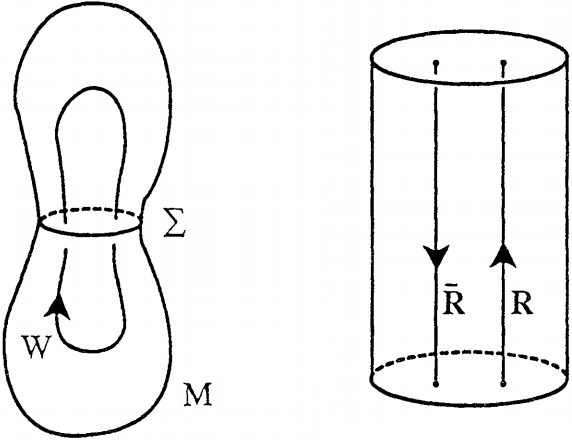
\includegraphics[width=0.5\textwidth]{figures/fig4_wilson_loop.png}
  \caption{左：一个含威尔逊圈 $W$ 的 3 维流形 $M$，沿黎曼面 $\Sigma$ 切开。右：切口处的领状邻域。曲面 $\Sigma$ 上有两个代表电荷的标记点，$W$ 的出射段与入射段在这两点插入表示 $R$ 与 $\bar R$ \cite{witten1989}。（原文 Figure 4，原文 p.24）}
  \label{fig:cut}
\end{figure}

\paragraph{提要}
% 原文标题：Synopsis.
每个可定向 3 维流形都可以沿一张 2 维曲面 $\Sigma$ 切成两块不相交的碎片。$\Sigma$ 作为可定向 2 维流形，可以赋予复结构，于是成为一张黎曼面。（$\Sigma$ 没有\textit{典范}复结构，这一点后面会变得重要。）切口附近，$M$ 的拓扑是 $\Sigma\times\R$；画面就像切一块瑞士奶酪。于是我们考虑这种拓扑的流形上的 CS 理论；把 $\R$ 当作时间方向，就得到与 $\Sigma$ 相配的希尔伯特空间 $\mathcal{H}_\Sigma$。一路上会遇到一个意外：高斯定律约束如今是非线性的。
% ==== 原文 p.25 ====
它使 $\mathcal{H}_\Sigma$ 成为有限维的。从精神上说，原因在于：$\mathcal{H}_\Sigma$ 来自理论的经典相空间，而这个相空间只由有限多个相位（phase）参数化，这些相位来自 $\Sigma$ 的拓扑所允许的非平凡威尔逊圈。我们也可以像以前一样，在 $M$ 里放纽结来加入源。其中有些纽结会穿过 $\Sigma$，于是出现图 \ref{fig:cut} 的画面。这时 $\Sigma$ 上带着若干“标记”点 $p_i$——纽结在此穿过——每个标记点附着相应威尔逊圈所给的表示 $R_i$。由这些数据构造 $\mathcal{H}_\Sigma$ 更为复杂，我们只勾勒做法。

% [Tutor Note: 物理图像] “有限多个相位”有来历：§2.3 的环面上相空间就是 $T^2$，两个威尔逊圈的和乐各是一个 $U(1)$ 纯相位；亏格 $g$ 时 $\pi_1(\Sigma)$ 有 $2g$ 个生成元，给出 $2g$ 个相位。
\begin{yizhu}[物理图像]
“由有限多个相位参数化”一句有来历。\S\ref{sec:2.3} 里环面上的经典相空间就是 $T^2$：$\pi_1(T^2)=\Z\oplus\Z$ 的两个生成元各给一个威尔逊圈，其和乐都是 $\mathrm{U}(1))$ 的纯相位，两个相位就是相空间的坐标。亏格 $g$ 的曲面同理给出 $2g$ 个相位。非阿贝尔情形还要加入色的数据，相空间随之升格为模空间。
\end{yizhu}

\subsection{全纯量子化}\label{sec:4.1}

\paragraph{正则形式}
% 原文标题：The canonical formalism.
我们从 $M=\Sigma\times\R$ 上的 CS 作用量 \eqref{eq:3.3} 出发。取规范 $A_0=0$，所得结果与 \S\ref{sec:2.3} 几乎一样，唯一区别是多了群论指标。作用量化为
\begin{equation}\tag{4.1}\label{eq:4.1}
  \SCS = \frac{k}{4\pi}\int_{\R}\dd t\int_{\Sigma}\dd^2 x\,\varepsilon^{ij}\Tr\bigl(A_i\dot A_j\bigr).
\end{equation}

% [Tutor Note: 易错点] (4.1) 与 (2.22) 逐字同形，只多一个 $\Tr$；系数 $k/4\pi$ 不含额外的 $1/2$。(2.20) 把同一作用量写成 $\frac{k}{2\pi}(\frac12\varepsilon^{ij}A_i\dot A_j+A_0B)$，那个 $1/2$ 已被 $k/2\pi$ 吸收。
\begin{yizhu}[易错点]
\eqref{eq:4.1} 是 \eqref{eq:2.22} 的非阿贝尔版：两式逐字同形，只多了一个 $\Tr$，系数就是 $k/4\pi$，\emph{不要}再补 $1/2$。核对看 \eqref{eq:2.20}：作者把同一作用量改写成 $\frac{k}{2\pi}\int(\frac12\varepsilon^{ij}A_i\dot A_j+A_0B)$，$1/2$ 是被 $k/4\pi\to k/2\pi$ 吸收掉的；在 \eqref{eq:4.1} 里再添 $1/2$，结果就差一倍。符号上取 $\varepsilon^{12}=+1$，则 $\varepsilon^{ij}A_i\dot A_j=A_1\dot A_2-A_2\dot A_1$，与 \eqref{eq:2.5} 的 $B=\varepsilon^{ij}\partial_iA_j$ 用同一约定。非阿贝尔情形下 $\Tr(A_i\dot A_j)$ 的两个因子不能交换，$\dot A_j$ 指 $\partial_tA_j$。
\end{yizhu}

和以前一样，哈密顿量为零，“坐标”是 $A_i$，“动量”是 $\varepsilon^{ij}A_j$。可见和以前一样，规范场与自己正则共轭。$A_\mu=(0,A_i^aT^a)$ 的空间分量满足正则泊松括号
\begin{equation}\tag{4.2}\label{eq:4.2}
  \bigl\{A_i^a(\mathbf{x}), A_j^b(\mathbf{y})\bigr\}
  = \frac{2\pi}{k}\,\varepsilon_{ij}\delta^{ab}\delta^{(2)}(\mathbf{x}-\mathbf{y}).
\end{equation}

% [Tutor Note: 易错点] (4.2) 与 (2.23) 有三处差别：多色指标 $a,b$ 与 $\delta^{ab}$（隐含正交基）；只给泊松括号，量子化后要补 $i$；$\varepsilon_{ij}$ 是下标，而 (4.1)(4.3) 用上标 $\varepsilon^{ij}$。
\begin{yizhu}[易错点]
\eqref{eq:4.2} 与 \eqref{eq:2.23} 的泊松括号相比有三处要看住。其一，右侧多了色结构 $\delta^{ab}$：这只在 $\Tr(T^aT^b)\propto\delta^{ab}$ 的正交基下成立，一般基底下应换成基灵型的逆 $K^{ab}$。其二，\eqref{eq:2.23} 把泊松括号与对易子并列，后者带 $i$；\eqref{eq:4.2} 只给经典括号，正则量子化后还得自己补 $i$。其三，这里的 $\varepsilon_{ij}$ 是下标，而 \eqref{eq:4.1}、\eqref{eq:4.3} 写的是上标 $\varepsilon^{ij}$；欧氏二维度规升降号不改分量，但抄录时不可随手改。
\end{yizhu}

这个关系定义了一个经典相空间，但它太大了：经典 CS 理论还受非阿贝尔高斯定律约束，此约束把我们限制在平坦联络上：
\begin{equation}\tag{4.3}\label{eq:4.3}
  \varepsilon^{ij}F_{ij}^a = 0 \quad\Longleftrightarrow\quad F = 0.
\end{equation}

% [Tutor Note: 易错点] $\varepsilon^{ij}F^a_{ij}=2F^a_{12}$：约束本身仍等价于 $F=0$，但因子 2 必须与 (2.21) 的 $B=F_{12}$ 及 (4.5) 的源项 $\frac{k}{4\pi}\varepsilon^{ij}F^a_{ij}$ 配套，丢了它就差一倍。
\begin{yizhu}[易错点]
$\varepsilon^{ij}F^a_{ij}=\varepsilon^{12}F^a_{12}+\varepsilon^{21}F^a_{21}=2F^a_{12}$，所以 \eqref{eq:4.3} 的左边是 $F^a_{12}$ 的两倍。因子 2 不改变“$=0$”这个结论（$F_{ij}$ 反对称，二维只有一个独立分量），但它必须与另外两式配套：\eqref{eq:2.21} 写的是 $\frac{k}{2\pi}B=\frac{k}{2\pi}F_{12}=0$；\eqref{eq:4.5} 写的是 $\frac{k}{4\pi}\varepsilon^{ij}F^a_{ij}=\sum_s\delta^{(2)}(x-x_s)T^a_s$。若把 \eqref{eq:4.3} 左边读成 $F^a_{12}$，\eqref{eq:4.5} 的源项就会差一倍。
\end{yizhu}

\paragraph{作战方案}
% 原文标题：Plan of attack.
由于 $F=\dd A+A\wedge A$ 对规范场是二次的，约束 \eqref{eq:4.3} 把非线性重新塞回 \eqref{eq:4.1}--\eqref{eq:4.2} 所定义的、本来极其自由的理论。要照 \S\ref{sec:2.3} 铺开的“先量子化、再约束”流程走，几乎不可能：在波泛函层面实施 \eqref{eq:4.3}（如 \eqref{eq:2.26} 那样），会得到一个严重非线性的偏微分方程，从而限死物理上允许的态。我们反过来做：“先约束、再量子化”，在经典层面就实施 \eqref{eq:4.3}。所得的相空间 $\mathcal{M}$ 称为平坦联络的\textit{模空间}；其元素是规范丛 $E\to\Sigma$ 上平坦主 $G$-联络 $A$ 的规范等价类。Atiyah 与 Bott \cite{atiyahbott1982} 研究过它，并证明：$\mathcal{M}$ 是紧致的、流形般的对象，只有温和奇点；它从 \eqref{eq:4.2} 的无约束相空间继承辛结构；实维数为 $d(2g-2)$，其中 $d=\dim G$，$g$ 是 $\Sigma$ 的亏格。又因 $\mathcal{M}$ 紧致，它的（辛）体积有限。依照海森堡不确定性原理，量子化通常在相空间的每单位体积产生一个量子自由度。于是我们看到，$\mathcal{M}$ 的量子化应当给出有限维的希尔伯特空间。

% [Tutor Note: 原文疑误] 原文 p.25 “It would be virtually impossible to follow the the “quantize, then constrain” procedure” 连写两个 the，属排印重复；译文按单次处理。
\begin{yizhu}[原文疑误]
原文此句作 “It would be virtually impossible to follow the the ‘quantize, then constrain’ procedure laid out in §2.3”，连写两个 the，属排印重复（原文 p.25）。译文按单次处理；若对照英文阅读，此处不必再找第二个定冠词。
\end{yizhu}

% [Tutor Note: 含糊点] $d(2g-2)$ 的来源是形变复形的上同调维数：不可约时 $H^0=0$，$\dim H^1=d(g-1)$，实维数加倍。Atiyah–Bott [21] 用指标定理算出；仅适用于 $g\ge2$ 的不可约部分。
\begin{yizhu}[含糊点]
维数 $d(2g-2)=2d(g-1)$ 是实维数，作者没有推导。它来自平坦联络形变复形的上同调：不可约联络满足 $H^0=0$，欧拉示性数 $d(1-g)$ 给出 $\dim H^1=d(g-1)$，实维数加倍即得。Atiyah--Bott \cite{atiyahbott1982} 用杨--米尔斯方程解空间的指标定理算出它，并说明奇点来自可约联络。该式只对 $g\ge2$ 的不可约部分成立：$g=0$ 时模空间退化为单点，$g=1$ 时维数为 $2\operatorname{rank}G$（$G=\mathrm{U}(1))$ 时就是 $T^2$），公式分别给出负值与零。
\end{yizhu}

% ==== 原文 p.26 ====
\paragraph{几何量子化}
% 原文标题：Geometric quantization.
在量子力学中 \cite{woodhouse}，我们通常从相空间 $\mathcal{P}$ 出发，它由坐标 $q^i$ 与动量 $p^i$ 参数化；然后把希尔伯特空间 $\mathcal{H}$ 定义为 $q^i$ 的复值平方可积函数空间。这个构造有两个显著特征：它要求把相空间变量拆成坐标与动量；并且它“挑出”其中一半坐标。（这种选择称为\textit{极化}。）我们可以用几何语言重写这个构造：在 $\mathcal{P}$ 的每一点附上一个复平面的副本，再把波函数 $\psi$ 定义为所得 $\C$-丛的任一截面（这个丛还没指定，马上会说），且满足两个条件。第一，$\psi$ 平方可积；第二，它只依赖 $q^i$、不依赖 $p^i$，即 $\partial\psi/\partial p^i=0$。坦白说，这个观点有点别扭——但别扭是故意的，因为接下来我们会看到它变得何等有力。

\paragraph{凯勒量子化}
% 原文标题：Kähler quantization.
\textit{凯勒流形}同时是辛流形、复流形与黎曼流形，三种结构彼此相容。\footnote{在某种意义上，它是一个相空间（因为它是辛的），却像一个弯曲的希尔伯特空间（因为它是复的，且带有切空间内积）。说得更直白些：凯勒流形就是一个花哨的甜甜圈。}
若相空间 $\mathcal{P}$ 恰好是凯勒的，我们就可以用新变量 $z^i=q^i+ip^i$ 与 $\bar z^i=q^i-ip^i$ 来参数化它。上面的 $\C$-丛变成 $\mathcal{P}$ 上的复线丛 $L$；我们只接受那些依赖 $z^i$、不依赖 $\bar z^i$ 的截面 $\psi\colon\mathcal{P}\to L$ 充当波函数。于是希尔伯特空间就定义为 $L$ 的\textit{全纯截面}空间。这类截面满足 $\partial\psi/\partial\bar z^i=0$，因此 $L$ 上的 $\bar\partial$ 算子湮灭它们。至于“平方可积性”，那需要一个内积。给 $L$ 配一个厄米度规就能算内积，例如 $\langle\psi|\psi\rangle$。厄米度规在 $L$ 上确定唯一的联络（其实就是列维--奇维塔联络！），称为\textit{陈联络} $\mathcal{A}$；它与 $\mathcal{P}$ 上的凯勒结构以两种方式相容。第一，由 $\mathcal{A}$ 构造的协变导数 $\mathcal{D}$ 与 $\bar\partial$ 算子相同，故物理波函数是协变常数的：$\mathcal{D}\psi=0$。第二，$\mathcal{A}$ 的曲率 $\Omega$ 满足 $\Omega=-i\omega$，其中 $\omega$ 就是（！）$\mathcal{P}$ 上的辛形式。接下来是一个奇迹：线丛的第一陈类 $c_1(L)=[\frac{i}{2\pi}\Omega]$ 是拓扑不变量，唯一地刻画 $L$。于是只要 $\mathcal{P}$ 的辛结构给定，所需的线丛就唯一确定了。

% [Tutor Note: 易错点] $\Omega=-i\omega$、$c_1(L)=[\frac{i}{2\pi}\Omega]$、$c_1(L)=[\frac{\omega}{2\pi}]$ 三式一致：$\frac{i}{2\pi}(-i\omega)=\frac{\omega}{2\pi}$。把 $-i$ 记成 $+i$ 会使 $c_1$ 变号、$\Omega$ 失去正定性。
\begin{yizhu}[易错点]
$\Omega=-i\omega$ 与两个陈类表达式是同一件事：代入即得 $\frac{i}{2\pi}\Omega=\frac{i}{2\pi}(-i\omega)=\frac{\omega}{2\pi}$。若把 $\Omega=-i\omega$ 的 $-i$ 记成 $+i$，$c_1(L)$ 整体变号，$\Omega$ 也不再正定。这里 $\omega$ 取实辛形式，$\Omega$ 是 $(1,1)$-形式；符号约定与陈类定义 $c_1=\frac{i}{2\pi}\Tr F$ 绑死。
\end{yizhu}

于是总结如下：设 $\mathcal{P}$ 是辛形式为 $\omega$ 的凯勒流形，取第一陈类为 $c_1(L)=[\frac{\omega}{2\pi}]$ 的线丛 $L$，今后称之为 $\mathcal{P}$ 的\textit{前量子线丛}。给 $L$ 配上陈联络；它确定 $L$ 上的厄米内积，曲率为 $\Omega=-i\omega$。那么与 $\mathcal{P}$ 相配的希尔伯特空间 $\mathcal{H}$ 就是 $L$ 的全纯截面空间；若 $\mathcal{P}$ 紧致，则 $\mathcal{H}$ 有限维。

\paragraph{希尔伯特空间}
% 原文标题：The Hilbert space.
回到本例：相空间 $\mathcal{P}=\mathcal{M}$ 并不带自然的复结构或凯勒结构。然而可以证明：一旦在曲面 $\Sigma$ 上选定复结构 $J$，模空间 $\mathcal{M}=\mathcal{M}_J$ 也就继承了复结构与凯勒结构。粗略地说，做法是先把规范群 $G$ 复化为 $G_\C$，然后（呼应上面的全纯量子化）在 $G_\C$ 中选一片“切片”，迫使复化规范丛上的联络全纯地变化。

% [Tutor Note: 含糊点] “it can be shown ... $\mathcal{M}_J$ inherits complex and Kähler structures” 省掉两步：复化 $G_\C$ 后平坦联络等价于全纯结构（Narasimhan–Seshadri / Kobayashi–Hitchin 对应）；切片把复化空间切回实子流形，Atiyah–Bott 的辛形式配上复结构给出凯勒结构。
\begin{yizhu}[含糊点]
此处 “it can be shown” 吞掉了两步论证。第一步，$G$ 复化为 $G_\C$ 后，“$G_\C$-联络的复规范等价类”与“$E$ 上的全纯结构 $\bar\partial_A$”是同一件事：次数为零的稳定全纯丛对应不可约平坦酉联络，即 Narasimhan--Seshadri 定理，其高秩推广为 Kobayashi--Hitchin 对应（$G=\mathrm{SU}(N)$ 时又称 Donaldson--Uhlenbeck--Yau 定理）。第二步，“取切片”把复化后的联络空间切回实子流形；$\mathcal{M}_J$ 的凯勒结构由 Atiyah--Bott \cite{atiyahbott1982} 的辛形式配上这个复结构给出。原文对这两步都未标文献。
\end{yizhu}

% ==== 原文 p.27 ====
一旦做出这个选择，$\mathcal{M}_J$ 从 \eqref{eq:4.2} 继承的辛形式 $\omega$ 就确定了第一陈类为 $c_1(L)=[\frac{\omega}{2\pi}]$ 的唯一线丛 $L$。接着用 $L$ 上的陈联络构造协变导数 $\mathcal{D}$，它与 $L$ 上的 $\bar\partial$ 算子一致；正是后者定义了全纯截面，而这些截面终于把希尔伯特空间 $\mathcal{H}_\Sigma^{(J)}$ 赋予 $\Sigma$。这番讨论坦白说相当抽象，但我们会在 \S\ref{sec:4.3} 看到一些例子。

当 $G=\mathrm{SU}(N)$、$k=1$ 时，$L$ 有一个稍具体的描述：基本想法是用 $\Sigma$ 上 $\bar\partial$ 算子产生的一族算子来构造 $L$。回忆取 $A_0=0$ 规范后，规范丛 $E\to M$ 可以看作 $\Sigma$ 上的丛。一旦固定 $\Sigma$ 上的复结构、把规范群复化为 $G_\C$、再选定 $G_\C$ 的一个表示（比如基础表示），$E$ 就获得 $\Sigma$ 上全纯向量丛的结构。$\mathcal{M}_J$ 的每一点是 $E$ 上的平坦联络；由该联络构造的协变导数保留了 $E$ 上复结构的部分信息。事实上，我们可以用它去“扭” $\Sigma$ 上本来就有的 $\bar\partial$ 算子——那是 $\Sigma$ 自身复结构给的。这样，$\mathcal{M}_J$ 就参数化 $E$ 上一族被扭的 $\bar\partial$ 算子。

\paragraph{行列式线丛}
% 原文标题：The determinant bundle.
现在有一种漂亮办法，给每个被扭的 $\bar\partial$ 算子（也就是 $\mathcal{M}_J$ 的每一点）配一条复线，从而得到前量子线丛。该构造由 Quillen \cite{quillen1986} 引入，做法基本上是“取 $\bar\partial$ 的行列式”。人们把行列式看作“取 $E$ 的最高外幂”这一操作的替身；最高外幂给出一个一维空间，当作一条线。更确切地说，给每个 $\bar\partial$ 算子配上一条线
\begin{equation}\tag{4.4}\label{eq:4.4}
  \mathcal{L}_{\bar\partial}
  = \bigwedge^{n}(\ker\bar\partial)^{*}\otimes\bigwedge^{n}(\operatorname{coker}\bar\partial).
\end{equation}
最后，把这些线粘起来，就定义了 $\mathcal{M}_J$ 上的\textit{行列式线丛} $L$。

% [Tutor Note: 易错点] (4.4) 的 $n$ 是 $\ker\bar\partial$ 的维数，不是 $E$ 的秩、也不是固定的外幂阶数；两侧同写一个 $n$ 隐含指标为零。取对偶的是 $\ker$ 一侧，换到 $\operatorname{coker}$ 一侧则 $c_1$ 变号。
\begin{yizhu}[易错点]
\eqref{eq:4.4} 的 $n$ 是 $\ker\bar\partial$ 的维数（两侧写同一个 $n$，隐含 $\dim\ker=\dim\operatorname{coker}$，即指标为零），不是 $E$ 的秩，也不是一个固定的外幂阶数。按黎曼--罗赫，$\operatorname{ind}\bar\partial_E=\deg E+\operatorname{rank}E\,(1-g)$；平坦联络给出 $\deg E=0$，但 $\operatorname{rank}E\,(1-g)$ 一般不为零，此时两侧维数并不相等，Quillen 的标准约定是取极大外幂。另外，取对偶的是 $\ker$ 这一侧：改到 $\operatorname{coker}$ 一侧，得到的就对偶线丛，$c_1$ 与曲率整体变号。
\end{yizhu}

% [Tutor Note: 含糊点] “狄拉克行列式给出厄米度规” 背后是 \$\\ 的模长按 $\exp(-\frac12\zeta'(0))$ 定义；Quillen [23] 把它与 $L^2$ 度规合成行列式线丛上的厄米度规，并证明曲率为 $-i\omega$。
\begin{yizhu}[含糊点]
“狄拉克行列式给出厄米度规”背后是 \$\\ 的行列式不是有限维行列式，其模长按 $\exp(-\frac12\zeta'(0))$ 定义，$\zeta$ 取自 $\bar\partial^*\bar\partial$ 的非零谱。Quillen \cite{quillen1986} 用它配上 $L^2$ 度规，在行列式线丛上定义厄米度规（今称 Quillen 度规），并证明该度规的曲率恰为 $-i\omega$、第一陈类为 $[\frac{\omega}{2\pi}]$。这正是“行列式线丛就是前量子线丛”的实质。
\end{yizhu}

可以验证：当 $k=1$ 时，这就是正确的线丛。狄拉克行列式在 $L$ 上给出厄米度规并确定陈联络，从而可以算出它的曲率与第一陈类。这件事由 Quillen 完成；他证明两者都符合 $c_1(L)=[\frac{\omega}{2\pi}]$ 与 $\Omega=-i\omega$，与辛形式 \eqref{eq:4.2} 一致。当 $k\neq1$ 时，行列式线丛 $L$ 把辛形式算错了一个因子 $k$；一般说来，能级 $k$ 上正确的线丛是 $L^{\otimes k}$。而当 $G\neq\mathrm{SU}(N)$ 时，出现的则是 $L^{\otimes k}$ 的某个（可能很大的）张量幂，这要归功于小平嵌入定理。

% [Tutor Note: 含糊点] 小平嵌入定理：紧复流形上正线丛（$c_1>0$ 的 ample 丛）的足够高张量幂给出到射影空间的嵌入。作者只说“某个（可能很大的）张量幂”，既不给幂次也不给构造，原文亦未标文献编号。
\begin{yizhu}[含糊点]
小平嵌入定理（Kodaira）说：紧复流形上若存在正线丛（$c_1>0$ 的 ample 线丛），则它的足够高张量幂给出到射影空间的嵌入。作者借它论证：$G\neq\mathrm{SU}(N)$ 时，前量子线丛未必是行列式线丛本身，而是其某个高次张量幂。这一步只保证存在性，幂次多大、线丛具体如何构造，原文都未说明，也未标出该定理的文献编号（标准出处为小平 1954）。
\end{yizhu}

\paragraph{模函子}
% 原文标题：The modular functor.
现在回到一个已反复出现的主题：$\Sigma$ 上没有典范的复结构。事实上，这类复结构 $J$ 在它们自己的黎曼面模空间里变动，我们记作 $\mathcal{M}_\Sigma$。从物理上讲，上面构造的希尔伯特空间 $\mathcal{H}_\Sigma^{(J)}$ 不能依赖复结构 $J$。理由在于：$\mathcal{H}_\Sigma^{(J)}$ 是一个问题的解，而该问题的提法只依赖可定向曲面 $\Sigma$，不依赖它的复结构。一个理论没有资格“知道” $J$，改变 $J$ 就不该影响它的希尔伯特空间。

% ==== 原文 p.28 ====
于是我们可以把各个 $\mathcal{H}_\Sigma^{(J)}$ 看作某个向量丛在模空间 $\mathcal{M}_\Sigma$ 上的纤维；这个丛的底点就是 $\Sigma$ 上的复结构 $J$。各纤维既然全同，丛就应当容许一个平坦联络，把纤维典范地等同起来。于是可以用 $\mathcal{H}_\Sigma$ 代替 $\mathcal{H}_\Sigma^{(J)}$，并得到一个映射：把曲面 $\Sigma$ 送到它的 CS 希尔伯特空间 $\mathcal{H}_\Sigma$。模空间上的这类平坦丛由 Segal \cite{segal} 研究过；他把映射 $\Sigma\mapsto\mathcal{H}_\Sigma$ 称为\textit{模函子}。

% ==== 片段汇报（s04a-hilbert） ====
% 覆盖：原文 p.24（§4 标题、Into the fray、图 4、Synopsis）—p.28（模函子段末，4.2 之前）。
% 编号公式：4 个，(4.1)--(4.4)，\tag 锁定。
% 图：图 4（figures/fig4_wilson_loop.png，width=0.5\textwidth，label=fig:cut），图注全译。
% 脚注：第 8 条（p.26）全译，位于“三种结构彼此相容”之后。
% 译注：12 条（易错点 6、含糊点 4、原文疑误 1、物理图像 1）。
% 记号裁定：图注 “R and R̄” 为 $\bar R$（PDF 中 R 上横线，非 $R^*$）。
% 维数裁定：$d(2g-2)$ 只适用于 $g\ge2$ 不可约情形；$g=0$ 单点、$g=1$ 为 $2\operatorname{rank}G$。
% 疑误：(a) p.25 “the the” 排印重复，照译并批注；(b) (4.2) 的 $\varepsilon_{ij}$ 与 (4.1)(4.3) 的 $\varepsilon^{ij}$ 上下标不一致，照录并批注。
% 待确认：无。
% >>>>>>>>>>>>>>>> end sections/s04a-hilbert.tex <<<<<<<<<<<<<<<<

% >>>>>>>>>>>>>>>> sections/s04b-hilbert2.tex <<<<<<<<<<<<<<<<
% ==== 原文 p.28 ====
\subsection{带源的量子化}\label{sec:4.2}
% 原文标题：4.2 Quantization with Sources

\paragraph{插入威尔逊圈}
我们现已准备好做一件真正有物理意义的事：描述有物质存在时 CS 理论的希尔伯特空间结构。等价地，正如 \S\ref{sec:2.2} 中所见，只要考虑存在威尔逊圈的理论，我们就能把 $\SCS$ 与源耦合起来。图 \ref{fig:cut} 示意了这一点。它提示：一个威尔逊圈在 $\Sigma$ 上留下的印记，是一组静态的非阿贝尔电荷。在 $A_0=0$ 规范下，设 $\Sigma$ 上的点 $p_1,\dots,p_r$ 处有 $r$ 个这样的电荷，则 CS 理论的高斯定律成为
\begin{equation}\tag{4.5}\label{eq:4.5}
  \frac{k}{4\pi}\varepsilon^{ij}F^{a}_{ij} = \sum_{s=1}^{r}\delta^{(2)}(x-p_s)T^{a}_{s}.
\end{equation}
这里 $T^{a}_{s}\in\mathfrak{g}$ 是分配给每个电荷的李代数生成元。在量子理论中，这些生成元应按相应的表示 $R_s$ 来理解。

% [Tutor Note: 易错点] (4.5) 左端的 k/4π 来自 S_CS 对 A_0 的变分，与 (4.2) 的 2π/k 角色不同、不可互换；ε^{ij} 与 ε_{ij} 的上下标、δ^(2) 的密度性质都须留意。
\begin{yizhu}[易错点]
(4.5) 左端的 $k/4\pi$ 来自 $\SCS$ 对 $A_0$ 的变分，不要与 \eqref{eq:4.2} 的 $2\pi/k$ 混用：后者是辛形式（泊松括号）的归一化，前者是约束方程的系数，两者出自同一个 $\SCS$ 却各司其职。又因 $\varepsilon^{ij}F_{ij}=2\varepsilon^{ij}\partial_iA_j$ 带因子 $2$，两个系数相乘只给出 $1/2$ 而不是 $1$，不能靠「互逆」来记忆。指标上，左端用 $\varepsilon^{ij}$，\eqref{eq:4.2} 用 $\varepsilon_{ij}$：在平坦 $\R^2$ 上二者数值相同，搬到弯曲 $\Sigma$ 上须换成面积形式，$\delta^{(2)}$ 也应按密度理解。
\end{yizhu}

% [Tutor Note: 易错点] T^a_s 在 (4.5) 里是李代数元，在量子理论里是表示 R_s 中的算子；反厄米性使 iT^a_s 才是可观测量，这是后文「去量子化」的依据。
\begin{yizhu}[易错点]
$T^{a}_{s}$ 在两处含义不同。在 (4.5) 这个经典约束里，它是 $\mathfrak{g}$ 中为每个电荷选定的生成元；进入量子理论后，它必须读作表示 $R_s$ 中的算子 $T^{a}(R_s)$，每个标记点带自己的表示。因此 (4.5) 的右端是算符值分布，不同 $s$ 的 $T^{a}_{s}$ 作用在各自的表示上，严格说要先写进张量积 $R_1\otimes\cdots\otimes R_r$ 再谈相加。作者另点明 $T^{a}_{s}$ 反厄米，故 $iT^{a}_{s}$ 才是可观测量——这正是后文能把 $T^{a}_{s}$ 换成相空间函数的依据。
\end{yizhu}

\paragraph{如何「不」量子化}
% 原文标题：How \emph{not} to quantize.
(4.5) 的量子化看上去是件令人望而生畏的任务。朴素的做法是先量子化泊松括号 \eqref{eq:4.2}，再在量子层面施加带源的高斯定律；这个做法比无源情形更加不切实际。在经典层面施加约束似乎是唯一的出路，但即便如此也会立刻撞上困难：其一，由 (4.5) 定义的联络绝对不是平坦的。这时已看不出如何在经典解空间上安放辛结构；更一般地，平坦性的失效会使我们几何机器的一大片随之崩坏。更令人担忧的是，(4.5) 中出现的生成元 $T^a$ 并不对易。于是它们定义的「联络」不可能是普通的主联络，只能是某种古怪的非对易对象。这些思量恰好是非交换几何与量子群理论 [25] 的自然起点，二者都对上述问题给出了自然的表述与解法。不过我们不打算沿这条路线走。我们换一个更洒脱的视角：注意 (4.5) 所定义的联络其实\textbf{是}平坦的，只在标记点 $p_1,\dots,p_r$ 处例外——那里它带有非阿贝尔的 delta 函数「缺陷」。我们可以合理地指望：一旦学会处理这些静态电荷，或许就能以某种方式修改或扩充平坦联络的模空间，把它们的效应纳入其中。为此，我们需要绕一小段路。

% ==== 原文 p.29 ====

\paragraph{博雷尔–韦伊–博特}
% 原文标题：Borel--Weil--Bott.
物理学核心处有一个简单得令人惊讶的想法：给定任何以 $G$ 为对称群的经典系统，相应的量子希尔伯特空间应当是 $G$ 的一个酉不可约表示 $R$。\footnote{旋转不变性通过 $\mathrm{SU}(2)$ 的泡利矩阵表示体现为自旋；平移不变性给出我们熟悉的希尔伯特空间 $L^2(\R^n)$；庞加莱不变性给出量子场论的福克空间；如此等等。} 事实上，这个对应是双向的：每一个这样的 $R$，都是某个相空间的量子化所得希尔伯特空间，而该相空间的辛形式 $\omega_R$ 在 $G$ 下不变。我们粗略勾勒一下它的运作方式。关键的洞见来自基里洛夫 [26]：量子化所需的全部要素，都能「原初地」在 $G$ 本身中找到。设 $T$ 为 $G$ 中的极大环面，考虑商 $\mathcal{P}=G/T$。这个空间称为旗流形，对 $G$ 的每个酉不可约表示 $R$，它都容许一个辛结构 $\omega_R$。可以验证 $\omega_R$ 是 $G$ 不变的，因此 $\mathcal{P}$ 确实是经典系统的相空间。接下来我们走凯勒量子化。第一步，复化 $G$，以便在 $\mathcal{P}=G/T$ 上安放一个复结构，使它成为凯勒流形。第二步，考虑 $\mathcal{P}$ 上的前量子线丛 $L$，取其中唯一满足 $c_1(L)=\left[\frac{\omega_R}{2\pi}\right]$ 的那一个。最后，取 $L$ 的全纯截面，得到希尔伯特空间 $\mathcal{H}$。在此框架下，博雷尔–韦伊–博特（Borel--Weil--Bott）定理保证 [27]：$\mathcal{H}$ 其实同构于 $R$ 本身。反过来，$G$ 的每个酉不可约表示 $R$ 都来自对 $G/T$ 的量子化。

% [Tutor Note: 含糊点] Borel–Weil–Bott 定理被当作黑箱：须交代支配整权、H^0 与其他 H^q 的分工，以及 c1(L)=[ω_R/2π] 恰把 L 钉在整权处。
\begin{yizhu}[含糊点]
「博雷尔–韦伊–博特定理保证 $\mathcal{H}\cong R$」省掉了定理的条件：$G$ 紧致连通、$T$ 为极大环面、$\lambda$ 为支配整权时，$H^{0}(G/T,L_\lambda)\cong V_\lambda$，且高阶上同调全为零；若 $\lambda$ 非支配，非零的是某个 $H^{q}$（$q>0$），而不是全纯截面；若 $\lambda+\rho$ 落在 Weyl 腔的墙上，则所有上同调均为零。原文取 $c_1(L)=[\omega_R/2\pi]$，恰好把 $L$ 钉在整权处，所以「全纯截面 $=R$」成立。定理本身属 Borel--Weil（1954）与 Bott（1957），原文引 [27] 只是转述。
\end{yizhu}

% [Tutor Note: 含糊点] 「一切要素原初地藏在 G 里」指基里洛夫轨道方法 [26]：酉不可约表示 ↔ 整余伴随轨道 G/T，辛形式即 KKS 形式，故「R 的相空间是 G/T」是定理而非类比。
\begin{yizhu}[含糊点]
「量子化所需的一切都原初地藏在 $G$ 里」指基里洛夫轨道方法 [26]：紧致连通群的酉不可约表示与整的余伴随轨道一一对应，轨道就是旗流形 $G/T$，其上的辛形式即 Kirillov--Kostant--Souriau 形式 $\omega_R$。所以「$R$ 的相空间是 $G/T$」不是类比而是定理。原文用「可以验证 $\omega_R$ 是 $G$ 不变的」一句带过，依据是 $\omega_R$ 由 $G$ 的双不变度规（基灵型）与轨道构造给出，$G$ 的作用按构造即辛作用。
\end{yizhu}

\paragraph{终于可以量子化了}
% 原文标题：Quantization at last.
现在我们用博雷尔–韦伊–博特机制来绕过上面摆出的问题。关键在于把 (4.5) 中出现的 $T^{a}_{s}$ 当作\textbf{量子}对象：它们不仅不对易，而且必须真正看作附着在 $\Sigma$ 每个标记点上的表示 $R_s$ 中的算子。要在经典层面实现 (4.5)，我们必须把 $T^{a}_{s}$「去量子化」，做法如下。在每一个标记点处放一份旗流形 $G/T$，并赋予它与该处所居表示 $R_s$ 相应的辛结构 $\omega_{R_s}$。博雷尔–韦伊–博特定理使我们能把 $R_s$ 看作量子化相空间 $(G/T,\omega_{R_s})$ 所得的希尔伯特空间，于是可以把量子算子 $T^{a}_{s}$ 换成 $G/T$ 上唯一一个在量子化下映到 $T^{a}_{s}$ 的相空间函数。回忆一下：量子化把相空间函数送到量子可观测量，而每个 $T^{a}_{s}$ 都反厄米，因此恰好是 $i$ 乘以某个可观测量。这一替换使约束 (4.5) 完全变成经典约束。它的效果，是把平坦联络的模空间扩大若干份 $G/T$。更准确地说，我们的新相空间 $\widetilde{\mathcal{M}}$ 由 $\Sigma$ 上这样的平坦主 $G$-联络组成：它们在标记点处发生结构群到 $T$ 的约化。这一约化实现了威尔逊圈所携带的额外 $G$ 对称性。最后，$\widetilde{\mathcal{M}}$ 可以赋予凯勒结构，并按与先前完全相同的方式量子化。

\subsection{例：亏格零}\label{sec:4.3}
% 原文标题：4.3 Example: Genus Zero

\paragraph{黎曼球面}
% 原文标题：The Riemann sphere.
此前的讨论相当密集，下面我们更具体地描述一个特例。我们取 $\Sigma$ 亏格为零的情形：它具有 $S^2$ 的拓扑，可能带有若干标记点 $p_1,\dots,p_r$，这些点可以看作穿孔点。
% ==== 原文 p.30 ====
由黎曼单值化定理，（未标记的）$\Sigma$ 具有唯一的复结构；我们毫不犹豫地采用它。在此复结构下，$\Sigma$ 双全纯于黎曼球面 $\mathbb{P}^1$。我们先研究 $\mathbb{P}^1$ 上不带任何威尔逊圈的纯 CS 理论的希尔伯特空间。由毛球定理（或由庞加莱–霍普夫），2-球面上不存在处处非零的向量场。这意味着 $\mathbb{P}^1$ 上没有平坦联络，其上的任何主 $G$-丛上也没有。因此亏格零的平坦联络模空间是空集。量子化是「平凡的」：空集自动是凯勒的，空集上的任何线丛也是空的。要找全纯截面的空间，就得考虑映射 $\mathcal{M}=\emptyset\longrightarrow\emptyset=L$。初等集合论中有一个事实：从空集到任何集合都存在唯一一个函数。因此，空的线丛实际上只有一个截面。这个截面平凡地全纯，于是我们得到：亏格零的希尔伯特空间是一维的，只含一个物理态。事实上，这正是我们在 $\mathrm{U}(1))$ 理论中得到其高斯型波泛函 \eqref{eq:2.27} 的那个态。

% [Tutor Note: 原文疑误] 毛球定理只关乎切丛截面，与平坦联络无关；S² 单连通，故平凡丛的平坦联络模空间是单点 A=0，并非空集；结论（亏格零无标记时 1 维）不受影响。同页 nonwhere 应为 nowhere。
\begin{yizhu}[原文疑误]
原文的推理是：毛球定理 $\Rightarrow$ $S^2$ 上没有处处非零的向量场 $\Rightarrow$ $\mathbb{P}^1$ 上没有平坦联络 $\Rightarrow$ 平坦联络模空间为空。后两步不成立：毛球定理只关乎切丛的截面，与联络是否平坦无关。正确陈述是 $S^2$ 单连通（$\pi_1(S^2)=0$），故其上平凡 $G$-丛的平坦联络只有一个规范等价类 $A=0$，模空间是\textbf{单点}而非空集。原文随后以「空集自动凯勒、空线丛有唯一截面」把这一步补上，但那只是形式上的说辞，并非有效论证。结论不受影响：单点上的量子化同样给出 $1$ 维希尔伯特空间（$G$ 不变真空唯一），与 \eqref{eq:2.27} 的高斯型波泛函相符。中译本照录原文。另：同页「nonwhere-vanishing」应为「nowhere-vanishing」。
\end{yizhu}

\paragraph{关于标记点的评注}
% 原文标题：Remarks on marking.
一旦引入标记点，上面的分析就失效：这是因为 $r$ 次穿孔的黎曼球面在 $r\ge1$ 时容许平坦联络；等价地说，扩大后的模空间 $\widetilde{\mathcal{M}}$ 不再是空集。朴素地想，人们或许试图把每个源电荷的希尔伯特空间 $R_s$ 简单张量相乘，以此得到理论的希尔伯特空间。但这个张量积违背电荷守恒——直觉上，$\Sigma$ 上的「总电荷」应当为零。也许有人会想强迫每个表示 $R$ 与其共轭 $\bar R$ 配对出现，正如图 \ref{fig:cut} 可能提示的那样。然而这个条件太苛刻：所有 $R_s$ 或许还有别的组合方式能把电荷「抵消」掉。因此我们只要求 $R_s$ 整体耦合到平凡表示。为此，我们把 $R_s$ 的张量积展开为 $G$ 的所有不可约表示（其中包括平凡表示）的直和。这叫做\textbf{融合}：
\begin{equation}\tag{4.6}\label{eq:4.6}
  \bigotimes_{s=1}^{r} R_s = \left(\bigoplus_{i=1}^{n}\mathbf{1}\right)\oplus(\cdots)\equiv\mathcal{H}\oplus(\cdots).
\end{equation}
子空间 $\mathcal{H}=\mathbf{1}^{\oplus n}$ 是 $G$ 的不动点子空间，它恰是 $\bigotimes_{s=1}^{r}R_s$ 中「电荷为零」的扇区，也是带标记点的黎曼球面所对应的正确希尔伯特空间。

% [Tutor Note: 易错点] (4.6) 中 ⊕_{i=1}^n 1 是 n 份平凡表示的直和，故 H=1^{⊕n} 是 n 维向量空间；n 由分解定出，与能级 k、群 G 的秩无关。
\begin{yizhu}[易错点]
拆开读 (4.6)：$\bigoplus_{i=1}^{n}\mathbf{1}$ 是 $n$ 份平凡表示 $\mathbf{1}$ 的直和，故 $\mathcal{H}=\mathbf{1}^{\oplus n}$ 是 $n$ 维复向量空间，而不是「$1$ 的 $n$ 次幂」这类群论记号。$(\cdots)$ 收的是 $\bigotimes_s R_s$ 中除平凡表示以外的其余不可约成分；下标 $i$ 只是给这 $n$ 份编号，与能级 $k$、群 $G$ 的秩都无关。$n$ 由分解本身定出：两个标记点时 $n=1$，三个标记点时 $n=N_{ijk}$，见下一段。
\end{yizhu}

\paragraph{一、二、三}
% 原文标题：One, two, three.
下面我们应用上面的公式，显式算出黎曼球面上只有少数几个标记点时 CS 理论的希尔伯特空间。

\emph{一个标记点}，表示取 $R$：上面的分解就是 $R=R$。若 $R$ 是平凡表示，则 $\mathcal{H}=\mathbf{1}$ 是一维的。若 $R\ne\mathbf{1}$，就没有任何办法满足电荷守恒，于是希尔伯特空间是零维的（即平凡的）。

\emph{两个标记点}，表示取 $R_1$ 与 $R_2$：满足电荷守恒的唯一方式，是要求 $R_2=\bar R_1$。也就是说，当 $R_2=\bar R_1$ 时 $R_1\otimes R_2$ 含有一份 $\mathbf{1}$，此时 $\mathcal{H}=\mathbf{1}$ 又是一维的。而若 $R_2\ne R_1$，则 $\mathcal{H}$ 是平凡的。

% [Tutor Note: 原文疑误] 末句「R_2≠R_1」与同段「R_2=R̄_1 时一维」矛盾，应为 R_2≠R̄_1；照录原文，不静默修正。
\begin{yizhu}[原文疑误]
原文末句作「若 $R_2\ne R_1$，则 $\mathcal{H}$ 平凡」，与同段前文「$R_2=\bar R_1$ 时 $\mathcal{H}$ 一维」自相矛盾：按上下文应为 $R_2\ne\bar R_1$。中译本照录原文，读者按 $\bar R_1$ 理解即可；此处只是一处分句笔误，不影响「两标记点、共轭表示时一维」的结论。
\end{yizhu}

\emph{三个标记点}，表示取 $R_i$、$R_j$ 与 $R_k$：情形更有意思。
% ==== 原文 p.31 ====
$R_i\otimes R_j\otimes R_k$ 的分解中含有 $N_{ijk}$ 份 $\mathbf{1}$；这个数给出三次标记的 $\mathbb{P}^1$ 上 CS 理论希尔伯特空间 $\mathcal{H}=\mathbf{1}^{\oplus N_{ijk}}$ 的维数。$N_{ijk}$ 的公式由费林德给出 [28]，摩尔与塞伯格随后作了大量研究 [29, 30]。

% [Tutor Note: 含糊点] Verlinde 公式 N_ijk=Σ_λ S_iλS_jλS_kλ/S_0λ 用的是截断后的融合规则，有限 k 时与张量积重数不同；原文把 N_ijk 等同于张量积中 1 的份数只是启发式说法。
\begin{yizhu}[含糊点]
$N_{ijk}$ 由 Verlinde 公式 [28] 给出：$N_{ijk}=\sum_{\lambda}S_{i\lambda}S_{j\lambda}S_{k\lambda}/S_{0\lambda}$，其中 $S$ 是亏格一理论的模变换矩阵。要紧的是：有限能级 $k$ 的 CS 理论用的是\textbf{截断}后的融合规则，只保留能级允许的有限多个表示（如 $\mathrm{SU}(2)$ 的 $j\le k/2$）；而原文把 $N_{ijk}$ 说成 $R_i\otimes R_j\otimes R_k$ 中 $\mathbf{1}$ 的份数，那是 $k\to\infty$ 的普通张量积重数。两者在 $k$ 有限时一般不等，原文的用法是启发式的，精确陈述要用量子群 $\mathrm{SU}(N)_k$ 的融合环。
\end{yizhu}

\subsection{展望：手术与源}\label{sec:4.4}
% 原文标题：4.4 Outlook: Surgery and Sources

\paragraph{粘合}
% 原文标题：Gluing.
在讲正则量子化时，我们漏掉了最后一步：把各个片段上的结果粘回原来的 3-流形 $M$。为体会一下它的做法，设 $M$ 可沿一张嵌入的 2-球面切成两块互不相交的部分 $M_1$ 与 $M_2$。$M_1$ 与 $M_2$ 都有 $S^2$ 边界，因此在没有威尔逊圈时，二者边界上都驻留着一维的 CS 希尔伯特空间 $\mathcal{H}_1$ 与 $\mathcal{H}_2$。两个 $S^2$ 边界定向相反，故 $\mathcal{H}_1$ 与 $\mathcal{H}_2$ 典范对偶。适当选取边界条件后，$M_1$ 上的路径积分「制备」出一个态 $|\psi\rangle\in\mathcal{H}_1$；同理，$M_2$ 上的路径积分制备出 $|\chi\rangle\in\mathcal{H}_2$。由于 $M$ 是 $M_1$ 与 $M_2$ 的连通和，$M$ 上 CS 理论的配分函数就是这个内积：$\mathcal{Z}(M)=\langle\chi|\psi\rangle$。接着我们对 $S^3$ 重复同一套程序。$S^3$ 沿其赤道分成两个互不相交的 3-球 $B_1$ 与 $B_2$。我们得到 $\mathcal{Z}(S^3)=\langle v'|v\rangle$，其中 $|v\rangle\in\mathcal{H}_1$ 与 $|v'\rangle\in\mathcal{H}_2$ 分别是 $B_1$ 与 $B_2$ 上的 CS 路径积分所制备的态。但现在——这是关键之处——由于 $\mathcal{H}_1$ 与 $\mathcal{H}_2$ 都是一维的，$|v\rangle$ 与 $|\psi\rangle$ 必互为标量倍，$|v'\rangle$ 与 $|\chi\rangle$ 也必互为标量倍，从而有
\begin{equation}\tag{4.7}\label{eq:4.7}
  \langle\chi|\psi\rangle\cdot\langle v'|v\rangle = \langle\chi|v\rangle\cdot\langle v'|\psi\rangle
  \quad\Longleftrightarrow\quad
  \mathcal{Z}(M)\,\mathcal{Z}(S^3) = \mathcal{Z}(M_1)\,\mathcal{Z}(M_2).
\end{equation}
这个公式可以用图 \ref{fig:surgery} 直观地理解：它表明，把 $S^3$ 拆开之后，可以用它的帽子把 $M$ 切开时露出的边界「封上口」。

% [Tutor Note: 易错点] (4.7) 两个内积配对方向相反；Z(S³) 一般 ≠1（见 (3.32)，U(1) 时恰为 1）；标量倍相消的前提是三处路径积分同一套归一化。
\begin{yizhu}[易错点]
(4.7) 里两个内积的配对方向相反：$\partial M_1$ 与 $\partial M_2$ 定向相反，故 $\mathcal{H}_1$ 与 $\mathcal{H}_2$ 典范对偶，$\langle\chi|\psi\rangle$ 是「对偶态 $\times$ 态」的缩并，$\langle v'|v\rangle$ 同理。右端的 $\mathcal{Z}(S^3)$ 一般\textbf{不等于} $1$：按 \eqref{eq:3.32}，它是 $S^3$ 上 CS 配分函数的具体值（$G=\mathrm{U}(1))$ 时恰为 $1$，一般群则不然），在这一整式里充当归一化因子；若误记 $\mathcal{Z}(S^3)=1$，(4.7) 就退化成一句空话。标量倍之所以能相消，是因 $\mathcal{H}_1$ 一维、$\psi=\lambda v$、$\chi=\mu v'$，两端都等于 $\bar\mu\lambda\langle v'|v\rangle^{2}$；前提是几处路径积分采用同一套归一化，否则等式只能差一个整体常数。
\end{yizhu}

% [Tutor Note: 物理图像] 拓扑场论的「态–配分函数」对偶：带边流形上的路径积分给态而非数；切开的 M 给出内积，S³ 的两半球给出同一内积的另一组态，(4.7) 即其结合律。
\begin{yizhu}[物理图像]
拓扑场论的「态–配分函数」对偶：在带边流形上，路径积分不给出数，而给出边界希尔伯特空间中的一个向量。沿 $S^2$ 把 $M$ 切成两块，$\mathcal{Z}(M)$ 就是两个态的内积；$S^3$ 沿赤道分成的两个 3-球给出 $\mathcal{Z}(S^3)$，不过是同一内积的另一组态。于是 (4.7) 只是这个对偶的结合律：先配对再封口，与先封口再配对，得到同一个数。
\end{yizhu}

\begin{figure}[htbp]
  \centering
  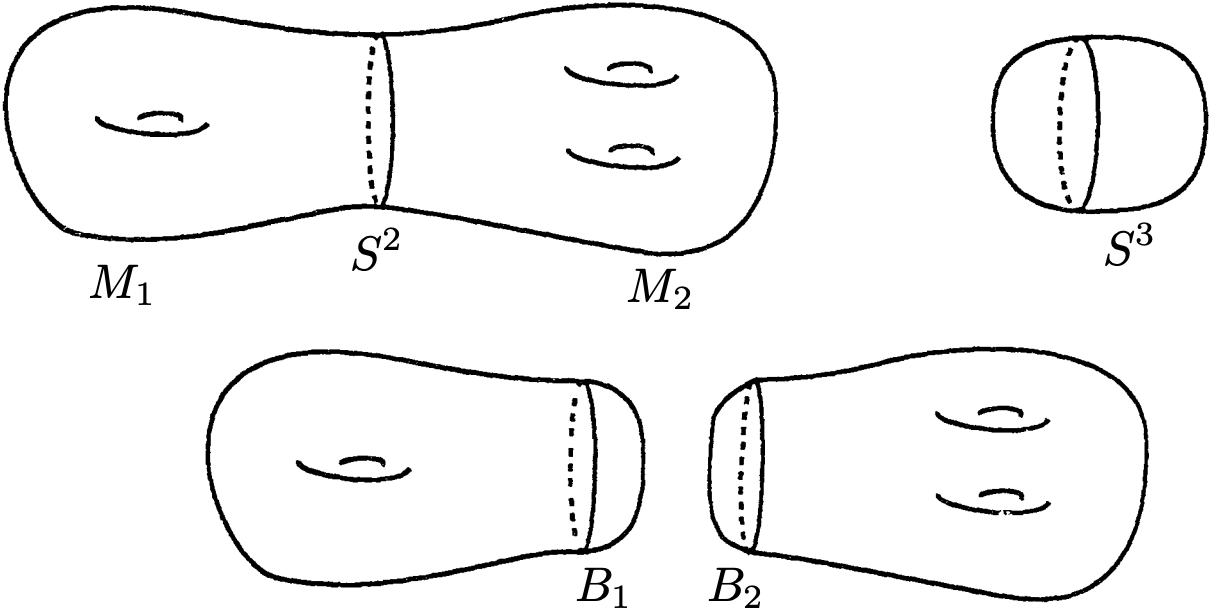
\includegraphics[width=0.85\textwidth]{figures/fig5_surgery.png}
  \caption{沿 $S^2$ 拆解 $M=M_1\#M_2$，并用 $S^3$ 的帽子把两块补圆。（原文 Figure 5，原文 p.31）}
  \label{fig:surgery}
\end{figure}

\paragraph{手术}
% 原文标题：Surgery.
前述讨论可以推广到包含威尔逊圈的情形；这会增大希尔伯特空间的维数，使线性代数更繁——人们会遇到 skein 关系等等——但总体图景基本相同。这一练习的副产品是：我们学会了如何显式计算 $S^3$ 中威尔逊圈的期望值。（这正是我们在 \S\ref{sec:3.4} 中未能兑现的一项任务。）手握 $S^3$ 上的期望值，人们就会梦想计算其他 3-流形
% ==== 原文 p.32 ====
$M\ne S^3$ 上的期望值。手术正是在这里登场：在任意 3-流形 $M$ 中给定一个纽结 $\gamma$，我们可以把 $\gamma$ 加粗成一根管 $T$，其拓扑是实心环面；从 $M$ 中挖去 $T$，对环面边界 $\partial T=T^2$ 施加一个巧妙选取的微分同胚，再把各块粘回去，就得到一个新的 3-流形 $\widetilde{M}$。三维拓扑学的一个基础结果是：任何 3-流形都可以由任何另一个经有限次沿嵌入纽结的手术得到。特别地，只要仔细考察手术对 $S^3$ 中威尔逊圈期望值做了什么，上述梦想就会实现。这正是 Witten 的做法。

% [Tutor Note: 含糊点] 「任何 3-流形可由任何另一个经有限次手术得到」= Lickorish–Wallace 定理（闭可定向 3-流形可由 S³ 沿链环作整系数 Dehn 手术得到）；原文未提 Kirby 移动与不变量良定义性。
\begin{yizhu}[含糊点]
「任何 3-流形都可以由任何另一个经有限次手术得到」是 Lickorish--Wallace 定理：任何闭可定向 3-流形都能由 $S^3$ 沿某个链环做整系数 Dehn 手术得到；原文的「从任意到任意」只是先回到 $S^3$ 再出来。要让 Witten 的论证闭合，还须说明手术描述的冗余（Kirby 移动）不改变结果，原文未提；而这一点恰是手术不变量良定义性的所在。
\end{yizhu}

事实上，这一论证与上面的论证几乎相同。从 $M=S^3$ 中挖去实心环面 $T$ 后，$T$ 与纽结补 $N=S^3\setminus T$ 的边界上各自驻留着一对典范对偶的希尔伯特空间 $\mathcal{H}_{T^2}$ 与 $\mathcal{H}_{\partial N}=\mathcal{H}^{*}_{T^2}$。$T$ 与 $N$ 上的路径积分分别给出向量 $|\psi\rangle\in\mathcal{H}_{T^2}$ 与 $|\chi\rangle\in\mathcal{H}_{\partial N}$；环面边界 $\partial T=T^2$ 上的微分同胚则在 $\mathcal{H}_{T^2}$ 上诱导一个线性变换 $K$，把 $|\psi\rangle\mapsto K|\psi\rangle$。于是新流形 $\widetilde{M}$ 上的路径积分通过算子 $K$ 与 $\mathcal{Z}(M)=\langle\chi|\psi\rangle$ 相联系：$\mathcal{Z}(\widetilde{M})=\langle\chi|K|\psi\rangle$。Witten 随后依据费林德的工作 [28] 描述亏格一的 CS 希尔伯特空间；他在 $T^2$ 上做一个模变换，靠手术从 $S^2\times S^1$ 得到 $S^3$，再借助亏格一的希尔伯特空间导出 $S^3$ 上 CS 配分函数的公式 \eqref{eq:3.32}。此后，整套程序再带源重复一遍。

% [Tutor Note: 易错点] H_{T²} 与 H_{∂N}=H*_{T²} 是同一亏格一空间的对偶写法（∂N=−T² 的定向负号已吸收进 *）；K 作用在 H_{T²} 上、夹在 ⟨χ| 与 |ψ⟩ 之间，误当作用于 H* 会给出转置。
\begin{yizhu}[易错点]
原文的记号要分清：$\mathcal{H}_{T^2}$ 是 $T$ 的边界上的希尔伯特空间，$\mathcal{H}_{\partial N}=\mathcal{H}^{*}_{T^2}$ 是纽结补的；二者本是同一个亏格一空间，星号只标对偶。$\partial T=T^2$ 与 $\partial N=-T^2$ 定向相反，这个负号已吸收进对偶里。$K$ 由 $\partial T$ 上的微分同胚诱导，作用在 $\mathcal{H}_{T^2}$ 上，故 $\langle\chi|K|\psi\rangle$ 中 $K$ 夹在对偶态与态之间；若误把 $K$ 当作作用于 $\mathcal{H}^{*}$，就得换成转置 $K^{T}$，配分函数随之改变。
\end{yizhu}

% =============================================================================
% 汇报（片段 s04b，对应原文 p.28–32）
% 覆盖：4.2 带源的量子化（p.28–29）、4.3 例：亏格零（p.29–31）、4.4 展望：手术与源（p.31–32）
% 编号公式：3 个 —— (4.5)(4.6)(4.7)，均以 \tag 锁定、顺序照原文
% 图：图 5（figures/fig5_surgery.png，width=0.85\textwidth，label=fig:surgery），位于 (4.7) 之后
% 脚注：原文脚注 9（p.29）已全译
% 译注：12 条 —— 易错点 5、含糊点 4、原文疑误 2、物理图像 1；每条前一行类型摘要注释
% 原文疑误（均照录并批注）：
%   1) p.30 毛球定理 => P^1 上无平坦联络、模空间为空：论证不成立（S^2 单连通，平凡丛平坦联络
%      模空间是单点 A=0）；结论「亏格零无标记时希尔伯特空间 1 维」不受影响。同页 nonwhere 应为 nowhere。
%   2) p.30 两标记点末句「R_2 ≠ R_1」应为「R_2 ≠ \bar R_1」。
% 存疑：无。图 4 的交叉引用用 \ref{fig:cut}（s04a 的 label），(2.27)/(3.32) 分别用 \eqref。
% 与 s01 一致：小节内的 run-in 小标题用 \paragraph{…} 且以半角句点收束；若 Lead 统一改为全角「。」请全局替换。
% =============================================================================
% >>>>>>>>>>>>>>>> end sections/s04b-hilbert2.tex <<<<<<<<<<<<<<<<

% >>>>>>>>>>>>>>>> sections/s05-wrapup.tex <<<<<<<<<<<<<<<<
% =============================================================================
%  s05-wrapup.tex —— 原文 §5 Tying Up Loose Ends（p.32–36）与 References（p.36–38）
%  编号公式：(5.1)–(5.4)
% =============================================================================

% ==== 原文 p.32 ====
\section{收束：未竟之结}\label{sec:5}
% 原文标题：Tying Up Loose Ends

% [Tutor Note: 本节重点] 物理图像 / 数学工具 / 主要结论
\begin{keytakeaways}
\begin{itemize}[leftmargin=1.4em,itemsep=2pt,topsep=2pt]
  \item \textbf{物理图像：}三维体里的陈--西蒙斯理论与它边界上的二维共形场论是同一套数据的两种说法：体中的威尔逊线在边界上化成原初场的算符插入，这正是全息对偶的原型。把规范群换成非紧的庞加莱群，三维引力本身也变成一个陈--西蒙斯理论。
  \item \textbf{数学工具：}琼斯多项式及其 skein 关系与变量 $q$、连通和下配分函数的乘法性质 \eqref{eq:4.7}、Segal 的模函子 \cite{segal} 与共形块、韦斯--朱米诺--维滕模型的作用量、二次卡西米尔 $c_2(G)$。
  \item \textbf{主要结论：}$G=\mathrm{SU}(N)$ 时正确变量是 $q=\exp[2\pi i/(k+N)]$（只有树图级才是 $e^{2\pi i/k}$）；无结的威尔逊圈期望值为 $(q^{N/2}-q^{-N/2})/(q^{1/2}-q^{-1/2})$；一圈修正等价于 $k\to k+c_2(G)/2$，对应二维 CFT 的中心荷 $c=kd/(k+N)$。
\end{itemize}
\end{keytakeaways}

\paragraph{统一的视角}
% 原文标题：A unified view.
在这篇综述里，我们试着理清陈--西蒙斯理论背后潜伏的那些拓扑与几何。旅程从 \S\ref{sec:2} 开始：我们先请出 $\mathrm{U}(1))$ 理论，视角或许取自一位初次撞见其怪异物理的实验物理学家。这段穿越阿贝尔理论的现象学漫游，为随后用路径积分（\S\ref{sec:3}）和正则量子化（\S\ref{sec:4}）对非阿贝尔理论作更形式化的处理做了铺垫。一路上，我们刻意不谈 CS 理论所处的那个更大的物理与数学世界中的许多侧面。下面我们先对已经走过的这条窄路作最后一次回顾，再匆匆一瞥那个更大世界的若干角落，以此作结。

\subsection{全景回顾}\label{sec:5.1}
% 原文标题：Broad Recapitulation

\paragraph{阿贝尔理论}
在 \S\ref{sec:2} 中我们发现，CS 理论是拓扑的。它最简单的物理可观测对象是任意子交换相位，这些相位度量的是附着在平面上游走电荷上的磁通线绕了多少圈。我们很快认出，这些相位就是威尔逊圈的期望值，而用路径积分处理威尔逊圈最为自然。纯 CS 路径积分告诉我们：有磁通存在时，为保住量子理论的规范不变性，陈--西蒙斯能级 $k$ 必须量子化成整数。
% ==== 原文 p.33 ====
带源的 CS 路径积分则表明，任意子相位真正抓住的是拓扑不变量——源所附威尔逊圈扫出的那些纽结的环绕数。此后我们用正则形式处理 $\mathrm{U}(1))$ 理论，发现哈密顿量恒为零，CS 规范场的各个分量彼此正则共轭。我们在 $\R^2$ 上精确解出了这个理论，只得到一个物理态；讨论了它在 $T^2$ 上有限维的可观测代数；最后以若干有趣而重要的拓扑评述收尾。

\paragraph{路径积分}
搭起非阿贝尔规范理论的机器之后，我们引入并量子化了非阿贝尔 CS 理论，入手处是考察规范不变性在绕数非零的规范变换下如何失效。接着我们尝试在弱耦合下计算纯 CS 路径积分。这一计算给出底流形 $M$ 的一大批拓扑不变量，可结果看上去仍依赖它的度规。我们设法消掉了这份依赖，代价是加一个依赖 $M$ 标架的抵消项。最终我们得到纯 CS 理论配分函数的一个显式拓扑公式，还有一条描述它在标架变换下如何变化的规律。带威尔逊圈的路径积分有着相似的拓扑命运：为消去与威尔逊圈自环绕数相伴的发散，我们必须给纽结选定一个标架。与无源理论的类比十分紧密，我们得到一个公式，描述威尔逊圈期望值在标架变换下的变换。

\paragraph{正则量子化}
要对非阿贝尔 CS 理论作正则分析，我们把一般的三维流形 $M$ 切成若干局部形如 $\Sigma\times\R$ 的块，其中 $\Sigma$ 是黎曼面。CS 理论在 $\Sigma$ 上的经典相空间是 $\Sigma$ 上平坦联络的模空间；为量子化它，我们发展出凯勒量子化这一有力技术。这一技术把纯 CS 希尔伯特空间描述成 $M$ 上某个线丛的全纯截面空间。我们还考虑了威尔逊圈的插入：这些圈穿透 $\Sigma$，在其表面留下非阿贝尔电荷，位置是特殊点（distinguished points），也叫标记点，与阿贝尔理论里的磁通线遥相呼应。这些圈起初似乎带来无法解决的问题，连理论的经典描述也躲不开。不过，借助博雷尔--韦伊--博特定理，再靠「带对称性的系统如何量子化」这一哲学，我们微调模空间，把非阿贝尔电荷的效应算了进来。在 $\Sigma$ 亏格为零这一具体情形，能拿到的结果要具体得多，包括希尔伯特空间的完整描述及其维数。

\subsection{延伸与联系}\label{sec:5.2}
% 原文标题：Extensions and Connections

\paragraph{琼斯多项式}
Witten 那篇奠基性论文 \cite{witten1989} 的主要贡献之一，是把一个重要的纽结不变量——琼斯多项式——用 CS 理论里的威尔逊圈来解释。为陈述他的部分结果，我们先看一个在全文里无处不在的量：$e^{2\pi i/k}$。我们给它取名 $q$，并断言：从纽结理论的角度看，这正是写下最终结果所该用的变量。
% ==== 原文 p.34 ====
对复的 $k$，变量 $q=e^{2\pi i/k}$ 与椭圆函数论中出现的 nome $q=e^{2\pi i\tau}$ 关系密切。

椭圆函数与琼斯多项式 $V_q$ 都在 $k=1/\tau$（即 CS 耦合的倒数）取整数值时表现出特殊性质，这绝非巧合：量子 CS 理论的结果恰在此时变得可用。其实，这话只在所谓「树图级」上才成立：对 $G=\mathrm{SU}(N)$，正确的变量其实是 $q=\exp\left(\frac{2\pi i}{k+N}\right)$。用 nome 表示，我们终于能写下非阿贝尔 CS 理论中若干威尔逊圈的期望值。例如 $S^3$ 中一个无结的威尔逊圈 $W[\bigcirc]$，取 $\mathrm{SU}(N)$ 的基础表示，其真空期望值为
\begin{equation}\tag{5.1}\label{eq:5.1}
  \langle W[\bigcirc]\rangle
  = \frac{q^{N/2}-q^{-N/2}}{q^{1/2}-q^{-1/2}}
  \overset{N=2}{\sim} q^{1/2}+q^{-1/2}
  = \frac{\sin[2\pi/(k+2)]}{\sin[\pi/(k+2)]} .
\end{equation}

% [Tutor Note: 易错点] (5.1) 的幂次：分子为 $q^{N/2}-q^{-N/2}$、分母为 $q^{1/2}-q^{-1/2}$，且 $q$ 必须取 $q=\exp[2\pi i/(k+N)]$；若用树图的 $q=e^{2\pi i/k}$，则 $q^{1/2}+q^{-1/2}=2\cos(\pi/k)$ 与右端的 $2\cos[\pi/(k+2)]$ 不等。
\begin{yizhu}[易错点]
\eqref{eq:5.1} 的幂次要逐个核对：分子是 $q^{N/2}-q^{-N/2}$，分母是 $q^{1/2}-q^{-1/2}$，指数上的 $1/2$ 一个都不能漏。更要紧的是 $q$ 的取法：右边化成 $\sin$ 比值时用的是 $q=\exp[2\pi i/(k+N)]$；在 $N=2$ 这一支上，$q^{1/2}+q^{-1/2}=2\cos[\pi/(k+N)]$，恰等于 $\sin[2\pi/(k+N)]/\sin[\pi/(k+N)]$。若照前文的树图定义 $q=e^{2\pi i/k}$ 代入，得到 $2\cos(\pi/k)$，与 $\sin[2\pi/(k+2)]/\sin[\pi/(k+2)]=2\cos[\pi/(k+2)]$ 不等。作者在紧邻 (5.1) 之前的那句话里承认这「只在树图级上」才对，正指此处。
\end{yizhu}

% [Tutor Note: 物理图像] (5.1) 的比值是量子群 $U_q(\mathfrak{sl}_N)$ 中基础表示的量子维数 $[N]_q$，$k\to\infty$ 时回到经典维数 $N$。
\begin{yizhu}[物理图像]
\eqref{eq:5.1} 的比值不是拼凑出来的：它就是量子群 $U_q(\mathfrak{sl}_N)$ 中基础表示的量子维数 $[N]_q$，也就是无结威尔逊圈在 CS 理论里能取到的「大小」。$k\to\infty$（即 $q\to1$）时 $[N]_q\to N$，与经典维数吻合；$k$ 有限时它才明显偏离 $N$，有限能级的量子效应第一次以纯数值的形式露了面。
\end{yizhu}

代入著名的 skein 关系（Witten 也用希尔伯特空间方法导出了它），这个表达式给出无结的正确的（平凡的！）琼斯多项式：
\begin{equation}\tag{5.2}\label{eq:5.2}
  -q\,V_q(\bigcirc) + \left(q^{1/2}-q^{-1/2}\right)\langle W\rangle + q^{-1}V_q(\bigcirc) = 0
  \quad\Longrightarrow\quad V_q(\bigcirc) = 1 .
\end{equation}

% [Tutor Note: 易错点] (5.2) 三个圈同形，原文未标 $L_\pm$ 与 smoothing：标准形为 $q^{-1}V(L_+)-qV(L_-)=(q^{1/2}-q^{-1/2})V(L_0)$，故首项应读作 $L_-$、末项读作 $L_+$、中间项读作 smoothing；且 (5.2) 的整体符号与标准形相反。
\begin{yizhu}[易错点]
\eqref{eq:5.2} 里三个圈都写作 $\bigcirc$，原文没有标注哪两个是 $L_\pm$、哪一个是 smoothing。标准的 Jones skein 关系是 $q^{-1}V(L_+)-qV(L_-)=(q^{1/2}-q^{-1/2})V(L_0)$；据此，首项 $-qV_q(\bigcirc)$ 应读作 $L_-$，末项 $q^{-1}V_q(\bigcirc)$ 应读作 $L_+$，中间的 $\langle W\rangle$ 才是 smoothing 后得到的链环。还要留意符号：标准归一化下二分量平凡链环的 $V(L_0)=-(q^{1/2}+q^{-1/2})$，而 \eqref{eq:5.1} 在 $N=2$ 时取正号，所以 \eqref{eq:5.2} 隐含的符号约定与标准形差一个整体符号。核对时以「把 \eqref{eq:5.1} 代进去后化为恒等式」为准，不要逐项对号。
\end{yizhu}

事实上，琼斯多项式的若干初等性质，从 \S\ref{sec:4.4} 的讨论里已经能看出来。比如，因子化结果 \eqref{eq:4.7} 可以写成
\begin{equation}\tag{5.3}\label{eq:5.3}
  \frac{\mathcal{Z}(M)}{\mathcal{Z}(S^3)}
  = \frac{\mathcal{Z}(M_1)}{\mathcal{Z}(S^3)}\cdot\frac{\mathcal{Z}(M_2)}{\mathcal{Z}(S^3)} .
\end{equation}
把威尔逊圈也算进来时，上面出现的那些比率就变成琼斯多项式；公式于是表达了它们在连通和下的乘性行为。

% [Tutor Note: 易错点] (5.3) 的乘性只对分处连通和两片的链环成立；比率用 $\mathcal{Z}(S^3)$ 归一化正是为了与 $V_q(\text{无结})=1$ 对齐，而同在 $S^3$ 里不相交的两个平凡圈各给出因子 $-(q^{1/2}+q^{-1/2})$，不是 $1$。
\begin{yizhu}[易错点]
\eqref{eq:5.3} 的乘性不可越界使用：它说的是连通和 $M_1\#M_2$ 的配分函数等于两片各自配分函数之积再除以一个 $\mathcal{Z}(S^3)$，对应的链环分处两片。若把两个圈放进同一个 $S^3$，Jones 多项式要对每个分裂出的平凡分量各乘一个因子 $-(q^{1/2}+q^{-1/2})$，结果不是 $1$。比率用 $\mathcal{Z}(S^3)$ 归一化，恰好让空流形对应 $1$、无结对应 $V_q(\bigcirc)=1$；把这两件事混为一谈，是本节最容易犯的错。
\end{yizhu}

\paragraph{与二维 CFT 的关系}
% 原文标题：Relation to 2D CFT.
到此为止，我们一直刻意不谈 CS 理论与二维共形场论之间的深刻联系。完整处理这些联系超出本综述的范围，但不妨在此收集几条提示性的评论。第一条线索来自 \S\ref{sec:3.2} 中我们对纯 CS 理论配分函数的路径积分计算。领头阶结果 \eqref{eq:3.10} 与一圈结果 \eqref{eq:3.27} 的主要差别，除复杂度增加之外，就是组成配分函数的那些相对相位整体平移了，仿佛我们已经把 $k$ 换成 $k+\frac{c_2(G)}{2}$：
\begin{equation}\tag{5.4}\label{eq:5.4}
  \exp\left(ik\,I[A^{(\alpha)}]\right)
  \;\leadsto\;
  \exp\left[i\left(k+\frac{c_2(G)}{2}\right)I[A^{(\alpha)}]\right] .
\end{equation}

% [Tutor Note: 易错点] (5.4) 的 $k\to k+c_2(G)/2$ 与紧随其后的 $c=kd/(k+N)$ 靠 $c_2(G)$ 的归一化配平：作者用 $c_2(\mathrm{SU}(2))=4$，故 $c_2(G)/2=h^\vee$，$\mathrm{SU}(N)$ 时即 $N$；换用 $\Tr_{\rm fund}(T^aT^b)=\frac12\delta^{ab}$ 的归一化则平移应写成 $k+c_2(G)$。
\begin{yizhu}[易错点]
\eqref{eq:5.4} 的平移 $k\to k+c_2(G)/2$ 与紧随其后的中心荷公式 $c=\frac{kd}{k+N}$ 看似差一个因子，其实靠 $c_2(G)$ 的归一化配平：作者在 \eqref{eq:3.32} 之后注明 $c_2(\mathrm{SU}(2))=4$，可见他把 $c_2(G)$ 归一化成 $2h^\vee$（$h^\vee$ 为对偶考克斯特数），于是 $c_2(G)/2=h^\vee$，$\mathrm{SU}(N)$ 时恰为 $N$。这正好是 $q=\exp[2\pi i/(k+N)]$ 与 $c=\frac{kd}{k+N}$ 里的那个 $N$。若改用物理文献常见的 $\Tr_{\rm fund}(T^aT^b)=\frac12\delta^{ab}$ 归一化，$c_2(\mathrm{SU}(2))=2$，平移要写成 $k+c_2(G)$；照字面读成 $k+1$ 会差一倍。
\end{yizhu}

这让人想起二维 CFT 中的类似现象：只要把近似公式里的参数平移，许多半经典结果就变成精确的。实际上，当 $G=\mathrm{SU}(N)$ 时，$k$ 与某个二维 CFT 的中心荷 $c$ 由公式 $c=\frac{kd}{k+N}$ 相联系，其中 $d=\dim G=N^2-1$。CS 耦合弱时 $k\to\infty$，于是 $c\to d$。这样一来（从 CFT 的观点看）毫不奇怪：
% ==== 原文 p.35 ====
CS 理论里在大 $k$ 下导出的许多结果，例如配分函数的标架变换规律 \eqref{eq:3.28}，都有把 $d$ 换成 $c$ 得到的推广。威尔逊圈的标架变换规律 \eqref{eq:3.31} 上演着相似的故事；这一回，因子 $\frac{n_a^2}{2k}$ 换成了某个 CFT 原初场的共形权重 $h$。更一般地，CS 理论中标架化这一概念，在相应 CFT 的单值性里有直接的对应物。

\paragraph{全息对偶}
% 原文标题：Holographic duality.
读到这里应该清楚：三维的 CS 理论与二维的共形场论关系密切。我们握有大量证据：其一，上面那些类比本身就足够撩人。其二，在 \S\ref{sec:4} 中我们瞥见：CS 理论的希尔伯特空间与配分函数，来自沿黎曼面切分三维流形，并仔细照料这些低维边界上的物理。我们在那里遇到的构造——黎曼面的模空间、平坦联络的模空间、全纯向量丛、单值性、表示的融合——都是二维 CFT 的重要配料。其中或许最重要的，是 Segal 的模函子 \cite{segal}。在 Segal 的原始表述里，一张黎曼面 $\Sigma$ 定义了二维 CFT 所栖身的时空；与这个时空对应的是一个向量空间 $\mathcal{H}_\Sigma$，由单位算符的后代所满足的共形沃德恒等式的解组成。Segal 对这个「共形块空间」的构造，与我们对 $\Sigma\times\R$ 上 CS 希尔伯特空间的构造完全同一；这就把 CS 与 CFT 两种理论的等价牢牢确立下来。确实可以验证：我们算出的带源 CS 希尔伯特空间的维数，与对应带标记点黎曼面上二维 CFT 的共形块数目一致。

% [Tutor Note: 含糊点] 「完全同一」「牢牢确立」跳过了要验证的东西：Segal 模函子 [24] 与 CS 几何量子化给出同一组共形块，须核对维数（Verlinde [28]、Moore--Seiberg [29,30]）、拼接相容性与单值性相位三件事。
\begin{yizhu}[含糊点]
「完全同一」与「牢牢确立」两句跨过了实质验证。模函子（Segal \cite{segal}）是从带标记黎曼面到向量空间的函子，配以拼接相容性：它把 $\Sigma$ 映成共形块空间，把拼接映成线性映射的复合。CS 一侧给出的则是平坦联络模空间上的全纯截面（几何量子化）。要说两者等同，至少要核对三件事：维数公式一致（融合规则与 Verlinde 公式 \cite{verlinde1988}，Moore--Seiberg \cite{moore1989,moore1988} 的讨论）、拼接映射与 CS 粘合相容、标架与单值性的相位一致。原文只点出了亏格零情形的维数吻合。另可留意：它把 $\mathcal{H}_\Sigma$ 说成「单位算符的后代」的解空间，这其实是真空（无插入）情形的说法；带标记点时须换成相应原初场的后代，紧接着的维数断言才有着落。
\end{yizhu}

现在轮廓渐渐显出的图景是一张全息图：三维流形 $M$ 上的 CS 理论，等价于（或说对偶于）栖身在黎曼面 $\Sigma$ 上的某个二维 CFT，而 $\Sigma$ 可以看作 $M$ 的「边界」。（在我们关于拼接与手术的讨论里，这个解释是我们硬按上去的。）相应的 CFT 叫韦斯--朱米诺--维滕（WZW）模型，它的作用量与 CS 作用量变分中那个边界项 \eqref{eq:3.4} 颇为相像。在这个框架里，CS 威尔逊线穿透 $\Sigma$ 处的标记点，代表 WZW 模型里原初场的算符插入，这些原初场按威尔逊线所附的表示变换。CS--WZW 对应是一条真正的定理，可以看作全息原理的原型。

% [Tutor Note: 含糊点] 「颇为相像」可落到实处：(3.4) 的第二项 $\frac{k}{4\pi}\int\frac13\Tr[(g^{-1}\partial g)^3]$ 正是 WZW 作用量的 Wess--Zumino 项，即纯规范 $A=g^{-1}\dd g$ 的 CS 作用量在 3 维球上的取值。
\begin{yizhu}[含糊点]
「颇为相像」不是修辞，落到实处是这样：\eqref{eq:3.4} 的第二项 $\frac{k}{4\pi}\int_M\frac{1}{3}\Tr[(g^{-1}\partial g)^3]$ 正是 WZW 作用量的 Wess--Zumino 项。把二维边界 $\Sigma$ 换成以它为边界的 3 维球 $B$，并把 $g$ 延拓进 $B$，该项就是 $\frac{k}{12\pi}\int_B\Tr(g^{-1}\dd g)^3$，即纯规范 $A=g^{-1}\dd g$ 的 CS 作用量。换言之，WZW 作用量 = $\Sigma$ 上的动能项 + CS 作用量在纯规范上的取值；CS--WZW 对应在作用量层面就体现在这里。\eqref{eq:3.4} 的第一项是全导数，搬到边界上化为 $\Sigma$ 的边界积分。
\end{yizhu}

\paragraph{三维引力}
% 原文标题：3D gravity.
有一个重要因素使 CS--WZW 算不上全息对偶的真实例子：对应关系的 CS 一侧没有引力物理。然而 Witten 表明 \cite{witten1988}，三维引力就是一个陈--西蒙斯理论！广义相对论的爱因斯坦场方程在 $2+1$ 维不允许引力波解。因此这个理论没有局部传播自由度；正因如此，它是纯拓扑的。支配该理论的爱因斯坦--希尔伯特作用量有标架场与自旋联络的一阶表述，Witten 表明它可以改写成形如 \eqref{eq:3.3} 的 CS 作用量。三维引力里的「规范场」取值于庞加莱群 $\mathrm{ISO}(2,1)$ 的李代数，或它的某个非紧变体；
% ==== 原文 p.36 ====
具体取哪个，取决于宇宙学常数的符号。（对德西特背景，群是 $\mathrm{SO}(3,1)$；对反德西特，是 $\mathrm{SO}(2,2)$。）由于规范群不再紧致，紧致李群理论的许多内容不再适用，理论也就更难解释。尽管有这份困难，Witten 仍论证 \cite{witten2007}，三维引力容许一个良定义的量子化，与我们在本文所见 CS 理论的量子化类似。这一结论把 CS--WZW 对应确立为 $\mathrm{AdS}_3/\mathrm{CFT}_2$ 对偶的一个真实化身。Witten 还论证该理论无论经典还是量子都精确可解。即便如此，关于这个对偶及其对量子引力的含义，仍有太多东西有待理解。

% [Tutor Note: 含糊点] 「无引力波 \$\\ 无局部自由度 \$\\ 纯拓扑」跳过了一步：2+1 维度规 6 个分量减 3 个微分同胚、3 个约束得 0 个局部自由度；拓扑性来自 Witten [31] 的一阶表述，标架场与自旋联络并成 ISO(2,1)（或 SO(3,1)/SO(2,2)）值联络，作用量即 CS 形式且不含度规。
\begin{yizhu}[含糊点]
「没有引力波 \$\\ 没有局部传播自由度 \$\\ 纯拓扑」跳过了中间一步。2+1 维度规有 6 个分量，减去 3 个微分同胚自由度与 3 个（1 个哈密顿 + 2 个动量）约束，局部自由度恰好为 0；这才是计数上的理由。拓扑性的来源则是 Witten \cite{witten1988} 的一阶表述：标架场 $e^a$ 与自旋联络 $\omega^a$ 并成 $\mathrm{ISO}(2,1)$（或 $\mathrm{SO}(3,1)$、$\mathrm{SO}(2,2)$）值联络 $\mathcal{A}=e^aP_a+\omega^aJ_a$，爱因斯坦--希尔伯特作用量 $\int e\wedge(d\omega+\omega\wedge\omega)$ 就是 \eqref{eq:3.3} 形状的 CS 作用量；作用量里不含度规，故不依赖度规。非紧群使 \cite{witten1989} 那套紧致李群论证失效，这正是 \cite{witten2007} 要处理的技术难点。
\end{yizhu}

% ==== 原文 p.36 下半页：References ====
\begin{thebibliography}{32}

\bibitem{witten1989} E. Witten, ``Quantum Field Theory and the Jones Polynomial,'' \emph{Commun. Math. Phys.} \textbf{121}, 351--399 (1989) doi:10.1007/BF01217730

\bibitem{dunne} G. V. Dunne, ``Aspects of Chern-Simons theory,'' [arXiv:hep-th/9902115 [hep-th]]

\bibitem{tong_gauge} D. Tong, ``Gauge Theory,'' ch. 8, damtp.cam.ac.uk/user/tong/gaugetheory/gt.pdf

\bibitem{tong_qhe} D. Tong, ``Lectures on the Quantum Hall Effect,'' ch. 5, [arXiv:1606.06687 [hep-th]]

\bibitem{chern1974} S.-S. Chern and J. Simons, ``Characteristic forms and geometric invariants,'' \emph{Ann. Math.} \textbf{99} (1), 48--69 (1974) doi:10.2307/1971013

\bibitem{polyakov1988} A. M. Polyakov, ``Fermi--Bose Transmutations Induced by Gauge Fields,'' \emph{Mod. Phys. Lett. A} \textbf{3}, 325 (1988) doi:10.1142/S0217732388000398

\bibitem{ricca2011} R. L. Ricca and B. Nipoti, ``Gauss' Linking Number Revisited,'' \emph{J. Knot Theory Ramif.}, \textbf{20} (10), 1325--1343 (2011) doi:10.1142/S0218216511009261

\bibitem{achucarro1986} A. Achucarro and P. K. Townsend, ``A Chern-Simons Action for Three-Dimensional anti-De Sitter Supergravity Theories,'' \emph{Phys. Lett. B} \textbf{180}, 89 (1986) doi:10.1016/0370-2693(86)90140-1

\bibitem{steenrod1951} N. Steenrod. \emph{The Topology of Fibre Bundles (PMS-14)}, Princeton University Press (1951) JSTOR, \href{https://www.jstor.org/stable/j.ctt1bpm9t5}{www.jstor.org/stable/j.ctt1bpm9t5}

\bibitem{nakahara} M. Nakahara, ``Geometry, Topology and Physics,'' ch. 9--10

\bibitem{coleman} S. Coleman, ``Aspects of Symmetry: Selected Erice Lectures,'' \S7.3.2 doi:10.1017/CBO9780511565045

\bibitem{bott1956} R. Bott, ``An Application of the Morse Theory to the Topology of Lie Groups,'' \emph{Bulletin de la S.M.F.} \textbf{84}, 251--281 (1956), doi:10.24033/bsmf.1472, \href{http://www.numdam.org/articles/10.24033/bsmf.1472}{http://www.numdam.org/articles/10.24033/bsmf.1472}

% ==== 原文 p.37 ====
\bibitem{barnatan1991} D. Bar-Natan and E. Witten, ``Perturbative expansion of Chern-Simons theory with noncompact gauge group,'' \emph{Commun. Math. Phys.} \textbf{141}, 423--440 (1991) doi:10.1007/BF02101513

\bibitem{schwarz1978} A. S. Schwarz, ``The Partition Function of Degenerate Quadratic Functional and Ray-Singer Invariants,'' \emph{Lett. Math. Phys.} \textbf{2}, 247--252 (1978) doi:10.1007/BF00406412

\bibitem{aps1975} M. F. Atiyah, V. K. Patodi, and I. M. Singer, ``Spectral asymmetry and Riemannian Geometry 1,'' \emph{Math. Proc. Cambridge Phil. Soc.} \textbf{77}, 43 (1975) doi:10.1017/S0305004100049410

\bibitem{aps1976a} M. F. Atiyah, V. K. Patodi, and I. M. Singer, ``Spectral asymmetry and Riemannian geometry 2,'' \emph{Math. Proc. Cambridge Phil. Soc.} \textbf{78}, 405 (1976) doi:10.1017/S0305004100051872

\bibitem{aps1976b} M. F. Atiyah, V. K. Patodi, and I. M. Singer, ``Spectral asymmetry and Riemannian geometry 3,'' \emph{Math. Proc. Cambridge Phil. Soc.} \textbf{79}, 71--99 (1976) doi:10.1017/S0305004100052105

\bibitem{parker1984} P. E. Parker, ``On Some Theorems of Geroch and Stiefel,'' \emph{J. Math. Phys.} \textbf{25}, 597 (1984) doi:10.1063/1.526209

\bibitem{milnor1974} J. W. Milnor and J. D. Stasheff, \emph{Characteristic Classes} (AM-76) (1974) doi:10.1515/9781400881826

\bibitem{elhamdadi2020} M. Elhamdadi, M. Hajij, and K. Istvan, ``Framed Knots,'' \emph{Math. Intell.} \textbf{42}, 7--22 (2020) \href{https://link.springer.com/content/pdf/10.1007/s00283-020-09990-0.pdf}{https://link.springer.com/content/pdf/10.1007/s00283-020-09990-0.pdf}

\bibitem{atiyahbott1982} M. F. Atiyah and R. Bott, ``The Yang-Mills equations over Riemann surfaces,'' \emph{Phil. Trans. Roy. Soc. Lond. A} \textbf{308}, 523--615 (1982)

\bibitem{woodhouse} N. Woodhouse, ``Geometric Quantization.''

\bibitem{quillen1986} D. Quillen, ``Determinants of Cauchy--Riemann operators over a Riemann surface,'' \emph{Fuct. Anal. Appl.} \textbf{19}, 31 (1986)

\bibitem{segal} G. Segal, ``Conformal field theory,'' Oxford preprint; and lecture at the IAMP Congress, Swansea, July, 1988

\bibitem{connes2006} A. Connes and M. Marcolli, ``A Walk in the noncommutative garden,'' [arXiv:math/0601054 [math.QA]].

\bibitem{kirillov2004} A. A. Kirillov, \emph{Lectures on the Orbit Method}, American Mathematical Soc., \textbf{64} (2004) doi:10.1090/gsm/064

% ==== 原文 p.38 ====
\bibitem{beasley2013} C. Beasley, ``Localization for Wilson Loops in Chern-Simons Theory,'' \emph{Adv. Theor. Math. Phys.} \textbf{17}, no.1, 1-240 (2013) doi:10.4310/ATMP.2013.v17.n1.a1 [arXiv:0911.2687 [hep-th]].

\bibitem{verlinde1988} E. P. Verlinde, ``Fusion Rules and Modular Transformations in 2D Conformal Field Theory,'' \emph{Nucl. Phys. B} \textbf{300}, 360-376 (1988) doi:10.1016/0550-3213(88)90603-7

\bibitem{moore1989} G. W. Moore and N. Seiberg, ``Classical and Quantum Conformal Field Theory,'' \emph{Commun. Math. Phys.} \textbf{123}, 177 (1989) doi:10.1007/BF01238857

\bibitem{moore1988} G. W. Moore and N. Seiberg, ``Polynomial Equations for Rational Conformal Field Theories,'' \emph{Phys. Lett. B} \textbf{212}, 451-460 (1988) doi:10.1016/0370-2693(88)91796-0

\bibitem{witten1988} E. Witten, ``(2+1)-Dimensional Gravity as an Exactly Soluble System,'' \emph{Nucl. Phys. B} \textbf{311}, 46 (1988) doi:10.1016/0550-3213(88)90143-5

\bibitem{witten2007} E. Witten, ``Three-Dimensional Gravity Revisited,'' [arXiv:0706.3359 [hep-th]].

\end{thebibliography}

% =============================================================================
% 汇报（s05-wrapup.tex）
% * 覆盖：原文 p.32「A unified view.」至 p.36 §5 末；参考文献 [1]--[32]（p.36--38）
% * 页锚点：p.32--p.38 共 7 个，p.33/p.34/p.36 三处原文断页在句中，锚点就近放在分句处
% * 编号公式：4 个，(5.1)--(5.4)，\tag 逐字照原文；(5.4) 的波浪箭头按 amssymb 用 \leadsto
%   （lint.py 的 \left/\right 计数会把 \rightsquigarrow 误计为 \right，故未用后者）
% * 译注：8 条（易错点 4、含糊点 3、物理图像 1）
% * 文献：32 条，键名与顺序照 SPEC §8；卷号/页码/doi/arXiv 号逐条对 p.36--38 图像核过，
%   未见缺漏或数字错字。原文自身笔误照录并在下方登记。
% * 原文笔误：[23] 期刊缩写作「Fuct. Anal. Appl.」（应为 Funct.）；[22] 作者名作
%   「N. Woodhouse」（通行作 N. M. J. Woodhouse）；[9] 作者名后为句点而非逗号。
% * 记号：群名按原文排成直立体 \mathrm{SU}/\mathrm{ISO}/\mathrm{SO}，与 s04a/s04b 一致
%   （s01 用斜体，Lead 可统一）；(5.3) 的配分函数按 p.34 图像用 \mathcal{Z}，与 s04b 一致。
% * 存疑：q=e^{2πi/k}（树图）与 q=exp(2πi/(k+N))（正确）作者先给后改，已照原文层次
%   译出；c=kd/(k+N) 中的 k 已是重整化能级，与树图 k 同符号，已在译注点明。
% =============================================================================
% >>>>>>>>>>>>>>>> end sections/s05-wrapup.tex <<<<<<<<<<<<<<<<


\end{document}
